%%
% Copyright (c) 2017 - 2020, Pascal Wagler;
% Copyright (c) 2014 - 2020, John MacFarlane
%
% All rights reserved.
%
% Redistribution and use in source and binary forms, with or without
% modification, are permitted provided that the following conditions
% are met:
%
% - Redistributions of source code must retain the above copyright
% notice, this list of conditions and the following disclaimer.
%
% - Redistributions in binary form must reproduce the above copyright
% notice, this list of conditions and the following disclaimer in the
% documentation and/or other materials provided with the distribution.
%
% - Neither the name of John MacFarlane nor the names of other
% contributors may be used to endorse or promote products derived
% from this software without specific prior written permission.
%
% THIS SOFTWARE IS PROVIDED BY THE COPYRIGHT HOLDERS AND CONTRIBUTORS
% "AS IS" AND ANY EXPRESS OR IMPLIED WARRANTIES, INCLUDING, BUT NOT
% LIMITED TO, THE IMPLIED WARRANTIES OF MERCHANTABILITY AND FITNESS
% FOR A PARTICULAR PURPOSE ARE DISCLAIMED. IN NO EVENT SHALL THE
% COPYRIGHT OWNER OR CONTRIBUTORS BE LIABLE FOR ANY DIRECT, INDIRECT,
% INCIDENTAL, SPECIAL, EXEMPLARY, OR CONSEQUENTIAL DAMAGES (INCLUDING,
% BUT NOT LIMITED TO, PROCUREMENT OF SUBSTITUTE GOODS OR SERVICES;
% LOSS OF USE, DATA, OR PROFITS; OR BUSINESS INTERRUPTION) HOWEVER
% CAUSED AND ON ANY THEORY OF LIABILITY, WHETHER IN CONTRACT, STRICT
% LIABILITY, OR TORT (INCLUDING NEGLIGENCE OR OTHERWISE) ARISING IN
% ANY WAY OUT OF THE USE OF THIS SOFTWARE, EVEN IF ADVISED OF THE
% POSSIBILITY OF SUCH DAMAGE.
%%

%%
% This is the Eisvogel pandoc LaTeX template.
%
% For usage information and examples visit the official GitHub page:
% https://github.com/Wandmalfarbe/pandoc-latex-template
%%

% Options for packages loaded elsewhere
\PassOptionsToPackage{unicode}{hyperref}
\PassOptionsToPackage{hyphens}{url}
\PassOptionsToPackage{dvipsnames,svgnames*,x11names*,table}{xcolor}
%
\documentclass[
  paper=a4,
  oneside  ,captions=tableheading
]{scrbook}
\usepackage{lmodern}
\usepackage{setspace}
\setstretch{1.2}
\usepackage{amsmath}
\usepackage{ifxetex,ifluatex}
\ifnum 0\ifxetex 1\fi\ifluatex 1\fi=0 % if pdftex
  \usepackage[T1]{fontenc}
  \usepackage[utf8]{inputenc}
  \usepackage{textcomp} % provide euro and other symbols
  \usepackage{amssymb}
\else % if luatex or xetex
  \usepackage{unicode-math}
  \defaultfontfeatures{Scale=MatchLowercase}
  \defaultfontfeatures[\rmfamily]{Ligatures=TeX,Scale=1}
\fi
% Use upquote if available, for straight quotes in verbatim environments
\IfFileExists{upquote.sty}{\usepackage{upquote}}{}
\IfFileExists{microtype.sty}{% use microtype if available
  \usepackage[]{microtype}
  \UseMicrotypeSet[protrusion]{basicmath} % disable protrusion for tt fonts
}{}
\makeatletter
\@ifundefined{KOMAClassName}{% if non-KOMA class
  \IfFileExists{parskip.sty}{%
    \usepackage{parskip}
  }{% else
    \setlength{\parindent}{0pt}
    \setlength{\parskip}{6pt plus 2pt minus 1pt}}
}{% if KOMA class
  \KOMAoptions{parskip=half}}
\makeatother
\usepackage{xcolor}
\definecolor{default-linkcolor}{HTML}{A50000}
\definecolor{default-filecolor}{HTML}{A50000}
\definecolor{default-citecolor}{HTML}{4077C0}
\definecolor{default-urlcolor}{HTML}{4077C0}
\IfFileExists{xurl.sty}{\usepackage{xurl}}{} % add URL line breaks if available
\IfFileExists{bookmark.sty}{\usepackage{bookmark}}{\usepackage{hyperref}}
\hypersetup{
  pdftitle={Appunti Programmazione 1 - Riccardi},
  pdfauthor={Giovanni Foletto; Enrico Carnelos; Stefano Viel},
  hidelinks,
  breaklinks=true,
  pdfcreator={LaTeX via pandoc with the Eisvogel template}}
\urlstyle{same} % disable monospaced font for URLs
\usepackage[margin=2.5cm,includehead=true,includefoot=true,centering,]{geometry}
\usepackage{listings}
\newcommand{\passthrough}[1]{#1}
\lstset{defaultdialect=[5.3]Lua}
\lstset{defaultdialect=[x86masm]Assembler}
\usepackage{longtable,booktabs}
% Correct order of tables after \paragraph or \subparagraph
\usepackage{etoolbox}
\makeatletter
\patchcmd\longtable{\par}{\if@noskipsec\mbox{}\fi\par}{}{}
\makeatother
% Allow footnotes in longtable head/foot
\IfFileExists{footnotehyper.sty}{\usepackage{footnotehyper}}{\usepackage{footnote}}
\makesavenoteenv{longtable}
% add backlinks to footnote references, cf. https://tex.stackexchange.com/questions/302266/make-footnote-clickable-both-ways
\usepackage{footnotebackref}
\usepackage{graphicx}
\makeatletter
\def\maxwidth{\ifdim\Gin@nat@width>\linewidth\linewidth\else\Gin@nat@width\fi}
\def\maxheight{\ifdim\Gin@nat@height>\textheight\textheight\else\Gin@nat@height\fi}
\makeatother
% Scale images if necessary, so that they will not overflow the page
% margins by default, and it is still possible to overwrite the defaults
% using explicit options in \includegraphics[width, height, ...]{}
\setkeys{Gin}{width=\maxwidth,height=\maxheight,keepaspectratio}
% Set default figure placement to htbp
\makeatletter
\def\fps@figure{htbp}
\makeatother
\setlength{\emergencystretch}{3em} % prevent overfull lines
\providecommand{\tightlist}{%
  \setlength{\itemsep}{0pt}\setlength{\parskip}{0pt}}
\setcounter{secnumdepth}{-\maxdimen} % remove section numbering

% Make use of float-package and set default placement for figures to H.
% The option H means 'PUT IT HERE' (as  opposed to the standard h option which means 'You may put it here if you like').
\usepackage{float}
\floatplacement{figure}{H}

\ifluatex
  \usepackage{selnolig}  % disable illegal ligatures
\fi

\title{Appunti Programmazione 1 - Riccardi}
\author{Giovanni Foletto \and Enrico Carnelos \and Stefano Viel}
\date{2020-11-21}



%%
%% added
%%

%
% language specification
%
% If no language is specified, use English as the default main document language.
%

\ifnum 0\ifxetex 1\fi\ifluatex 1\fi=0 % if pdftex
  \usepackage[shorthands=off,main=english]{babel}
\else
    % Workaround for bug in Polyglossia that breaks `\familydefault` when `\setmainlanguage` is used.
  % See https://github.com/Wandmalfarbe/pandoc-latex-template/issues/8
  % See https://github.com/reutenauer/polyglossia/issues/186
  % See https://github.com/reutenauer/polyglossia/issues/127
  \renewcommand*\familydefault{\sfdefault}
    % load polyglossia as late as possible as it *could* call bidi if RTL lang (e.g. Hebrew or Arabic)
  \usepackage{polyglossia}
  \setmainlanguage[]{english}
\fi



%
% for the background color of the title page
%
\usepackage{pagecolor}
\usepackage{afterpage}
\usepackage{tikz}
\usepackage[margin=2.5cm,includehead=true,includefoot=true,centering]{geometry}

%
% break urls
%
\PassOptionsToPackage{hyphens}{url}

%
% When using babel or polyglossia with biblatex, loading csquotes is recommended
% to ensure that quoted texts are typeset according to the rules of your main language.
%
\usepackage{csquotes}

%
% captions
%
\definecolor{caption-color}{HTML}{777777}
\usepackage[font={stretch=1.2}, textfont={color=caption-color}, position=top, skip=4mm, labelfont=bf, singlelinecheck=false, justification=raggedright]{caption}
\setcapindent{0em}

%
% blockquote
%
\definecolor{blockquote-border}{RGB}{221,221,221}
\definecolor{blockquote-text}{RGB}{119,119,119}
\usepackage{mdframed}
\newmdenv[rightline=false,bottomline=false,topline=false,linewidth=3pt,linecolor=blockquote-border,skipabove=\parskip]{customblockquote}
\renewenvironment{quote}{\begin{customblockquote}\list{}{\rightmargin=0em\leftmargin=0em}%
\item\relax\color{blockquote-text}\ignorespaces}{\unskip\unskip\endlist\end{customblockquote}}

%
% Source Sans Pro as the de­fault font fam­ily
% Source Code Pro for monospace text
%
% 'default' option sets the default
% font family to Source Sans Pro, not \sfdefault.
%
\ifnum 0\ifxetex 1\fi\ifluatex 1\fi=0 % if pdftex
    \usepackage[default]{sourcesanspro}
  \usepackage{sourcecodepro}
  \else % if not pdftex
    \usepackage[default]{sourcesanspro}
  \usepackage{sourcecodepro}

  % XeLaTeX specific adjustments for straight quotes: https://tex.stackexchange.com/a/354887
  % This issue is already fixed (see https://github.com/silkeh/latex-sourcecodepro/pull/5) but the
  % fix is still unreleased.
  % TODO: Remove this workaround when the new version of sourcecodepro is released on CTAN.
  \ifxetex
    \makeatletter
    \defaultfontfeatures[\ttfamily]
      { Numbers   = \sourcecodepro@figurestyle,
        Scale     = \SourceCodePro@scale,
        Extension = .otf }
    \setmonofont
      [ UprightFont    = *-\sourcecodepro@regstyle,
        ItalicFont     = *-\sourcecodepro@regstyle It,
        BoldFont       = *-\sourcecodepro@boldstyle,
        BoldItalicFont = *-\sourcecodepro@boldstyle It ]
      {SourceCodePro}
    \makeatother
  \fi
  \fi

%
% heading color
%
\definecolor{heading-color}{RGB}{40,40,40}
\addtokomafont{section}{\color{heading-color}}
% When using the classes report, scrreprt, book,
% scrbook or memoir, uncomment the following line.
%\addtokomafont{chapter}{\color{heading-color}}

%
% variables for title, author and date
%
\usepackage{titling}
\title{Appunti Programmazione 1 - Riccardi}
\author{Giovanni Foletto, Enrico Carnelos, Stefano Viel}
\date{2020-11-21}

%
% tables
%

\definecolor{table-row-color}{HTML}{F5F5F5}
\definecolor{table-rule-color}{HTML}{999999}

%\arrayrulecolor{black!40}
\arrayrulecolor{table-rule-color}     % color of \toprule, \midrule, \bottomrule
\setlength\heavyrulewidth{0.3ex}      % thickness of \toprule, \bottomrule
\renewcommand{\arraystretch}{1.3}     % spacing (padding)


%
% remove paragraph indention
%
\setlength{\parindent}{0pt}
\setlength{\parskip}{6pt plus 2pt minus 1pt}
\setlength{\emergencystretch}{3em}  % prevent overfull lines

%
%
% Listings
%
%


%
% general listing colors
%
\definecolor{listing-background}{HTML}{F7F7F7}
\definecolor{listing-rule}{HTML}{B3B2B3}
\definecolor{listing-numbers}{HTML}{B3B2B3}
\definecolor{listing-text-color}{HTML}{000000}
\definecolor{listing-keyword}{HTML}{435489}
\definecolor{listing-keyword-2}{HTML}{1284CA} % additional keywords
\definecolor{listing-keyword-3}{HTML}{9137CB} % additional keywords
\definecolor{listing-identifier}{HTML}{435489}
\definecolor{listing-string}{HTML}{00999A}
\definecolor{listing-comment}{HTML}{8E8E8E}

\lstdefinestyle{eisvogel_listing_style}{
  language         = java,
  numbers          = left,
  xleftmargin      = 2.7em,
  framexleftmargin = 2.5em,
  backgroundcolor  = \color{listing-background},
  basicstyle       = \color{listing-text-color}\linespread{1.0}\small\ttfamily{},
  breaklines       = true,
  frame            = single,
  framesep         = 0.19em,
  rulecolor        = \color{listing-rule},
  frameround       = ffff,
  tabsize          = 4,
  numberstyle      = \color{listing-numbers},
  aboveskip        = 1.0em,
  belowskip        = 0.1em,
  abovecaptionskip = 0em,
  belowcaptionskip = 1.0em,
  keywordstyle     = {\color{listing-keyword}\bfseries},
  keywordstyle     = {[2]\color{listing-keyword-2}\bfseries},
  keywordstyle     = {[3]\color{listing-keyword-3}\bfseries\itshape},
  sensitive        = true,
  identifierstyle  = \color{listing-identifier},
  commentstyle     = \color{listing-comment},
  stringstyle      = \color{listing-string},
  showstringspaces = false,
  escapeinside     = {/*@}{@*/}, % Allow LaTeX inside these special comments
  literate         =
  {á}{{\'a}}1 {é}{{\'e}}1 {í}{{\'i}}1 {ó}{{\'o}}1 {ú}{{\'u}}1
  {Á}{{\'A}}1 {É}{{\'E}}1 {Í}{{\'I}}1 {Ó}{{\'O}}1 {Ú}{{\'U}}1
  {à}{{\`a}}1 {è}{{\'e}}1 {ì}{{\`i}}1 {ò}{{\`o}}1 {ù}{{\`u}}1
  {À}{{\`A}}1 {È}{{\'E}}1 {Ì}{{\`I}}1 {Ò}{{\`O}}1 {Ù}{{\`U}}1
  {ä}{{\"a}}1 {ë}{{\"e}}1 {ï}{{\"i}}1 {ö}{{\"o}}1 {ü}{{\"u}}1
  {Ä}{{\"A}}1 {Ë}{{\"E}}1 {Ï}{{\"I}}1 {Ö}{{\"O}}1 {Ü}{{\"U}}1
  {â}{{\^a}}1 {ê}{{\^e}}1 {î}{{\^i}}1 {ô}{{\^o}}1 {û}{{\^u}}1
  {Â}{{\^A}}1 {Ê}{{\^E}}1 {Î}{{\^I}}1 {Ô}{{\^O}}1 {Û}{{\^U}}1
  {œ}{{\oe}}1 {Œ}{{\OE}}1 {æ}{{\ae}}1 {Æ}{{\AE}}1 {ß}{{\ss}}1
  {ç}{{\c c}}1 {Ç}{{\c C}}1 {ø}{{\o}}1 {å}{{\r a}}1 {Å}{{\r A}}1
  {€}{{\EUR}}1 {£}{{\pounds}}1 {«}{{\guillemotleft}}1
  {»}{{\guillemotright}}1 {ñ}{{\~n}}1 {Ñ}{{\~N}}1 {¿}{{?`}}1
  {…}{{\ldots}}1 {≥}{{>=}}1 {≤}{{<=}}1 {„}{{\glqq}}1 {“}{{\grqq}}1
  {”}{{''}}1
}
\lstset{style=eisvogel_listing_style}

%
% Java (Java SE 12, 2019-06-22)
%
\lstdefinelanguage{Java}{
  morekeywords={
    % normal keywords (without data types)
    abstract,assert,break,case,catch,class,continue,default,
    do,else,enum,exports,extends,final,finally,for,if,implements,
    import,instanceof,interface,module,native,new,package,private,
    protected,public,requires,return,static,strictfp,super,switch,
    synchronized,this,throw,throws,transient,try,volatile,while,
    % var is an identifier
    var
  },
  morekeywords={[2] % data types
    % primitive data types
    boolean,byte,char,double,float,int,long,short,
    % String
    String,
    % primitive wrapper types
    Boolean,Byte,Character,Double,Float,Integer,Long,Short
    % number types
    Number,AtomicInteger,AtomicLong,BigDecimal,BigInteger,DoubleAccumulator,DoubleAdder,LongAccumulator,LongAdder,Short,
    % other
    Object,Void,void
  },
  morekeywords={[3] % literals
    % reserved words for literal values
    null,true,false,
  },
  sensitive,
  morecomment  = [l]//,
  morecomment  = [s]{/*}{*/},
  morecomment  = [s]{/**}{*/},
  morestring   = [b]",
  morestring   = [b]',
}

\lstdefinelanguage{XML}{
  morestring      = [b]",
  moredelim       = [s][\bfseries\color{listing-keyword}]{<}{\ },
  moredelim       = [s][\bfseries\color{listing-keyword}]{</}{>},
  moredelim       = [l][\bfseries\color{listing-keyword}]{/>},
  moredelim       = [l][\bfseries\color{listing-keyword}]{>},
  morecomment     = [s]{<?}{?>},
  morecomment     = [s]{<!--}{-->},
  commentstyle    = \color{listing-comment},
  stringstyle     = \color{listing-string},
  identifierstyle = \color{listing-identifier}
}

%
% header and footer
%
\usepackage{fancyhdr}

\fancypagestyle{eisvogel-header-footer}{
  \fancyhead{}
  \fancyfoot{}
  \lhead[2020-11-21]{Appunti Programmazione 1 - Riccardi}
  \chead[]{}
  \rhead[Appunti Programmazione 1 - Riccardi]{2020-11-21}
  \lfoot[\thepage]{Giovanni Foletto, Enrico Carnelos, Stefano Viel}
  \cfoot[]{}
  \rfoot[Giovanni Foletto, Enrico Carnelos, Stefano Viel]{\thepage}
  \renewcommand{\headrulewidth}{0.4pt}
  \renewcommand{\footrulewidth}{0.4pt}
}
\pagestyle{eisvogel-header-footer}

%%
%% end added
%%

\begin{document}

%%
%% begin titlepage
%%
\begin{titlepage}
\newgeometry{top=2cm, right=4cm, bottom=3cm, left=4cm}
\tikz[remember picture,overlay] \node[inner sep=0pt] at (current page.center){
\includegraphics[width=\paperwidth,height=\paperheight]{./image/background.pdf}};
\newcommand{\colorRule}[3][black]{\textcolor[HTML]{#1}{\rule{#2}{#3}}}
\begin{flushleft}
\noindent
\\[-1em]
\color[HTML]{FFFFFF}
\makebox[0pt][l]{\colorRule[360049]{1.3\textwidth}{0pt}}
\par
\noindent

% The titlepage with a background image has other text spacing and text size
{
  \setstretch{2}
  \vfill
  \vskip -8em
  \noindent {\huge \textbf{\textsf{Appunti Programmazione 1 -
Riccardi}}}
    \vskip 2em
  \noindent {\Large \textsf{Giovanni Foletto, Enrico Carnelos, Stefano
Viel} \vskip 0.6em \textsf{2020-11-21}}
  \vfill
}


\end{flushleft}
\end{titlepage}
\restoregeometry

%%
%% end titlepage
%%



Giovanni Foletto, Stefano Viel, Carnelos Enrico - Primo anno ICE

\hypertarget{programmazione-1---riccardi}{%
\section{PROGRAMMAZIONE 1 -
RICCARDI}\label{programmazione-1---riccardi}}

\hypertarget{obiettivi-cosuxe8-linformatica-e-introduzione-allinformatica}{%
\section{Obiettivi, Cos'è l'informatica e Introduzione
all'informatica:}\label{obiettivi-cosuxe8-linformatica-e-introduzione-allinformatica}}

\hspace{0pt} \textbf{Obiettivo}: conoscenza di base dell'informatica.

\hspace{0pt} \textbf{Informatica}: dal francese, informazione
automatica. Termine coniato da Ph. Dreyfus nel 1962

\hspace{0pt} Questo significa che è l'insieme degli aspetti scientifici
e tecnici che sono specificatamente applicati alla raccolta e al
trattamento dell'informazione, in particolare all'elaborazione
automatica dei dai. Ma anche lo studio sistematico degli algoritmi che
descrivono e trasformano l'informazione.

\hypertarget{algoritmi-e-linguaggi-di-programmazione}{%
\subsection{Algoritmi e linguaggi di
programmazione:}\label{algoritmi-e-linguaggi-di-programmazione}}

Un \textbf{algoritmo} è una sequenza precisa di operazioni,
comprensibili da un esecutore, che definisce una sequenza finita di
passi che portano alla realizzazione di un compito (\emph{task o
problema}).

L'algoritmo ha alcune caratteristiche: (2 e 3 sono le più importanti)

\begin{enumerate}
\def\labelenumi{\arabic{enumi}.}
\tightlist
\item
  deve essere \textbf{comprensibile} al suo esecutore (linguaggi di
  programmazione nel caso di un calcolatore). L'algoritmo così
  codificato viene chiamato \emph{programma}.
\item
  deve essere \textbf{corretto } (l'algoritmo ottiene la soluzione del
  compito cui è preposto, senza errori in nessun passo fondamentale).
\item
  deve essere \textbf{efficente} (l'algoritmo ottiene la soluzione
  usando la minor quantità di risorse).
\end{enumerate}

DA NOTARE CHE: il concetto di algoritmo non è prerogativa dei
calcolatori, ma semplicemente il calcolatore (in questo caso un
computer) ha capacità di calcolo tali da gestire e lavorare con quantità
di dati altrimenti intrattabili.

Gli algoritmi sono il modo in cui, implicitamente o esplicitamente,
affrontiamo ogni problema nella vita di tutti i giorni. Questo problema
viene chiamato \textbf{task}, e l'algoritmo serve a risolverlo.

Il problema dell'algoritmo della scelta invece crea un problema, il
cosiddetto \textbf{il problema della segretaria}, che contiene una
semplificazione matematica dell'algoritmo della scelta ottimale dal
punto di vista matematico.

Il concetto di questo problema è che dovendo scegliere di assumere una
tra 100 segretarie, con l'unica remora che una volta assunta una, non si
continua a cercare. L'algoritmo in questo caso direbbe di scegliere solo
passati i primi 37\% elementi (in questo caso segretarie), dopodichè,
passato questo step, il primo che si dimostra all'altezza del compito
anche in base alle persone viste in precedenza viene assunto e si chiude
la ricerca.

(Vedi:
https://www.smartworld.it/tecnologia/formula-matematica-decisioni-difficili-della-vita.html).

Dal concetto di ottimizzazione e rendimento dell'algoritmo si incontra
anche il concetto di \textbf{reward}: ho due scelte, una usuale
(\textbf{exploit}), un altra che cambia e esce dagli schemi
(\textbf{explore}). La migliore dipende dal migliore risultato che le
due rendono possibile.

\hypertarget{il-grafo}{%
\subsubsection{Il grafo}\label{il-grafo}}

Per la rappresentazione di alcuni logaritmi è molto utile l'utilizzo del
\textbf{grafo}. Il grafo è uno schema che collega tra loro le
informazioni possedute, ottenute anche fonti diverse. Le informazioni
così raccolte hanno il lato positivo di essere facilmente ricercabile,
distinguibile e visibile. Inoltre rende evidenti i collegamenti che
hanno tra loro.

Questo tipo di schematizzazione, essendo molto ottimizzata e mettendo
subito in risalto le informazioni che hanno contatti tra di loro,
vengono ampiamente utilizzati nell'intelligenza artificiale, permettendo
appunto grandi elaborazioni. Il grafo quindi è un oggetto logico molto
potente.

Un accortezza: con questa struttura è facile prendere due grafi uguali
come diversi. I grafi si dicono \textbf{isomorfi} se hanno le stesse
caratteristiche in termini di nodi e archi.

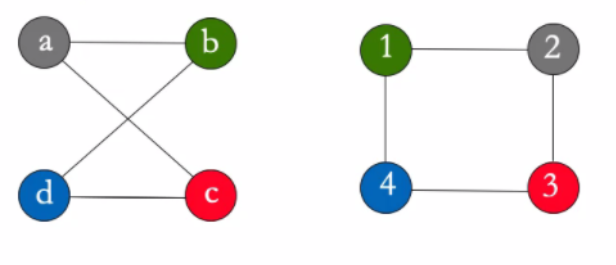
\includegraphics{./image/image-20201110233258123.png}

A questo punto però si crea un problema, infatti in alcuni casi, usando
un dato algoritmo ottengo risultati diversi se non qualifico un qualche
tipo di \textbf{parametro}. Proprio il concetto di parametro (inteso nel
senso informatico, cioè elemento che caratterizza un determinato
algoritmo e che l'algoritmo si aspetta per eseguire un compito). I
parametri quindi possono \textbf{condizionare l'esecuzione del task}.

\hypertarget{come-descrivere-un-algoritmo}{%
\subsubsection{Come descrivere un
algoritmo:}\label{come-descrivere-un-algoritmo}}

L'algoritmo per definizione è una sequenza precisa di passi, di
conseguenza una lista non ordinata di elementi non è l'oggetto giusto
per la sua rappresentazione. Inoltre il fatto che attraverso un
parametro si possa ottenere un risultato diverso rende la sua codifica
difficile.

Innanzitutto è essenziale che sia descritto come un programma, cioè come
una sequenza di istruzioni scritte in un linguaggio comprensibile al
calcolatore. Il compito del programmatore è proprio quello di scrivere
del codice che porti alla soluzione ottimale del problema.

Per iniziare bisogna inizialmente \textbf{definire esattamente il
problema}, che può essere:

\begin{enumerate}
\def\labelenumi{\arabic{enumi}.}
\tightlist
\item
  problema di \textbf{puro calcolo e conversione}, cioè risolvibile
  attraverso conoscenze matematiche.
\item
  problemi di \textbf{decisione}, cioè capire se una certa proprietà è
  propria di un certo elemento. (es. 15467 è primo?).
\item
  problemi di \textbf{ricerca}, cioè trovare un elemento con determinate
  caratteristiche in un determinato insieme.
\end{enumerate}

Il passaggio da definizione del problema a esecuzione del task poi passa
da altri step, che sono necessari alla codifica e alla comprensione dei
vari step:

\begin{enumerate}
\def\labelenumi{\arabic{enumi}.}
\tightlist
\item
  Problema: linguaggio \textbf{Lp}, ovvero linguaggio naturale (per
  descrivere il problema).
\item
  Algoritmo: linguaggio \textbf{La}, ovvero lo pseudocodice (lascia meno
  incomprensione ma più difficile da leggere).
\item
  Programma: linguaggio \textbf{Lt}, ovvero linguaggio macchina (es.
  C/C++).
\end{enumerate}

Una volta eseguiti questi \textbf{macropassaggi} si può passare alla
rifinitura del processo, attraverso dei \textbf{micro-algoritmi} (alcune
volte il programma e l'algoritmo necessario al suo funzionamento sono
così semplici da non necessitare la stesure di micro-algoritmi di
supporto).

Su algoritmi molto complessi si può applicare la tecnica del
\textbf{deconstruct}, ovvero decostruire il problema finché non si
ottengono tanti problemi di facile soluzione.

Nel caso della stesura di un algoritmo si devono prendere in
considerazione tutte le casistiche. Ad esempio se si scrive un algoritmo
per cercare un libro bisogna anche tenere in considerazione la
possibilità che questo libro non sia presente nell'indice della ricerca.
Allo stesso modo non si può pensare di avere una differenza abissale di
prestazioni se il libro è presente nella prima parte di indice o invece
è in fondo. Ci sono di solito sempre più di un modo per risolvere
problemi, quindi il problema principale diventa quello di trovare il
modo più efficiente disponibile.

\hypertarget{la-programmazione-e-il-linguaggio-di-programmazione}{%
\subsubsection{La programmazione e il linguaggio di
programmazione}\label{la-programmazione-e-il-linguaggio-di-programmazione}}

Programmare innanzitutto significa analizzare un problema, progettare un
algoritmo per ottenere una soluzione, esprimere l'algoritmo in un
linguaggio di programmazione, mettere la macchina nella situazione di
eseguire il programma e infine correggere eventuali errori.

L'algoritmo deve essere tradotto da linguaggio formale e reso
comprensibile all'esecutore. L'insieme dei comandi dati al calcolatore
in un certo linguaggio viene chiamato \textbf{programma}.

Il linguaggio di programmazione deve essere \textbf{rigoroso e preciso}
dal punto di vista di:

\begin{enumerate}
\def\labelenumi{\arabic{enumi}.}
\tightlist
\item
  \textbf{sintassi}: le regole che descrivono le stringhe di parole
  riconosciute dal linguaggio.
\item
  \textbf{semantica}: regole per l'interpretazione delle stringhe e che
  descrivono i processi computazionali dell'esecutore (o più
  semplicemente un errore logico nella stesura del programma, cioè un
  errore nella comprensione logica del programma). Questo errore è più
  difficile da individuare perché il compilatore non dà errore, ma i
  risultati saranno incoerenti.
\end{enumerate}

Parlando di linguaggi di programmazione, bisogna dire anche qualcosa
sull'astrazione del linguaggio:

\begin{enumerate}
\def\labelenumi{\arabic{enumi}.}
\item
  se il linguaggio è di bassissimo livello, quindi troppo vicino alla
  macchina è difficile programmare.
\item
  se il linguaggio è troppo di alto livello, quindi molto vicino al
  linguaggio del programmatore, i programmi diventano inefficienti.

  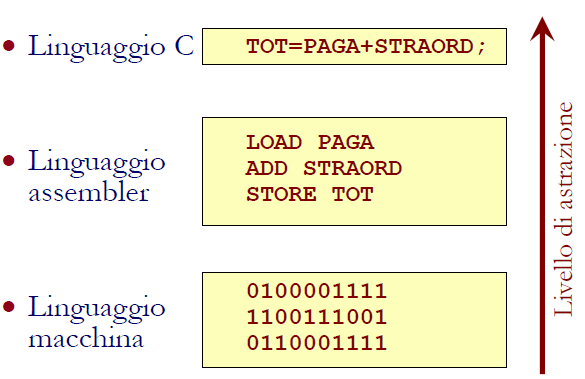
\includegraphics{./image/image-20201111001022024.png}
\end{enumerate}

Agli albori dell'informatica si programmava in linguaggio macchina, cioè
compreso direttamente dalla macchina.

Dagli anni '50 iniziano a nascere i primi linguaggi di programmazione di
alto livello, data la sempre più alta complessità dei programmi.

Ad oggi esistono tantissimi linguaggi di programmazione, ognuno con il
suo scopo e inventato per esigenze diverse.

\hypertarget{metodo-grafico-per-creare-algoritmi}{%
\subsubsection{Metodo grafico per creare
algoritmi:}\label{metodo-grafico-per-creare-algoritmi}}

Gli algoritmi possono essere schematizzati anche attraverso diagrammi di
flusso, cioè blocchi orientati che hanno un significato proprio.

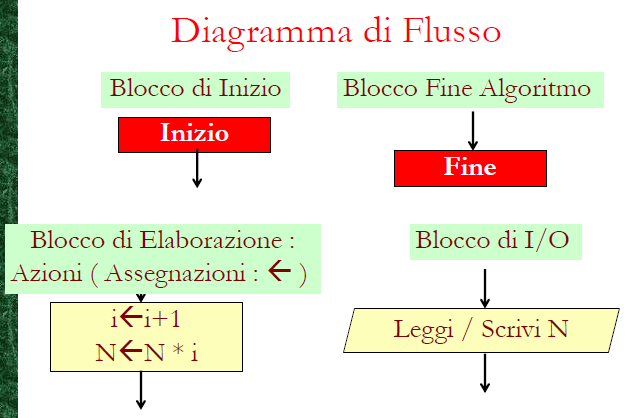
\includegraphics{./image/image-20201111002115408.png}

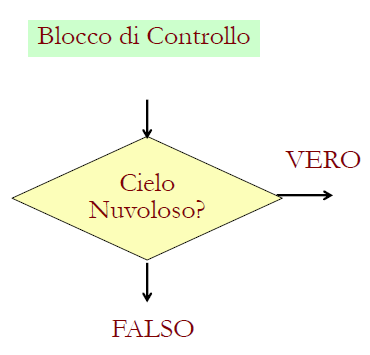
\includegraphics{./image/image-20201111002130617.png}

CARATTERISTICHE:

\begin{itemize}
\tightlist
\item
  BLOCCO \textbf{INIZIO}: unico nodo del grafo da cui si può solo
  partire infatti ha una sola freccia uscente. Rettangolo rosso per
  convenzione. Di solito si definisce con `1' l'inizio.
\item
  BLOCCO \textbf{FINE}: blocco in cui si può solo arrivare infatti ha
  una sola freccia entrante. Rettangoli rossi per convenzione. Di solito
  si definisce con `0' la fine.
\item
  BLOCCO \textbf{ISTRUZIONE}:

  \begin{itemize}
  \tightlist
  \item
    \textbf{assegnazione}: dà il valore che c'è a sinistra alla
    variabile di destra.
  \item
    \textbf{I/O}: (input/output), si sta leggendo o scrivendo
  \item
    \textbf{controllo}: (con più uscite, in questo caso vero e falso)
  \end{itemize}
\end{itemize}

\hypertarget{architettura-hardware-di-un-compilatore}{%
\subsection{Architettura hardware di un
compilatore:}\label{architettura-hardware-di-un-compilatore}}

\hypertarget{storia-del-calcolatore}{%
\subsubsection{Storia del Calcolatore:}\label{storia-del-calcolatore}}

Il primo calcolatore definito tale è ENIAC, creato nel 1945 in America
con il principale scopo di calcolare la traiettoria dell'artiglieria.
Poi donato al University of Pennsylvania, dove invece venne usato per il
calcolo ingegneristico e scientifico. Pesava circa 27 tonnellate e per
programmarlo erano necessarie diverse persone, infatti si basava su una
\emph{plugbboard} cioè un sistema di ``prese'' che, usate per fare il
contatto giusto, fornivano risultati alle operazioni date come input.
Non esisteva un linguaggio di programmazione pe questo computer e i
cosiddetti ``programmatori'' dell'epoca probabilmente non lo hanno mai
visto in tutta la loro vita, dato che loro facevano solo i calcoli per
farlo funzionare e poi qualcun altro si occupava di creare i giusti
collegamenti. La sua potenza di calcolo era tale da permettere di
calcolare quello che un uomo avrebbe fatto in 20 ore in soli 30 secondi.
Aveva un clock di circa 100kHz, e garantiva una vasta quantità di
calcoli possibili.

Dopo la seconda guerra mondiale inizia effettivamente lo sviluppo di una
macchina più vicina all'immaginari comune. Sempre più comuni diventano:

\begin{enumerate}
\def\labelenumi{\arabic{enumi}.}
\tightlist
\item
  MAINFRAME: computer di grandi dimensioni ed elevata potenza,
  solitamente condiviso fra più persone/uffici.
\item
  PERSONAL COMPUTER: computer dotati di tastiera e schermo separati, di
  memoria di massa interni o esterni alla memoria centrale e molto più
  economico.
\item
  LAPTOP: computer portatile, nonché evoluzione portabile del personal
  computer. Diventa molto famoso e utilizzato. Diventano così
  sofisticati che inizia il processo di miniaturizzazione dato che si
  poteva fare con le tecnologie disponibili ormai.
\item
  HANDHELD COMPUTER (SMARTPHONE): cellulari dotati di touchscreen, molto
  portabili e maneggevoli. Anche con questi come con i laptop avviene il
  processo di miniaturizzazione.
\item
  WHERABLE COMPUTER: sono computer così miniaturizzati da poter essere
  messi all'interno di un orologio, o un altro oggetto facilmente
  indossabile. Questi solamente sono caratterizzati da una gamma di
  sensori solitamente molto avanzati che possono servire per monitorare
  lo stato di salute o altri scopi.
\end{enumerate}

La miniaturizzazione che è avvenuta è dovuta alla possibilità di
dimezzare la grandezza del transistor per un certa quantità di volte,
data dalla legge di Moore.

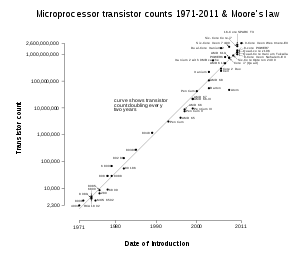
\includegraphics{./image/290px-Transistor_Count_and_Moore's_Law_-_2011.svg.png}

Moore infatti nel 1965 ipotizza che il numero di transistor inseribili
nei microprocessori sarebbe raddoppiato ogni anno. La sua previsione si
rivela corretta, finché verso la fine degli anni '80 viene riformulata:
raddoppio del numero di transistori ogni 18 mesi.

Per aumentare ancora più le prestazioni si cerca di aumentare il clock
dei processori stessi. Il \textbf{clock} di un processore è il dato che
indica la quantità di calcoli può fare al secondo. Al momento il dato
del clock è pressoché fermo intorno al dato di 3gHz. Questo stop è
dovuto al problema fisico per cui aumentando troppo il clock, il calore
emesso diventa esponenzialmente maggiore. Di conseguenza quando si sono
provati clock più alti si ha avuto problemi di gestione delle
temperature eccessivamente alte. Per ovviare questo problema si apre
un'altra strada: il multithreading o clock distribuito ad albero. Questo
permette di passare il clock in tutte le parti del processore e rendere
quindi i processi sincronizzati, utilizzando la potenza di tutte le
parti assieme e quindi garantendo una maggior potenza.

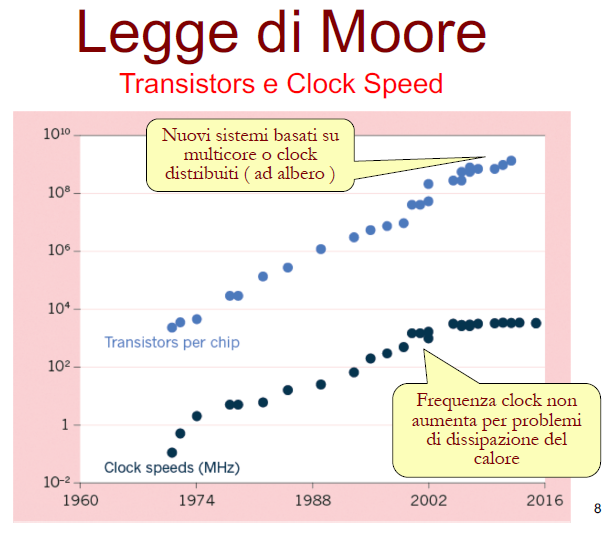
\includegraphics{./image/image-20201111171947392.png}

\hypertarget{organizzare-il-software-di-un-calcolatore}{%
\subsubsection{Organizzare il software di un
calcolatore}\label{organizzare-il-software-di-un-calcolatore}}

Il normale schema di un calcolatore è (generalmente) così costruito:

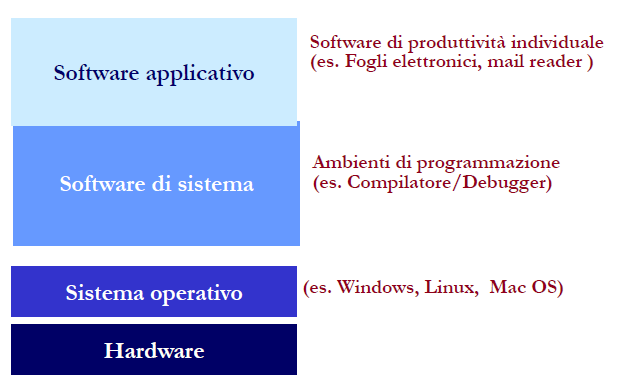
\includegraphics{./image/image-20201111172243268.png}

Per leggere questo schema bisogna capire che:

\begin{enumerate}
\def\labelenumi{\arabic{enumi}.}
\tightlist
\item
  Tutto si basa su quello che ha sotto di se e può comunicare solo con i
  blocchi a se adiacenti. (ad es. il software di sistema non si
  interfaccia direttamente con l'hardware, passa attraverso il sistema
  operativo).
\item
  L'unico che può operare con l'hardware è il sistema operativo. Questo
  ne gestisce tutte le componenti.
\end{enumerate}

\hypertarget{architettura-hardware}{%
\subsubsection{Architettura Hardware:}\label{architettura-hardware}}

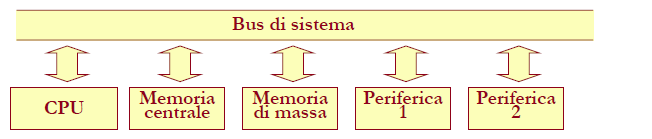
\includegraphics{./image/image-20201111172642835.png}

L'architettura hardware sopra è nota con il nome di \textbf{Macchina di
Von Neumann} ed è così costituita:

\begin{enumerate}
\def\labelenumi{\arabic{enumi}.}
\tightlist
\item
  \textbf{CPU} (central processing unit): svolge l'elaborazione
  eseguendo i programmi logici.
\item
  \textbf{MEMORIA CENTRALE }: memoria utilizzata per memorizzare dati e
  istruzioni, volatile (usata quindi solo per l'esecuzione di
  programmi).
\item
  \textbf{MEMORIA DI MASSA }: usata per memorizzare grandi quantità di
  dati e programmi in maniera persistente, al contrario della memoria
  centrale.
\item
  \textbf{PERIFERICHE}: sono di vario tipo e servono a tutto quello che
  permette l'interazione con il calcolatore. (ad es. tastiera, monitor,
  stampante, ..).
\item
  \textbf{BUS DI SISTEMA}: elemento che interconnette gli altri
  componenti consentendo lo scambio di dati, quindi anche il
  collegamento fra periferiche e hardware.
\end{enumerate}

\hypertarget{macchina-di-von-neumann}{%
\subsubsection{Macchina di Von Neumann:}\label{macchina-di-von-neumann}}

\hypertarget{cpu-unituxe0-di-elaborazione}{%
\paragraph{CPU: unità di
elaborazione}\label{cpu-unituxe0-di-elaborazione}}

La CPU è l'unità di elaborazione del calcolatore, si occupa di caricare
le istruzioni in memoria centrale, interpretarle e eseguirle.

E' altamente specializzata, perché è pensata per eseguire pochi tipi di
operazioni ma molto velocemente.

Il suo lavoro è scandito dal \textbf{clock} (orologio interno). La
potenza del calcolatore dipende in parte dal clock, infatti quanto più
questo è alto, tante più sono le istruzioni che riesce ad eseguire al
secondo. La sua frequenza infatti viene misurata in Hz, e 1 Hz = 1
ciclo/s. Ad oggi le CPU riescono a lavorare in parallelo, il cosiddetto
``lavoro condiviso'', grazie al clock. Infatti il segnale del clock che
arriva a tutti sincronizzato permette di eseguire azioni
contemporaneamente.

\hypertarget{memoria-centrale}{%
\paragraph{Memoria centrale:}\label{memoria-centrale}}

La memoria centrale è destinata a accogliere dati e programmi sui quali
opera il calcolatore. (ad es. quando usiamo il computer qui vengono
memorizzati i dati di programmi che stiamo usando, \ldots). La memoria
centrale è velocissima ma volatile (cioè una volta che il programma
finisce, tutti i dati di un programma vengono cancellati e lo spazio
viene liberato). Questa memoria accoglie i dati necessari a far
funzionare i programmi. Concettualmente è composta da una sequenza di
celle ognuna delle quali contiene una parola (\textbf{word}). Ad ogni
cella si può accedere direttamente specificandone l'\textbf{indirizzo},
e accedendone si può cambiare il suo contenuto (read/write). La quantità
di bit da cui è composta la word dipende dalla macchina, infatti è
caratteristico del microprocessore e attraverso questo si identifica lo
spazio di indirizzamento.

La memoria centrale solitamente è realizzata da una \textbf{RAM} (random
access memory). La sua caratteristica è che ogni cosa è accessibile e
non devo scansionare tutti gli indirizzi per cercare la cella che ho
bisogno. (per es. non è come il nastro magnetico che devono fisicamente
essere spostate avanti e indietro per trovare l'informazione cercata).
Questo ha ricadute dirette sul tempo di accesso, che è indipendente
dall'indirizzo della word che si vuole accedere. Questa è una memoria
volatile quindi i dati presenti qui sopra si perdono quando si spegne la
macchina. Esistono SRAM (static RAM), molto veloce, può contenere pochi
dati acceduti molto frequentemente, e DRAM (dynamic RAM) che contiene
più dati, ma più lentamente.

Altri tipi di memoria presenti sono le \textbf{ROM} (read-only memory).
Hanno caratteristiche simile alle RAM, hanno un accesso veloce ai dati
(ma non come quello delle RAM) e si tratta di \textbf{memorie
permanenti} su cui però non si può scrivere. Tipicamente son utilizzate
per memorizzare dati e programmi che servono prima del caricamento del
Sistema Operativo (ad es. per il caricamento del BIOS = Basic
Input-Output System).

La memoria quindi com'è fatta? Appare come una lista di word cioè un
mattoncino composto da 16bit, di conseguenza posso memorizzare tanti dai
quanti 2\^{}16 valori binari. All'interno della memoria ci posso mettere
tante word come gli indirizzi di memoria che sono 1024, e sono assegnati
da 0 a 1023. Se questi fossero i limiti del tuo microprocessore allora
devi fare in modo che all'interno di questo spazio di memoria ci stiano
i dati e i programmi necessari al tuo scopo.

Per questo motivo in memoria non si può accedere a valori più grandi di
2\^{}16 e non si può accedere all'indirizzo 1024.

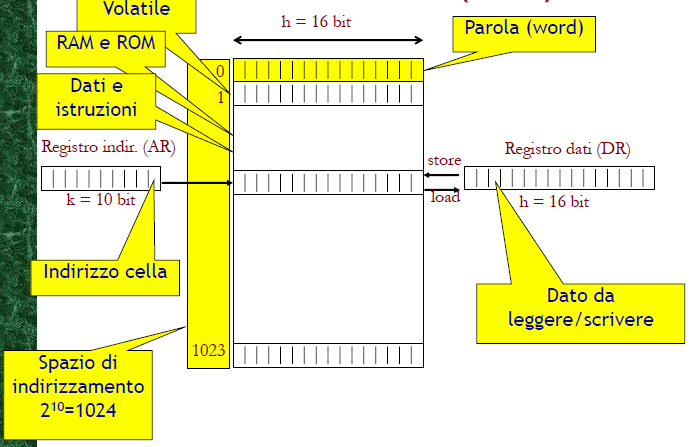
\includegraphics{./image/image-20201111185631084.png}

Però poi a questa memoria si deve poter accedere, quindi nella CPU
esistono dei registri, che sono word di memoria chiamate così per
distinguerle da quelle in memoria centrale. Questi registri possono
essere:

\begin{enumerate}
\def\labelenumi{\arabic{enumi}.}
\tightlist
\item
  AR (Address Register): di almeno 10 bit, perché in questo caso posso
  indirizzare da 0 a 1023
\item
  DR (data Register): posto in cui i dati di cui la CPU ha bisogno per
  fare operazioni che vengono copiati in questa posizione dalla memoria
  centrale per rendere le informazioni direttamente disponibili alla
  CPU.
\end{enumerate}

I registri sono elementi di supporto al calcolo.

\hypertarget{gerarchia-di-memoria}{%
\paragraph{Gerarchia di memoria}\label{gerarchia-di-memoria}}

Ci sono a disposizione memorie con caratteristiche diverse in base al
loro scopo:

\begin{enumerate}
\def\labelenumi{\arabic{enumi}.}
\tightlist
\item
  Registri: presenti nella CPU, piccoli ma veloci, utili per contenere
  dati temporanei per le operazioni della CPU
\item
  Memoria cache (SRAM): veloce, contiene pochi dati usati/richiesti
  frequentemente
\item
  Memoria principale (DRAM): meno veloce ma contiene più dati
\item
  Memoria secondaria o di Massa: molti dati, indicativamente più lenti
  (anche se gli SSD consentono un vantaggio prestazionale rispetto agli
  HD o agli HHD).
\end{enumerate}

\hypertarget{rappresentazione-dellinformazione}{%
\paragraph{Rappresentazione
dell'informazione:}\label{rappresentazione-dellinformazione}}

Tutti i dati vengono solitamente rappresentati in maniera
\textbf{binaria}, ovvero il bit che può prendere il valore 0 o 1. Questo
è molto utile perché si basano strutturalmente basati su dispositivi
bistabili (corrente ON o corrente OFF). Per questo l'elaboratore
elettronico può operare solo su sequenze di simboli binari.

Il BIT (derivato da Bynary digIT) è quindi l'unità elementare
dell'informazione. Comandi e dati nel computer vengono quindi
rappresentati con lunghe sequenze di numeri binari.

Essendo tutto codificabile attraverso il bit, allora sono state
inventate strutture per contenere la rappresentazione figurata della
realtà. Ad esempio la convenzione ASCII, poi diventata extended-ASCII,
ha codificato i caratteri come sequenza di 8bit, il \textbf{byte}.

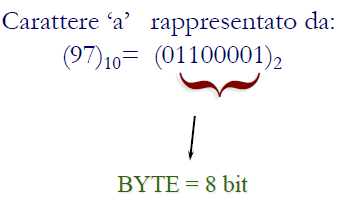
\includegraphics{./image/image-20201111184647324.png}

Per i multipli del byte si adottano gli stessi simboli del sistema
decimale, ma visto che gli elementi sono in base 2, il fattore di scala
è leggermente diverso:

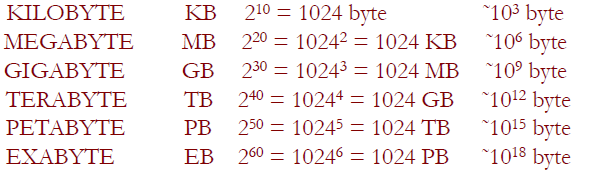
\includegraphics{./image/image-20201111184937248.png}

\hypertarget{funzionamento-della-cpu}{%
\paragraph{Funzionamento della CPU:}\label{funzionamento-della-cpu}}

Innanzitutto bisogna dire che:

\begin{enumerate}
\def\labelenumi{\arabic{enumi}.}
\tightlist
\item
  il trasferimento dei dati avviene con il bus di sistema.
\item
  Le fasi di elaborazione si susseguono in modo sincrono rispetto
  all'orologio di sistema (clock).
\item
  Durante ogni intervallo di tempo \textbf{l'unità di controllo} (che fa
  parte del processore) stabilisce la funzione da svolgere.
\item
  L'intera macchina opera in maniera sequenziale (però architetture più
  evolute prevedono l'esecuzione parallela delle istruzioni).
\end{enumerate}

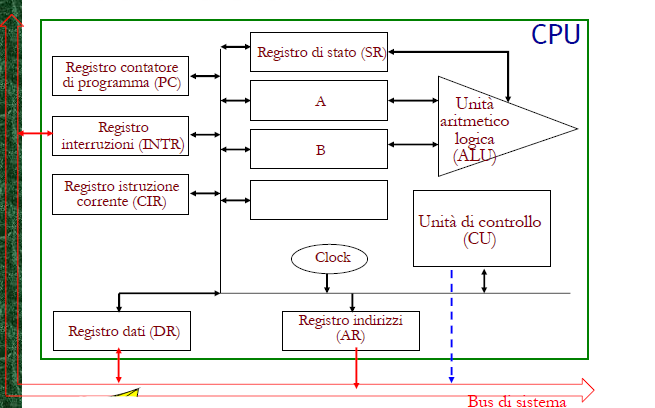
\includegraphics{./image/image-20201111191808017.png}

Come si vede dall'immagine la CPU ha a disposizione vari elementi:

\begin{enumerate}
\def\labelenumi{\arabic{enumi}.}
\tightlist
\item
  i registri (PC, INTR, CIR, DR, AR, \ldots)

  \begin{itemize}
  \tightlist
  \item
    registro di stato della CPU (\textbf{SR})(FLAG: C, Z, S, V), serve a
    far capire al compilatore lo stato delle periferiche e delle varie
    parti del compilatore stesso.
  \item
    Il program counter (\textbf{PC}) indica gli indirizzi dove andare a
    prendere la prossima istruzione.
  \item
    registro istruzioni (\textbf{INTR}) segnale lo stato di
    funzionamento delle periferiche.
  \end{itemize}
\item
  unità di controllo: capacità di controllare quello che sta succedendo,
  in pratica manda segnali per impartire degli ordini, in particolare
  possono provenire da questa unità il segnale di prelievo, di
  decodifica e d'esecuzione dell'istruzione.
\item
  Unità ALO: oggetto che esegue le operazioni aritmetico-logiche.
\item
  si nota il BUS di SISTEMA, responsabile di collegarsi ai vari registri
  e alle varie periferiche. (sotto)
\end{enumerate}

Il Ciclo base di funzionamento della CPU: (visione ad alto livello)

\begin{enumerate}
\def\labelenumi{\arabic{enumi}.}
\tightlist
\item
  FETCH

  \begin{enumerate}
  \def\labelenumii{\arabic{enumii}.}
  \tightlist
  \item
    La CU manda un segnale affinché il PC sia spostato nel AR (cioè la
    prossima istruzione viene indicizzata).
  \item
    segnale controllo (read) alla memoria centrale posto all'indirizzo
    in AR.
  \item
    il dato letto viene messo a disposizione nel DR (registro dei dati).
  \item
    la CU manda il segnale di controllo affinché il contenuto di DR sia
    spostato nel CIR (registro istruzione corrente).
  \end{enumerate}
\item
  INTERPRETAZIONE: le informazioni sul CIR vengono decodificate dalla
  CU.
\item
  ESECUZIONE: la CU genera una sequenza di segnali di controllo
  necessari a eseguire l'istruzione.
\item
  il PC viene incrementato per puntare alla prossima istruzione.
\end{enumerate}

Durante l'esecuzione la CPU può eseguire 3 macro-tipologie di
istruzioni:

\begin{enumerate}
\def\labelenumi{\arabic{enumi}.}
\tightlist
\item
  Istruzioni aritmetiche.
\item
  istruzioni di controllo.
\item
  istruzione di trasferimento dei dati (sia registro-registro, sia
  memoria-memoria, sia memoria-registro, sia registro-memoria).
\end{enumerate}

\hypertarget{il-bus-di-sistema}{%
\paragraph{Il Bus di Sistema}\label{il-bus-di-sistema}}

Il bus di sistema è l'elemento che interconnette le varie periferiche e
i vari elementi del calcolatore. In ogni istante il bus è dedicato al
collegare due unità, una che trasmette e una che riceve. Il processore
esegue il \emph{bus mastering}, ovvero seleziona le connessioni da
attivare e indica l'operazione da svolgere. Il bus è suddiviso in tre
insiemi di linee: \emph{bus dati}, \emph{bus indirizzi} e \emph{linee di
controllo} (quest'ultime trasportano informazioni relative alla modalità
di trasferimento e alla temporizzazione).

Il Bus di sistema ha l'organizzazione della comunicazione cosiddetta
\emph{master/slave}, ovvero ci sono parti (\emph{slave}) che devono
sempre ascoltarne altre (i \emph{master}). Generalmente il master è
l'elemento di controllo, nonché quello che manda i segnali di
esecuzione.

\hypertarget{le-periferiche-memorie-di-massa}{%
\paragraph{Le periferiche: memorie di
massa}\label{le-periferiche-memorie-di-massa}}

Con il termine memoria di massa ci si riferisce a un dispositivo di
memorizzazione permanente capace di contenere grosse quantità di dati.

Possono essere: fissi o rimovibili, ad accesso sequenziale o casuale,
dispositivi in sola lettura(RO), in lettura scrittura (RW), o WORM
(Write Once Read Many), dispositivi magnetici, ottici o
magnetico-ottici.

\begin{enumerate}
\def\labelenumi{\arabic{enumi}.}
\item
  HARD DISK

  Sfruttano le proprietà magnetiche di alcuni materiali (sostanze
  ferromagnetiche) di poter assumere a comando una certa direzione di
  magnetizzazione. A ciascuna direzione associa un simbolo binario. Sono
  costituiti da micro-celle magnetizzabili indipendentemente. La
  magnetizzazione è semipermanente, cioè rimane anche in assenza di
  mancanza di corrente ma può essere modificata.
\item
  MEMORIE DI MASSA: HDD

  Usa uno schema di memorizzazione creato in fase di formattazione di
  basso livello. Ogni superficie è divisa in tracce concentriche. I dati
  sono memorizzati in maniera sequenziale. Ogni traccia è divisa in
  settori. L'insieme delle tracce omologhe poste su diverse facce è
  detto cilindro.
\item
  SSD: MEMORIE ALLO STATO SOLIDI

  Accesso completamente elettronico (invece che elettromagnetico) ai
  dati. Al momento costi maggiori per unità di memoria. Permettono uno
  start-up immediato, latenza molto bassa e velocità di trasferimento
  circa un ordine di grandezza maggiore rispetto agli hard disk.
\item
  RAID

  Per aumentare le prestazioni dei sistemi a disco è possibile
  raggruppare più dischi in un sistema RAID (Redundant Array of
  Inexpensive Disk). Questo sistema suddivide i file in blocchi
  registrati su dischi diversi per aumentare le prestazioni (data
  striping). Questo sistema è anche utilizzato per incrementare
  l'affidabilità dei sistemi a disco attraverso un meccanismo di
  ridondanza.
\end{enumerate}

\hypertarget{linterfaccia-delle-periferiche}{%
\paragraph{L'interfaccia delle
Periferiche}\label{linterfaccia-delle-periferiche}}

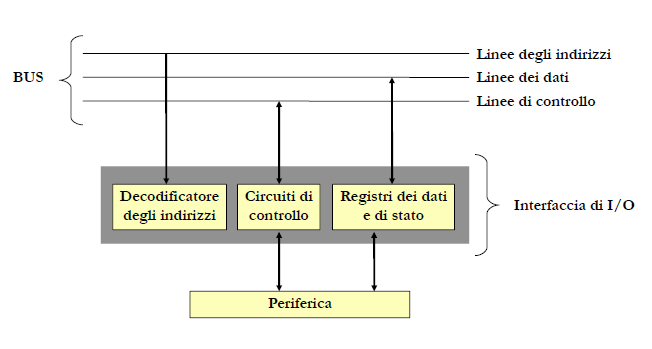
\includegraphics{./image/image-20201112230056001.png}

Comunicare con le periferiche può essere complicato, infatti se si
dovesse avere del codice per parlare con ogni singola periferica il
lavoro del programmatore diventerebbe impossibile. Per questo esiste
un'interfaccia, che fa come da traduttore tra il linguaggio della
periferica e la macchina.

E' possibile avere un interfaccia diversa per ogni periferica, ma è più
logico avere delle interfacce standard per periferiche simili. (Ad es.
USB: Universal Serial Bus).

Questa interfaccia si occupa concettualmente della gestione e dello
scambio di dati tra il processore e le periferiche. In generale
contiene:

\begin{enumerate}
\def\labelenumi{\arabic{enumi}.}
\tightlist
\item
  un registro dati della periferica
\item
  un registro di comando della periferica
\item
  un registro di stato (questo talvolta collegato al registro delle
  interruzioni del processore)
\end{enumerate}

A seconda del processore e dei registri delle periferiche, le interfacce
possono:

\begin{enumerate}
\def\labelenumi{\arabic{enumi}.}
\tightlist
\item
  condividere lo spazio di indirizzi della memoria (memory mapped I/O)
\item
  adottare uno spazio di istruzioni/indirizzi distinti (port mapped I/O)
\end{enumerate}

Le periferiche attraverso le interfacce possono essere gestite con due
metodi principalmente:

\begin{enumerate}
\def\labelenumi{\arabic{enumi}.}
\tightlist
\item
  POLLING: il processore invia sul bus il comando di lettura e si mette
  in attesa che il dato sia disponibile sul registro della periferica
  attraverso continui cicli. (PRO: facile implementazione e gestione;
  CONTRO: tiene sospeso il processore nel ciclo di attesa del dato).
\item
  INTERRUPT: il processore invia il comando di lettura alla periferica e
  poi continua le sue operazioni. Quando il dato è disponibile sul
  registro della periferica, la periferica stessa ``solleva'' un
  \emph{interrupt}, un interruzione. Il processore così interrompe le
  sue operazioni, salva il proprio stato ed esegue una opportuna routine
  per la gestione delle interruzione (compito del sistema operativo).
  Questa routine serve a verificare la presenza del dato sulla
  periferica del dato e a iniziare il trasferimento nel registro interni
  al processore, fino ad arrivare in memoria. Alla fine
  dell'\emph{interrupt} il processore ritorna alle sue operazioni
  normali. (PRO: lascia più libero il processore di operare; CONTRO:
  gestione, implementazione e controllo più complicati).
\end{enumerate}

Tra le periferiche sono presenti anche i terminali, cioè qualunque
dispositivo di puntamento (tastiera, mouse, video \ldots), e le
stampanti.

\hypertarget{architettura-software-di-un-compilatore}{%
\subsubsection{Architettura software di un
compilatore:}\label{architettura-software-di-un-compilatore}}

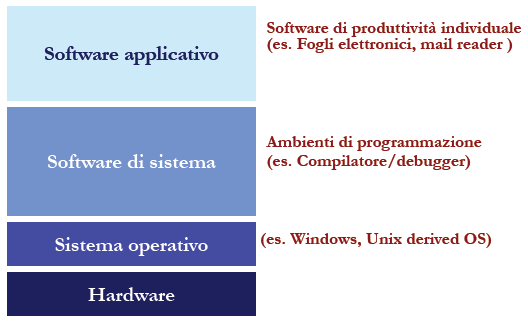
\includegraphics{./image/image-20201112231919938.png}

Con il termine \emph{sistema operativo} intendiamo l'insieme di
programmi che opera direttamente sulla macchina fisica, fornendo
interfacce di alto livello e mascherandone le caratteristiche specifiche
delle periferiche e del processore. Questo ad esempio è molto utile
nella gestione delle periferiche, perché permette di fornire un metodo
\emph{consistente} delle periferiche, ovvero una modalità standard di
interfacciarsi con le periferiche disponibili senza dover eseguire
comandi di basso livello. Importante notare inoltre che il sistema
operativo è l'unico elemento con accesso diretto alle risorse hardware,
e si riesce ad accedervi in altro modo direttamente probabilmente
abbiamo un problema.

Il sistema operativo è il modo che consente ai programmi di ottenere
risorse dal calcolatore. La traduzione da programma a calcolatore
avviene ad alto livello, in modo che non si debba scontrarsi con la
gestione degli indirizzi o dei registri. Il sistema operativo quindi,
dovendo gestire tutte le funzionalità di basso livello attraverso dei
controlli di alto livello, opera un alto livello di astrazione del
linguaggio macchina.

\hypertarget{storia-dei-sistemi-operativi}{%
\subsubsection{Storia dei sistemi
operativi:}\label{storia-dei-sistemi-operativi}}

Nel 1982 Kernigham introduce Unix, prodotto dai laboratori AT\&T, che al
tempo avevano grandi esigenze di un ecosistema stabile e uguale su cui
sviluppare applicazioni. Caratteristica principale: poteva servire più
utenti contemporaneamente, usando il multitasking. Tutti gli utenti
infatti hanno un ordine di esecuzione al processore, ma sono tutti
nell'ordine del proprio utente. Da Unix poi si svilupperanno tutti i
sistemi operativi che tuttora conosciamo (Come MS-DOS o Linux).

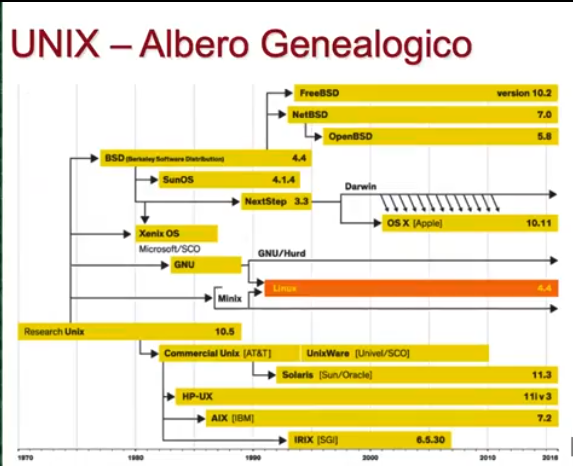
\includegraphics{./image/image-20200930171019756.png}

Architettura di un SO, che ad oggi è organizzato secondo un architettura
a \emph{strati} (anche detta \emph{onion skin architecture}). Ogni
strato fornisce un astrazione dello strato sui cui si appoggia e
permette una chiara separazione tra interfaccia e implementazione delle
diverse funzionalità, oltre che a fornire l'insieme di programmi e
librerie.

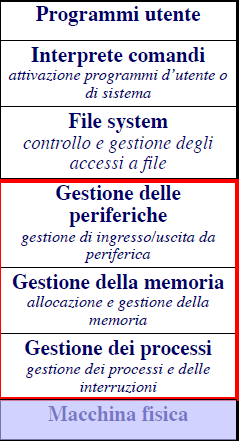
\includegraphics{./image/image-2020112323365770.png}

Il \emph{kernel} del sistema operativo, ovvero il cuore dell'OS si
occupa di:

\begin{itemize}
\tightlist
\item
  gestione periferiche (I/O informazioni)
\item
  gestione memoria (Fornisce/non fornisce al memoria in base al carico
  del momento, stabilisce il tipo di memoria da fornire)
\item
  gestione dei processi
\end{itemize}

Un processo è un entità dinamica, contrariamente al programma, infatti
viene causato dal codice in esecuzione (\emph{programma}) e dal suo
stato di esecuzione (es. valore delle sue variabili).

Un processo è quindi un insieme di due elementi:

\begin{itemize}
\tightlist
\item
  E: il codice eseguibile del programma (questo fa partire il fetch per
  creare un processo)
\item
  S: lo stato del processo
\end{itemize}

Logicamente il processo non viene gestito direttamente dal processore
reale, se no verrebbe meno il concetto di multitasking. Il processore
crea dei processori virtuali che si comportano similmente e che possono
essere assegnati a un processo.

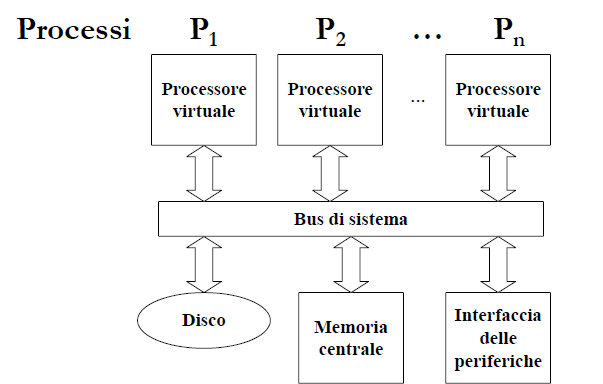
\includegraphics{./image/image-20201123234616173.png}

Nel processore è possibile che ci sia un solo processo in esecuzione in
ogni istante, mentre gli altri processi sono pronti o in attesa. Ad ogni
processo viene assegnato un valore massimo di tempo di esecuzione,
scaduto tale viene revocato il processore virtuale e assegnato a un
altro processo. Questa tecnica è detta di time-sharing, viene eseguito
dal nucleo che decide da quali processi devono andare in esecuzione
determinando lo \emph{scheduling}, che è sequenziale. La soluzione
tipica per la gestione del tempo di esecuzione di processi è a turno
(\emph{round-robin}, tutti i processi in questo hanno la stessa priorità
ad essere eseguiti, nella realtà non funziona perché alcuni processi
hanno la priorità). La CPU viene rilasciata anche quando un processo sta
aspettando un I/O da/verso una periferica.

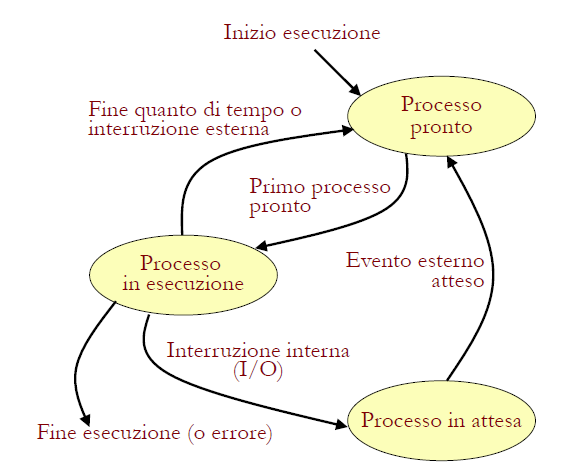
\includegraphics{./image/image-20201123235406308.png}x

In questa complicata gestione delle risorse prende parte anche la
gestione della memoria, che pensa al partizionamento della memoria tra i
vari processi che la richiedono garantendo la protezione/separazione fra
le diverse zone allocate. Il gestore memoria gestisce anche la memoria
che va assegnata ai processi, e quando i processi finisco la memoria
fisica si occupa di creare una memoria virtuale (più lenta di solito,
chiamata SWAP o semplicemente memoria virtuale) e assegnare quella
memoria.

\hypertarget{the-c-programming-language}{%
\section{THE C PROGRAMMING LANGUAGE:}\label{the-c-programming-language}}

Ci sono principalmente 3 tipi di programmazione:

\begin{itemize}
\tightlist
\item
  programmazione per HARDWARE, ovvero la programmazione di dispositivi
  fisico/logici il cui il linguaggio di programmazione coincide con il
  linguaggio macchina.
\item
  programmazione per FIRMWARE, ovvero la programmazione che usa
  un'insieme comune di istruzioni mediante assembly, ovvero linguaggio
  di programmazione molto basso
\item
  programmazione per SOFTWARE, ovvero programmare in un linguaggio
  intermedio che simula le funzionalità della macchina fisica, che per
  questo permette maggiore flessibilità (nel senso che posso realizzare
  un gran numero di programmi diversi e con funzioni diverse), ma che ha
  un utilizzo delle risorse meno efficiente.
\end{itemize}

Il sistema operativo prende parte molto nell'ultimo caso, infatti è suo
il compito di fornirci le periferiche necessarie a fornire la traduzione
da linguaggio macchina (che usano ad esempio nella programmazione
firmware) e il codice. L'OS si occupa anche dell'astrazione degli
oggetti e/o delle istruzioni complesse di alto livello.

\hypertarget{diffusione-dei-linguaggi-e-perchuxe9-il-c}{%
\subsection{Diffusione dei linguaggi e Perché il
C}\label{diffusione-dei-linguaggi-e-perchuxe9-il-c}}

Ci sono tantissimi linguaggi di programmazione creati o utilizzati per
specifici utilizzi in cui sono molto apprezzati. Linguaggi più standard
di medio-basso livello come il C o il C++ permettono una maggior
comprensione del funzionamento della maggior parte degli altri
linguaggi, che in alcuni casi forniscono astrazioni alle strutture di
basso livello ancora presenti in questi.

Il C presenta una serie di elementi che lo rendono importante da
imparare:

\begin{itemize}
\tightlist
\item
  permette l'allocazione dinamica e altri aspetti normalmente di alto
  livello, a un livello basso.
\item
  gestione della memoria molto manuale
\item
  linguaggio apprezzato/richiesto dalle aziende
\item
  ha un astrazione che è posizionata tra il medio e il basso livello,
  motivo per cui è molto utile per ad. es. embedded system.
\end{itemize}

Il linguaggio C è stato creato nel 1972 da Kernighan e Ritchie ai Bell
Tel. Labs.

\hypertarget{operazioni-logiche-algebra-di-boole}{%
\subsection{Operazioni Logiche (algebra di
Boole)}\label{operazioni-logiche-algebra-di-boole}}

L'algebra di Boole è basata su tre operatori logici (NOT, AND, OR). Gli
operandi posso assumere due valori: VERO e FALSO.

Gli operatori godono della proprietà

\begin{itemize}
\tightlist
\item
  commutativa (es. A OR B = B OR A)
\item
  distributiva (es. A AND (B OR C) = (A AND B) OR (A AND C))
\end{itemize}

Le tabelle di verità associano a tutti i possibili valori degli operandi
il risultato

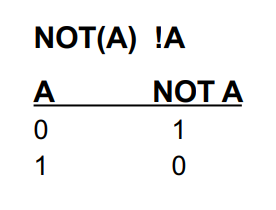
\includegraphics{./image/image-20201207220212631-1607774144622.png}

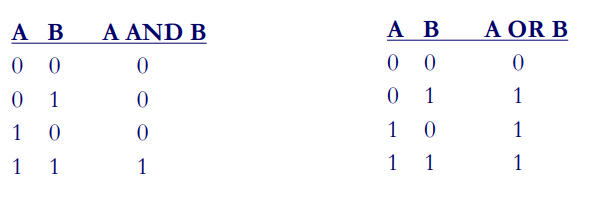
\includegraphics{./image/image-20201207220252086-1607774220882.png}

solitamente NOT viene rappresentata con !, AND con \&\& e OR con
\textbar\textbar.

quando si valuta un espressione l'ordine è il seguente (NOT, AND, OR),
per esempio.

\begin{figure}
\centering
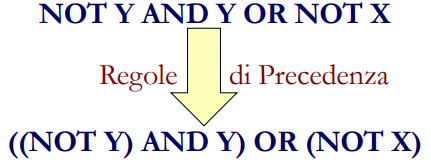
\includegraphics{C:/Users/giova/Documents/1_UNI/programmazione1/appunti/appunti-prog1/image/image-20201207220627893.png}
\caption{image-20201207220627893}
\end{figure}

Per calcolare il risultato di un espressione (per esempio NOT Y AND (Y
OR NOT X)) si crea una tabella di verità, prima con i valori singoli per
poi raggrupparli fino ad arrivare alla formula di partenza.

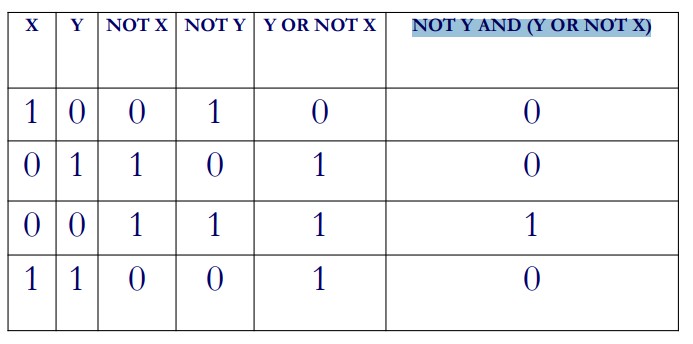
\includegraphics{./image/image-20201207220834575.png}

\hypertarget{leggi-di-de-morgan}{%
\subsubsection{Leggi di De Morgan}\label{leggi-di-de-morgan}}

\begin{itemize}
\tightlist
\item
  A AND B = NOT ((NOT A) OR (NOT B))
\item
  A OR B = NOT ((NOT A) AND (NOTB))
\end{itemize}

si possono dimostrare compilando la tabella di verità e osservando che
le tabelle delle espressione ai due lati dell'uguale hanno stessi
risultati a parità di input.

\textbf{Tautologia}: espressione che è sempre vera

\textbf{Contradizione}: espressione sempre falsa

\hypertarget{codifica-semplici-algoritmi-in-c}{%
\subsection{Codifica Semplici Algoritmi in
C}\label{codifica-semplici-algoritmi-in-c}}

istruzione di assegnamento:

\begin{lstlisting}[language={C++}]
x = 23;
w = 'a';
y = z;
\end{lstlisting}

\hypertarget{costruttore-if-else}{%
\subsubsection{Costruttore if-else}\label{costruttore-if-else}}

diagramma di flusso:

L'espressione tra parentesi viene valutata, se vera viene eseguito il
primo blocco, se falsa l'altro. Naturalmente si può utilizzare anche l'
if da solo senza else. All'interno dell'espressione posso utilizzare gli
operatori logici (\&\&, \textbar\textbar).

è sempre meglio utilizzare indentazione e paretesi graffe per una
migliore leggibilità e per non commettere errori.

**Operatore ternario \passthrough{\lstinline!?!}* *è un altro modo di
scrivere if-else, la sintassi è la seguente

\begin{lstlisting}[language={C++}]
espressione1 ? espressione2 : espressione3; //questo equivale al seguente if-else

if (espressione1)
    { espressione2; }
else
    { espressione3; }
\end{lstlisting}

dopo le parentesi graffe il ; non è necessario, ma se viene messo non
c'è errore.

\hypertarget{precedenza-degli-operatori}{%
\subsubsection{Precedenza degli
operatori}\label{precedenza-degli-operatori}}

In un espressione vengono eseguiti prima gli operatori con precedenza
superiore, se gli operatori sono dello stesso gruppo si usano le regole
di associatività (da destra o da sinistra), le parentesi posso essere
usate per modificare la precedenza.

Associatività da sinistra a destra significa che a parità di priorità
l'espressione viene eseguita partendo da sinistra a destra.

\begin{lstlisting}[language={C++}]
if (a + b - 4 <= 9 && x < tot - 1) // questa espressione è equivalente a quella sotto

if (((a + b - 4 <= 9) && (x < tot - 1 ) )
\end{lstlisting}

\hypertarget{istruzione-iterativa-ciclo}{%
\subsubsection{Istruzione Iterativa ( ciclo
)}\label{istruzione-iterativa-ciclo}}

il diagramma di flusso è il seguente (il ciclo si chiama while). Il
blocco istruzioni viene ripetuto fino a quando l'espressione non diventa
falsa.

(da pagina 38 a 56 un po' di esercizi noiosi)

\hypertarget{getchar-e-putchar}{%
\subsubsection{Getchar e Putchar}\label{getchar-e-putchar}}

\begin{lstlisting}[language={C++}]
//getchar legge il prossimo carattere inserito da tastiera
c = getchar();
//putchar stampa il carattere nello standard output
putchar(c)
\end{lstlisting}

\hypertarget{esercizio-scale}{%
\subparagraph{Esercizio scale:}\label{esercizio-scale}}

Sia data una scala di N gradini. Si supponga di salire l'intera scala
con passi da 1 , 2 o 3 scalini. In quanti possibili modi si può salire
l'intera scala ?

\textbf{risoluzione in modo semplice:}

Devo capire in quanti modi possibili posso salire una scala con n
gradini. Posso compiere passi da 1, 2 o 3 gradini.

Mi calcolo in quanti modi posso salire una scala formata da 1 2 o 3
gradini e basta.

Un gradino = 1 modo

Due gradino = 2 modo

Tre gradino = 4 modo

Per arrivare al quarto gradino ho solo tre possibilità: fare un passo da
uno, da due o da tre, quindi devo arrivare al gradino 4-1, 4-2, 4-3,
siccome so già quanti passi ci vogliono per arrivare in questi posti,
basta sommarli assieme per capire il numero di passi per arrivare al
quarto.

Aggiorno il numero di passi per il gradino n-1, n-2, n-3 e vado avanti.
(se non si capisce chiedetemi che vi spiego meglio).

\hypertarget{strutture-di-controllo}{%
\subsubsection{Strutture di controllo}\label{strutture-di-controllo}}

\hypertarget{istruzione-di-ciclo-for}{%
\paragraph{\texorpdfstring{Istruzione di ciclo:
\texttt{FOR}}{Istruzione di ciclo: FOR}}\label{istruzione-di-ciclo-for}}

schema a blocchi e sintassi:

questo operatore è utile quando so a priori quante operazioni devo fare,
in quei casi è più compatto rispetto ad un while.

\hypertarget{il-costrutto-do-while}{%
\paragraph{\texorpdfstring{Il costrutto
\texttt{DO-WHILE}}{Il costrutto DO-WHILE}}\label{il-costrutto-do-while}}

schema a blocchi e sintassi:

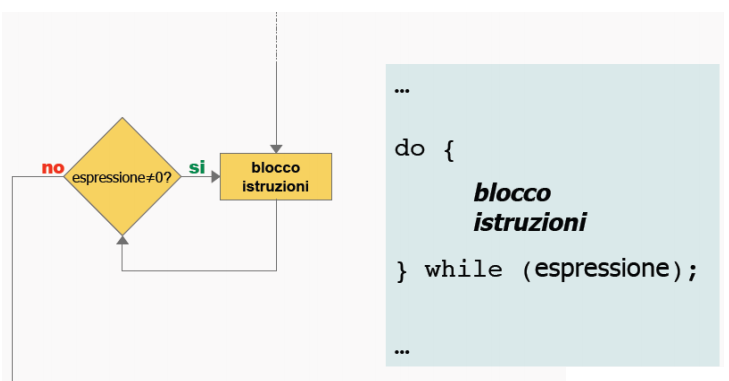
\includegraphics{./image/image-20201207224157049.png}

\begin{lstlisting}[language={C++}]
// un esempio
Contatore = 0;
do
{
    scanf (" %c", &Dato);
    Contatore ++;
} while (Dato != `\%');
\end{lstlisting}

si utilizza quando voglio eseguire un blocco di istruzioni almeno una
volta, può essere utile quando devo fare un controllo sull'input da
tastiera.

\hypertarget{il-costrutto-swith}{%
\paragraph{\texorpdfstring{Il costrutto
\texttt{SWITH}}{Il costrutto SWITH}}\label{il-costrutto-swith}}

Va a sostituire un if-else multiplo, schema a blocchi e sintassi:

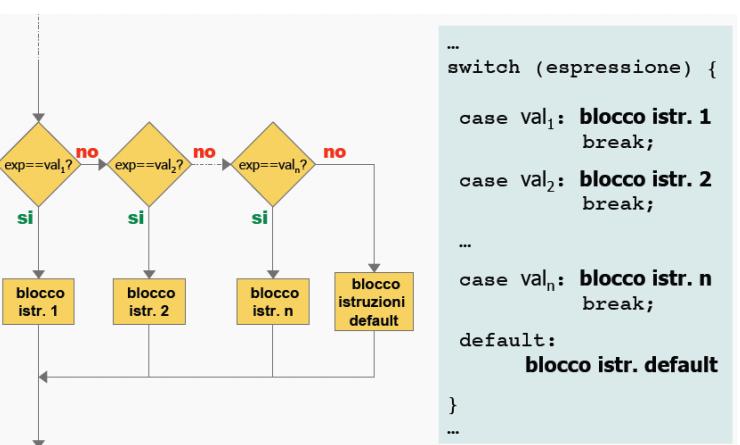
\includegraphics{./image/image-20201207224317378.png}

Il \textbf{default} (le istruzioni che vengono eseguite in caso che
nessuna delle altre sia vera) è opzionale. I singoli case vengono
eseguiti quando il valore dell'espressione è uguale a quello scritto
appena dopo l'istruzione case. ATTENZIONE: bisogna mettere il break dopo
il blocco istruzioni altrimenti si rimane all'interno dello switch
(verranno valutati i case seguenti ed eseguito il default se presente).

Valuta solo variabili di tipo INT, quindi l'espressione deve avere come
risultato un int.

\textbf{Break}: quando viene eseguito all'interno di un while, for, do,
switch provoca l'uscita dall'istruzione

\textbf{Continue}: quando viene eseguito all'interno di un ciclo passa
alla iterazione successiva

un linguaggio di programmazione può codificare qualsiasi algoritmo se
ha: sequenza di istruzioni, if-else e while.

\hypertarget{array-in-c}{%
\subsection{Array in C}\label{array-in-c}}

Gli array possono essere paragonati a vettori e matrici in matematica.
Da un punto di vista più concreto sono una sequenza di celle di memoria
consecutive e omogenee. L'array è quindi un contenitore per
\emph{variabili dello stesso tipo}.

A ciascun elemento dell'array si accede tramite indice (esempio a{[}i{]}
è l'elemento alla posizione i-esima). Le parentesi quadre sono operatori
ad alta precedenza (sono al primo livello della tabella).

Il primo elemento dell'array è quello in posizione 0, la macchina
astratta prende l'indice e lo somma all'indirizzo della prima cella
dell'array.

Prima di utilizzare le array bisogna dichiararle:

\begin{lstlisting}[language={C++}]
int a[100]; // dichiara un contenitore a (array) che potrà contenere 100 elementi di tipo int, il primo elemento lo si trova in a[0], l'ultimo in a[99]
\end{lstlisting}

il compilatore va a riservare la memoria per tutti questi elementi

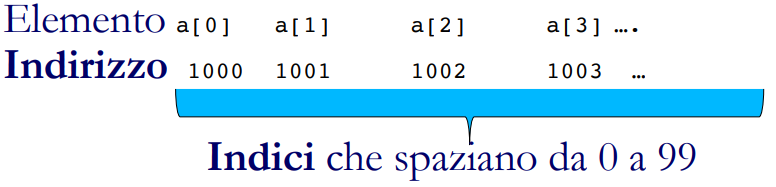
\includegraphics{./image/image-20201208144533768-1607774562526.png}

In generale l'ultimo elemento dell'array è nella posizione n-1, dove n è
la lunghezza dell'array stessa. All'interno delle parentesi si possono
mettere delle espressioni. Un veloce esercizio:

SOLUZIONE: a{[}0{]}= indeterminato, a{[}1{]} = 6

ATTENZIONE: se vado oltre l'indice massimo dell'array accedo a celle di
memoria che non appartengono all'array e il cui valore è indeterminato.

L'array in C non è un tipo, ma un costruttore di tipo.

\hypertarget{inizializzazione-e-stampa}{%
\subsubsection{Inizializzazione e
stampa}\label{inizializzazione-e-stampa}}

si può inizializzare direttamente al momento della dichiarazione

\begin{lstlisting}[language={C++}]
int a[5] = {5, 2, -5, 10, 234};
int b[4] = {5, 2, -5}; //un elemento non è inizializzato
int c[2] = {5, 2, -5}; // ERRORE: inizializzato un elemento che non appartiene all'array
\end{lstlisting}

per array grandi questo metodo diventa scomodo, quindi si usano i cicli
per inizializzare.

anche per stampare un array devo utilizzare un ciclo

\begin{lstlisting}[language={C++}]
printf("%d", a); // errato perchè a è un array

int i=0; // questo è il procedimento corretto
while (i<5){
    printf("%d",a[i]);
    i++;
} 
\end{lstlisting}

esercizi sulle array dalla slide 31 a 41.

\textbf{Array dinamici}: il C permette inizializzare la dimensione di un
array durante l'esecuzione di un programma (per esempio chiedendo la
dimensione da tastiera).

\hypertarget{array-multidimensionali}{%
\subsubsection{Array multidimensionali}\label{array-multidimensionali}}

Le array di due dimensioni corrispondo alle matrici in matematica. Si
dichiarano nel seguente modo:

\begin{lstlisting}[language={C++}]
int a[N][M]; //N numero righe M numero colonne

//è anche possibile definire più dimensioni
int a[10][5][20];
\end{lstlisting}

Come per gli array ad 1 dimensione, anche questi possono essere
inizializzati nella fase di dichiarazione:

\begin{lstlisting}[language={C++}]
int a[4][5]= { {2, 5, -8, 7, 6},
                {3, 10, 7, 6, 1},
                {-1,8, -8, 5, 3},
                {2, 5, 8, 4, 2}
             };
\end{lstlisting}

Per semplicità possiamo immaginare l'array in due o più dimensioni, ma
la macchina astratta del C memorizza gli elementi uno dietro l'altro.
Per esempio l'array creata sopra verrà memorizzata nel seguente modo:

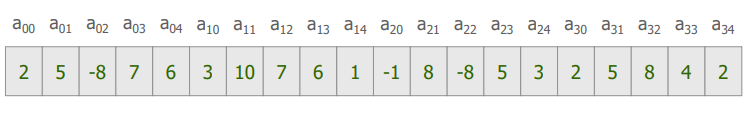
\includegraphics{./image/image-20201208150630550.png}

altri esempi di inizializzazione corretta e sbagliata:

\begin{lstlisting}[language={C++}]
int D[][]={1,2,3,4}; // errata
int E[2][]={1,2,3,4}; //errore non viene specificato il numero di colonne

int F[][4]={{1,2,3,4}}; //va bene 
// in c nella dichiarazione di un array bisogna valorizzare tutte le dimensioni, si può fare a meno di quella più a sinistra 
\end{lstlisting}

le array possono anche essere inizializzate con dei cicli

\begin{lstlisting}[language={C++}]
int main(int argc, char *argv[]){
    int matrice[10][5];
    int i=0,j=0;
    while (i<10)
    {
        j=0;
        while (j<5)
        {
            printf("%d ",matrice[i][j]);
            j++;
        }
        printf("\n");
        i++;
    }
}
\end{lstlisting}

esercizi da pagina 61 in poi

\hypertarget{stringhe-in-c}{%
\subsection{Stringhe in C}\label{stringhe-in-c}}

Un array di char può essere rappresentata con una stringa (per esempio
``hello''). L'ultimo carattere deve essere il carattere nullo
`\textbackslash0'. Questo carattere serve alle varie funzioni per capire
dove terminerà la stringa. Quindi quando vado a creare una stringa per
memorizzare n caratteri ne serviranno n+1 (uno lo uso per il carattere
nullo).

Esiste un modo semplificato per inizializzare un'array di caratteri come
stringa:

\begin{lstlisting}[language={C++}]
char mia_stringa[] = “Ciao a tutti!”;
\end{lstlisting}

Questo mi memorizza automaticamente lo spazio per il miei caratteri più
il carattere terminatore. Quindi il risultato sarà:

\begin{figure}
\centering
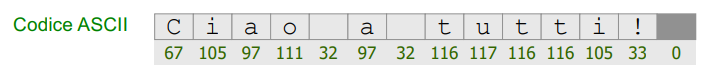
\includegraphics{C:/Users/giova/Documents/1_UNI/programmazione1/appunti/appunti-prog1/image/image-20201212103116117.png}
\caption{image-20201212103116117}
\end{figure}

L'inizializzazione vista sopra è molto più veloce ed è equivalente ad
inizializzare nel seguente modo:

\begin{lstlisting}[language={C++}]
char mia_stringa[] = {‘C’,‘i’,‘a’,’o’,’ ‘,’a’,’ ‘,’t’,’u’,’t’,’t’,’i’,’!’,’\\0’};
\end{lstlisting}

Se non specifico il numero all'interno delle parentesi quadre quando
dichiaro l'array il compilatore va a riservare uno spazio pari al numero
degli elementi con cui l'array viene inizializzato. Nel caso delle
stringhe posso anche dichiarare esplicitamente la dimensione di memoria
da riservare:

\begin{lstlisting}[language={C++}]
char frase[20]=”Ciao a tutti!”;
\end{lstlisting}

Bisogna stare attenti che un elemento (dei 20 messi a disposizione per
l'array) sarà occupato da `\textbackslash0' e poi gli elementi in più
saranno lasciati vuoti.

ATTENZIONE: se non specifico né il numero di caratteri (all'interno
delle parentesi quadre) né assegno alla stringa un valore, il
compilatore da un errore, perché non sa quanta memoria riservare.

\begin{lstlisting}
char parola[]; // ERRORE
\end{lstlisting}

per stampa le stringhe si usa \%s:

\begin{lstlisting}[language={C++}]
printf(“%s”, mia_stringa); //questo non sarebbe possibile se non ci fosse il carattere terminatore perché non saprei dove fermarmi 
\end{lstlisting}

quando faccio scanf non bisogna mettere la \& perché la stringa è un
array e la variabile con il suo nome è già un indirizzo.

\begin{lstlisting}[language={C++}]
scanf(“%s”, parola);
\end{lstlisting}

\hypertarget{rappresentazione-di-informazioni}{%
\subsection{Rappresentazione di
informazioni}\label{rappresentazione-di-informazioni}}

in un calcolatore le informazioni vengono rappresentate sotto forma di
dati, codificati in un linguaggio comprensibile al calcolatore. Per
permetterci di interpretare le informazioni i dati devono essere
decodificati. Quindi ci sono diversi livelli di decodifica che partono
dall'hardware fino ad arrivare ad informazioni interpretabili a noi
umani.

I tipi di dato che il calcolatore può interpretare direttamente sono :

\begin{itemize}
\tightlist
\item
  booleani
\item
  numeri interi
\item
  numeri frazionari
\item
  caratteri
\end{itemize}

Per questi dati la codifica è gestita direttamente dall'HW, per tipi di
dato più complessi si usa una rappresentazione di tipo software.

\hypertarget{interi}{%
\subsubsection{Interi}\label{interi}}

Sono rappresentati da una sequenza finita di bit. 8 bit (un byte)
permettono di rappresentare i valori da 0 a 255. Solitamente per gli
interi positivi si usano 4 byte (32 bit), quindi i numeri vanno da 0 a
4.294.967.295. (questo implica che all'interno dei calcolatori i numeri
sono finiti).

Per rappresentare anche i numeri negativi, si utilizza il primo bit come
bit di segno (0 per i numeri negativi, 1 per i positivi)

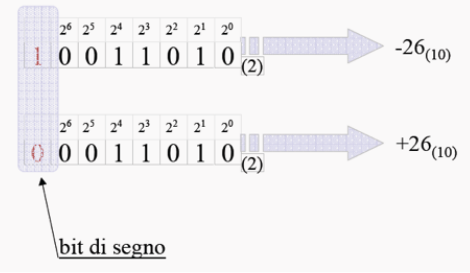
\includegraphics{./image/image-20201212110945997.png}

In realtà nei calcolatori non si usa questa rappresentazione ma quella
in complemento a due con i seguenti vantaggi: non c'è un doppio zero,
non c'è bisogno di una circuiteria specifica. Esempio:

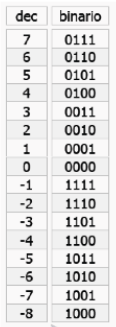
\includegraphics{./image/image-20201212111232217.png}

Per decodificare i valori positivi si procede nel modo normale, per
quelli negativi si decodifica e poi si sottrae 2\^{}N-1. Per invertire i
numeri si invertono gli zeri con gli uno e si somma uno.

\hypertarget{numeri-frazionari}{%
\paragraph{Numeri frazionari}\label{numeri-frazionari}}

I dati con numeri dopo la virgola vanno rappresentati in maniera
opportuna, ci sono due tecniche:

\begin{itemize}
\tightlist
\item
  \textbf{virgola fissa}: si dividono i bit che rappresentano i valori
  interi da quello per i valori dopo la virgola
\item
  \textbf{virgola mobile}: la maggior parte dei bit viene usata per le
  cifre rappresentative del numero, gli altri per sapere dove mettere la
  virgola.
\end{itemize}

esempio codifica virgola fissa:

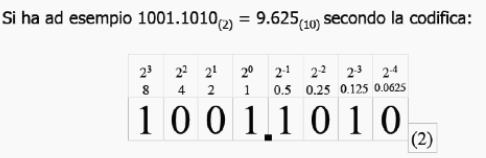
\includegraphics{./image/image-20201212112345743.png}

Per la virgola mobile solitamente vengono utilizzati 32 bit, 1 per il
segno, 8 per l'esponente e il resto per la mantissa

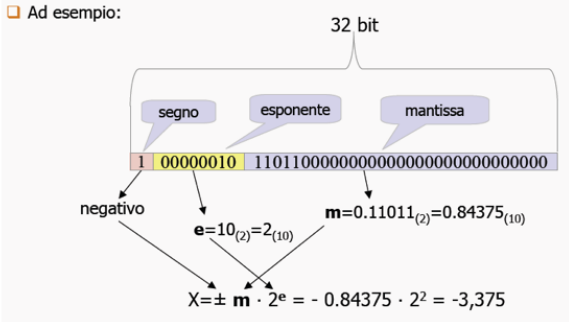
\includegraphics{./image/image-20201212112608865.png}

Quindi la mantissa rappresenta numeri da 0 a 1, che verranno
moltiplicati per 2\^{}e in modo da ottenere il numero desiderato. \[
m=0.11011_{(2)} =  2^{-1}+2^{-2}+2^{-4}+2^{-5} = 0.84375
\] un numero si dice normalizzato se l'esponente è diverso da 0, la
mantissa è compresa tra 1 e 2 l'intervallo dei numeri è \[
(-2^{128}, -2^{-126}][2^{-126}, 2^{128})
\]

\hypertarget{caratteri}{%
\subsubsection{Caratteri}\label{caratteri}}

per codificare i caratteri si utilizza la tabella ASCII, i primi 128
valori sono fissi i successivi rappresentato la tabella ASCII estesa con
caratteri più specifici (per esempio c'è una tabella ASCII estesa con i
caratteri è, ò, à\ldots).

attualmente si utilizza l'UNICODE che utilizza 2 bytes per ogni
carattere e permette di non avere tabelle diverse per ogni regione del
mondo.

\hypertarget{conversione-di-basi}{%
\subsubsection{Conversione di Basi}\label{conversione-di-basi}}

Come si fa a cambiare da base Esa a Ottale? Prima trasformo in binario e
poi in ottale, infine l'ultimo bit lo attacco agli altri gruppi in modo
da creare dei gruppi di bit tutti da 3.

\begin{figure}
\centering
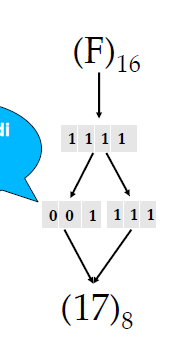
\includegraphics{C:/Users/giova/Documents/1_UNI/programmazione1/appunti/appunti-prog1/image/image-20201015154501158-1608629092098.png}
\caption{image-20201015154501158}
\end{figure}

Raggruppo fino a che posso, poi aggiungo zero. in questa maniera riesco
sempre a costruire triplette.

\begin{figure}
\centering
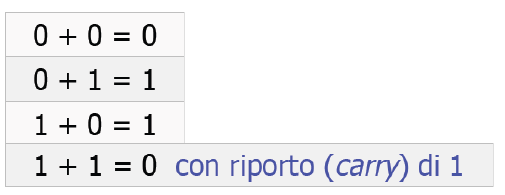
\includegraphics{C:/Users/giova/Documents/1_UNI/programmazione1/appunti/appunti-prog1/image/image-2020101515472845.png}
\caption{image-20201015154728645}
\end{figure}

\hypertarget{tipi-di-dato}{%
\subsubsection{Tipi di Dato}\label{tipi-di-dato}}

Il tipo di dato è un insieme di valori che può assumere una variabile, i
cui elementi possono fare operazioni esserne l'oggetto. In base
all'oggetto di cui ho bisogno e in base alle operazioni che devo
eseguire con quei dati allora dichiaro tipo di dati diversi, in base
allo scopo e alla funzione.

Classificazione:

\begin{itemize}
\tightlist
\item
  \textbf{built-in} (predefiniti): interi, caratteri, tipi strutturati
  (array o struct), etc.
\item
  \textbf{user-defined: }definiti dal programmatore, creati a piacere
  per uno scopo preciso.
\item
  ogni linguaggio offre diversi tipi di dati che possono essere
  predefiniti o semplici.
\end{itemize}

I tipi sono necessari per interpretare una serie di bit in memoria, e in
base al quale il compilatore o calcolatore lo traduce. Questa è un
operazione necessaria per l'utente finale che ha bisogno di un
astrazione, ma poco utile a bassissimo livello, infatti tutte le
informazioni sono codificate in binario. In secondo luogo i tipi sono
importanti anche perché permettono di comunicare quanta memoria si
necessita, e quindi quanta e che richiesta di memoria posso fare.

Un lato positivo di questi tipi di dato è che possono catturare qualche
errore logico, senza causare problemi durante l'esecuzione(ad esempio se
il tipo ha dei parametri che vengono utilizzati nel modo sbagliato è più
facile trovare l'errore dopo, ma allo stesso modo è più facile evitarlo
direttamente). Poi per il fatto che il linguaggio C è statically typed,
allora se si utilizza un oggetto come una cosa diversa da quella
dichiarata, l'errore viene beccato direttamente dal compilatore.

Nonostante questo, e per un motivo pratico di utilizzo delle variabili,
c'è il \emph{permesso di casting} ovvero la possibilità di
programmaticamente forzare un tipo su altro tipo.

Ci sono una serie di tipi di dato predefiniti:

\begin{itemize}
\tightlist
\item
  \emph{int}:

  \begin{itemize}
  \tightlist
  \item
    concetto matematico numero intero
  \item
    ha operatori come +-*/,
    \%==!=\textgreater\textless\textgreater=\textless=
  \item
    normalmente usa una parola di memoria (1byte, normalmente, ma poi
    cambia anche da macchina fisica)
  \end{itemize}
\item
  \emph{float} : equivalente dei numeri frazionari
\item
  \emph{double} : (float con doppia precisione sui frazionari, di
  conseguenza la sua lunghezza di memoria dovrebbe essere il doppio di
  quella del float)
\item
  \emph{char}
\end{itemize}

Un ulteriore modo per caratterizzare il tipo di valori è attraverso la
modifica di memoria riservata per la variabile:

\begin{itemize}
\item
  \emph{short} \& \emph{long} : (minor/maggiore memoria)
\item
  \emph{signed} \& \emph{unsigned}: (con/senza segno. Ad esempio se ho
  bisogno di un contatore allora posso evitare di avere il bit che si
  occupa del segno perché sarà sempre positivo)

  \begin{itemize}
  \item
    generalmente il tipo di variabile \emph{int} e derivate sono
    \emph{signed int} di default, quindi serve specificare questa
    caratteristica solo se si vuole una variabile \emph{unsigned}.
    Questo è importante per come vengono rappresentati i numeri in
    virgola mobile, che contengono il segno sul primo bit, facendo
    quindi una variabile \emph{unsigned int} si possono avere valori più
    grandi nello stesso numero di bit.

    \begin{figure}
    \centering
    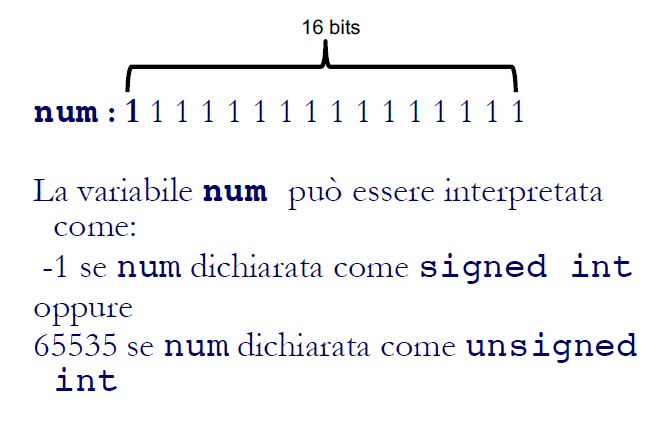
\includegraphics{C:/Users/giova/Documents/1_UNI/programmazione1/appunti/appunti-prog1/image/image-20201015171916756.png}
    \caption{image-20201015171916756}
    \end{figure}
  \end{itemize}
\item
  Da notare come tutti i valori massimi dei tipi di dati predefiniti è
  contenuto nella libreria \emph{limits.h}

\begin{lstlisting}[language=C]
#include <limits.h>
// racchiude i valori minimi e massimi della mia variabile
// dichiara il valore massimo e minimo del valore della variabile in una certa architettura
sizeof(nomevariabile); // restituisce il numero di byte
// es. char = 1, in generale restituisce il numero di byte assegnati a una variabile passata al costrutto.
// anche se il valore unsigned viene decrementato di uno, riceverò un valore positivo, nonstante fosse stato inizializzato a zero.
unsigned long int x;
printf("%d", x); // print valore intero della variabile e con il rispettivo sengno, anche se dichiarata unsigned. QUesto avviene perchè converte il valore da long a int.
\end{lstlisting}
\end{itemize}

Si noti anche la differenza fra float e double:

\begin{itemize}
\tightlist
\item
  float (6 cifre di precisione)
\item
  double (15 cifre di precisione)
\item
  Lo spazio di memoria sarà quindi (in ordine crescente): \emph{float
  \textless{} double \textless{} long double}
\end{itemize}

NOTA BENE CHE: è rischioso usare un \passthrough{\lstinline!if (a==b)!},
in cui \passthrough{\lstinline!a!} di tipo \emph{int} e
\passthrough{\lstinline!b!} di tipo \emph{float}, perché la condizione
potrebbe non risultare mai corretta, siccome generalmente il tipo
\emph{float} ha molta più precisione del tipo \emph{int} e anche che
l'uguaglianza per tornare vera, deve necessariamente avere tutte cifre
di \passthrough{\lstinline!a!} uguali a tutte le cifre di
\passthrough{\lstinline!b!}.

Inoltre il tipo di dato \emph{char} viene usato come un\emph{unsigned
int} e quindi ha senso a scrittura \passthrough{\lstinline!A!},
\passthrough{\lstinline!B!} in cui si usa il valore numerico del
carattere ASCII.

\hypertarget{conversioni-di-tipo}{%
\subsubsection{Conversioni di Tipo}\label{conversioni-di-tipo}}

Come si diceva precedentemente il tipo di dato consente di fare un
controllo sulla variabile, ma può anche avvenire di aver la necessità di
una conversione fra variabili, per cui si è citata l'operazione di
\emph{casting}. Questa operazione segue un meccanismo automatico, in
modo che io non debba preoccuparmi di quello che succede a basso livello
per la conversione, e permette una corretta conversione tra variabili
non uguali.

Il C fornisce un metodo per il \emph{casting} che però necessità di
attenzione al momento dell'utilizzo, per fare in modo che le variabili
non perdano valore. Generalmente il C lavora con le regole della
precedenza al momento dell'assegnazione, quindi viene convertito il
valore a sinistra dell'operatore di
assegnamento(\passthrough{\lstinline!=!}).

\emph{NOTA BENE:} le conversioni automatiche possono essere molto
particolari, quindi prestare molta attenzione al tipo di dato che
tornano.il problema è sempre la codifica di oggetti, come ad esempio int
o float (che si presuppone una perdita di cifre dopo la virgola), che
sono anche piuttosto simili, ma quando si inizia a dover comparare un
int con un char inizia a essere più complicato.

Per fare questo si seguono delle regole che il C segue e a cui noi
quindi ci atteniamo.

\begin{figure}
\centering
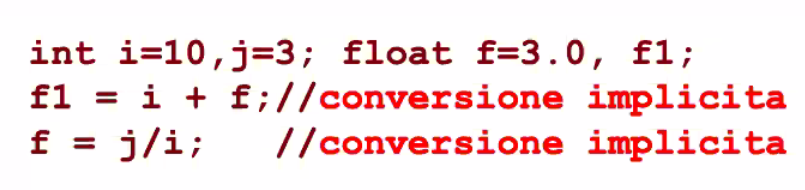
\includegraphics{C:/Users/giova/Documents/1_UNI/programmazione1/appunti/appunti-prog1/image/image-20201020113449566.png}
\caption{image-20201020113449566}
\end{figure}

Facendo una conversione implicita, il compilatore si occupa di
convertire le variabili in modo che siano dello stesso tipo.

\begin{figure}
\centering
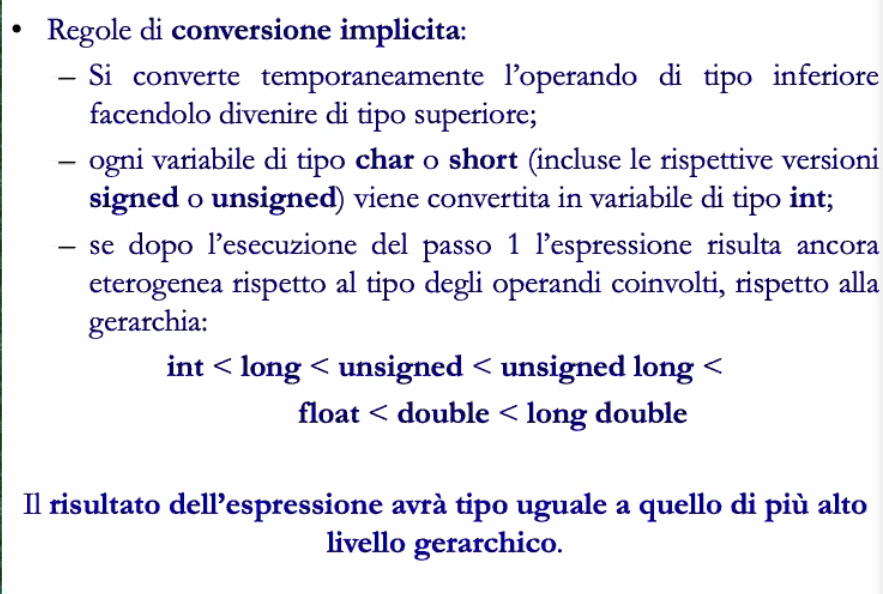
\includegraphics{C:/Users/giova/Documents/1_UNI/programmazione1/appunti/appunti-prog1/image/image-20201020113717182.png}
\caption{image-20201020113717182}
\end{figure}

Si eseguono tutte le azioni in ordine in modo che le variabili di tipo
inferiori diventino superiori, di conseguenza se devo fare:

\begin{lstlisting}[language=C]
int a == float b; 
    int a => float a;
    float a == float b;
\end{lstlisting}

Per rendere meglio comprensibile/visibile o per rendere il codice più
ordinato/leggibile, si usa la keyword \emph{(cast)}.

\begin{lstlisting}[language=C]
float media;
int num1=5, num2=3;
everage = (num1+num2)/2; // in questo caso ci affidiamo alla converione implicita, il valore mancherà di cifre decimali

// se invece 
everage = (float) (num1+num2)/2; // risultato corretto, ma anche più leggibile.
\end{lstlisting}

L'operatore di casting è uno di quelli che ha la precedenza su molto,
nell'ordine in cui si eseguono le operazioni (tabella di precedenza).

\emph{Ad Esempio:}

Per calcolare il valore di \[
\pi
\] con precisione a piacere usando l'approssimazione di Leibniz:

\begin{figure}
\centering
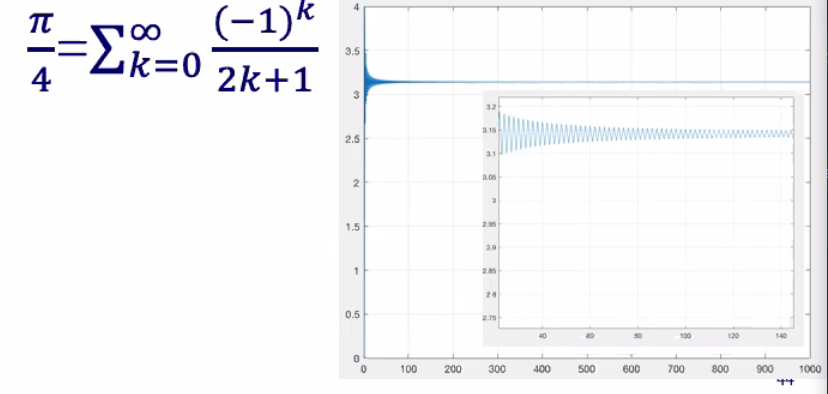
\includegraphics{C:/Users/giova/Documents/1_UNI/programmazione1/appunti/appunti-prog1/image/image-20201020115026359.png}
\caption{image-20201020115026359}
\end{figure}

Questo metodo (ma soprattutto dal grafico di questo metodo) si comprende
che è possibile calcolare il pigreco con un certo grado di precisione.
Per avere 4 cifre piuttosto convergenti bisogna, come si vede appunto
dal grafico, usare almeno un centino di cifre.

\emph{Implementazione del metodo di Liebnitz: (nel main)}

\begin{lstlisting}[language=C]
int i;
int precisione;
int segno = -1;
float pigreco = 1;

scanf("%d", &precisione);

for (i=1; i<=precisione; i++){
    pigreco += segno * 1/(2*i+1);
    
    printf("%f\n", pigreco*4);
    segno = (-1) * segno
}
\end{lstlisting}

In questo programma, in cui si usa la conversione implicita, che porta a
un errore di approssimazione, perché la conversione implicita nel caso
di divisone tra due variabili \textbf{int} causa un numero intero che
logicamente manca del resto dalla divisione stessa.

Con il casting in modo esplicito, il programma funziona meglio, e
soprattutto non lascia posto alla possibilità che il compilatore possa
ogni tanto fare correttamente e in altri casi sbagliando la conversione
implicita.

\hypertarget{tipi-user-defined-in-c}{%
\subsubsection{Tipi user-defined in C}\label{tipi-user-defined-in-c}}

Per usare variabili più complesse che siano definite puramente dal
programmatore e contengano al loro interno più variabili e di più tipi,
sia \emph{user-defined} sia predefinite si utilizza uno \emph{struct} ,
ovvero variabili strutturate.

Tutto ciò permette di creare variabili molto complesse, con una serie di
caratteristiche diverse fra di loro.

\begin{lstlisting}[language=C]
struct Impiegato{
    char Nome[20];
    char Cognome[20];
    float Stipendio;
    char CodiceFiscale[16];
}
\end{lstlisting}

Alla fine di questa definizione di struttura, che descrive come sarà
questa variabile, non viene allocata nessuna memoria, ma è solo un passo
formale del C.

Però com'è che si fa ad accedere a queste variabili? Ad esempio negli
array sapevo come erano i campi e l'unica cosa a cui dovevo stare
attento era di non sorpassare il numero di spazi assegnati nel
richiamare i caratteri. Se non più seguire una dichiarazione questa
funzione \emph{struct} non ha valore (vuol dire che la dichiaro e poi
posso iniziare a usarla).

\begin{lstlisting}[language=C]
struct Impiegato{
    char Nome[20];              // DEFINIZIONE
    char Cognome[20];           // DEFINIZIONE
    float Stipendio;            // DEFINIZIONE
    char CodiceFiscale[16];     // DEFINIZIONE
} amministratore, segretario;   //DICHIARAZIONE

struct Impiegato staff1,staff2; //DICHIARAZIONE 
//Da qui in poi posso iniziare a usarla, siccome la ho dichiarata
\end{lstlisting}

All'interno dello \emph{struct} non importa l'ordine (a meno che una
variabile dipenda da un altra, in questo caso la variabile indipendente
va dichiarata prima). infatti al compilatore non cambia se metti prima
il nome o il cognome, perché poi la variabile viene richiamata in ugual
modo. (Nessun cambio di ordine della definizione porta a miglioramento
delle prestazioni, il programma ci mette ugual tempo a definire prima un
campo di un altro).

Per indicizzare i campi all'interno dello \emph{struct} viene usata la
\emph{dot notation}:

\begin{lstlisting}[language=C]
impiegato.Stipendio = 0.0;      // assegno al campo stipendio dello struct impiegato uguale a zero
// dopo aver inizializzato queste cose, poi posso stilare l'albero sintattico per usare lo struct come variabile normale:

if (impiegato.Stipendio < 2000){
    impiegato.Stipendio = 1.5 * impiegato.Stipendio;
}
\end{lstlisting}

Il \emph{dot operator} è in cima alla tabella delle precedenze di
traduzione, in linea con l'ordine di precedenza delle parentesi.

Il construtto \emph{struct} occupa in memoria esattamente la somma della
memoria occupata dagli elementi che lo compongono.

\hypertarget{strutture-complesse}{%
\subsubsection{Strutture complesse}\label{strutture-complesse}}

Le strutture complesse sono variabili strutturate che usano a loro volta
variabili strutturate al loro interno. Ad esempio:

\begin{lstlisting}[language=C]
struct lato{
    int lunghezza;
    int x;
    int y;
}
struct rettangolo{
    lato lato-lungo;
    lato lato-corto;
}
\end{lstlisting}

Se all'interno dello \emph{struct} è dichiarato un campo che a sua volta
è uno \emph{struct}, allora il dot operator sarà riutilizzato fino ad
ottenere il campo ricercato.

\begin{lstlisting}[language=C]
struct Data{                // definizione Data
    int giorno;
    int mese;
    int anno;
};

struct Data mia-data;       // dichiarazione Data

struct Agenda{              // definizione Agenda
    char[10] NomeEvento;
    mia-data DataEvento;
}

struct Agenda mia-agenda;   // dichiarazione Agenda

mia-agenda.mia-data.mese = 12;
                            // accedo al campo di Agenda, che è sua volta una variabile strutturata.
\end{lstlisting}

\hypertarget{utilizzo-del-typedef}{%
\subsubsection{\texorpdfstring{Utilizzo del
\emph{typedef}:}{Utilizzo del typedef:}}\label{utilizzo-del-typedef}}

L'idea è quello di creare un meccanismo sintattico formale in modo che
io possa usare degli altri nomi per definire e chiamare le variabili,
che possono essere variabili semplici o strutturate.

Di solito il \emph{typedef} è posto tra la definizione di costanti e il
main().

Il \emph{typedef} funziona creando una tabella di sinonimi che
rappresentano in realtà tipi di dati predefiniti o user-defined, ma che
hanno il lato positivo di comparire al programmatore con un nuovo nome,
appunto un sinonimo. Il nuovo tipo eredita le operazioni del tipo di
partenza e ne è uguale, eccetto per il nome a cui ci si riferisce per
richiamarlo. Ad esempio:

\begin{lstlisting}[language=C]
typedef int intero;  //definisco alias per 'int' chiamato intero
intero numero;       // difinisco un tipo 'intero' esattamente come fosse un qualsiasi altro tipo
\end{lstlisting}

Il \emph{typedef} non si basa sulla ereditarietà, cioè non funziona che
gli elementi prendono il valore di quelli di partenza perché lo
``ereditano'', ma proprio perché il compilatore crea una tabella di
sinonimi che viene usata al momento della compilazione per sostituire
direttamente il tipo di dato originale al posto del suo alias presente
nel codice.

Dove si usa:

\begin{itemize}
\tightlist
\item
  nel caso di variabili che ricorrono spesso e necessitano di essere più
  comprensibili/utilizzabili.
\item
  evitare di definire più volte lo stesso tipo di variabile
\end{itemize}

\begin{lstlisting}[language=C]
typedef char[10] NomePersona;
typedef NomePersona CognomePersona;
// adesso il tipo NomePersona è uguale al tipo CognomePersona che a sua volta è uguale a dire char[10]. Ma allo stesso modo posso anche dichiarare:
NomePersona Persona1, Persona2, Persona3;
\end{lstlisting}

A questo punto il programmare diventa sempre più a pensare a che cosa
scegliere, in modo che il programma sia il più comprensibile e
utilizzabile possibile.

\begin{lstlisting}[language=C]
typedef int Vettore[20];
typedef Vettore Vettore20per20;
typedef vettore Nome;
// osso dichiarare una serie di cose usando sempre il tipo vettore

// a questo punto posso io a priori dichiare delle costanti a un tipo di dato in modo che mi venga più comodo il suo uso.
\end{lstlisting}

\hypertarget{utilizzo-del-enum}{%
\subsubsection{\texorpdfstring{Utilizzo del
\emph{enum}:}{Utilizzo del enum:}}\label{utilizzo-del-enum}}

Un sottotipo di variabile \emph{struct} è l'\emph{enum} per indicare una
variabile strutturata che può prendere solo un valore finito e
predeterminato di valori.

Questo tipo di variabile è molto utile ad esempio se si vuole usare una
lista di cose di cui si conosce tutto, e che deve essere presa come
variabile comprensibile al compilatore all'interno del programma. Un
altra caratteristica è che all'interno della variabile \emph{enum} il
compilatore assegna a ogni valore, un'alias di valore \emph{int}.

Ad esempio un \emph{enum} potrebbero essere i giorni della settimana a
cui ad ogni giorni si associa un valore \emph{int}, in modo da poter
fare facilmente cicli con i numeri.

\begin{lstlisting}[language=C]
enum Settimana {
    lun, mar, merc, giove, sab, dom
        // lun = 0; mar = 1; merc = 2, giove = 3; ...
}
\end{lstlisting}

\hypertarget{puntatori}{%
\subsection{Puntatori}\label{puntatori}}

I puntatori sono un elemento necessario per la programmazione in C per:

\begin{itemize}
\item
  costruzione di funzioni
\item
  allocazione dinamica
\item
  efficienza dei programmi in memoria
\end{itemize}

I puntatori hanno il lato positivo nel fatto che permettono un
grandissimo uso della memoria e quindi aiutano a rendere il programma
più efficiente, al contrario però il loro utilizzo potrebbe causare
errori di allocamento di memoria o di sovrascrittura di un luogo di
memoria. Di conseguenza i puntatori sono un punto di forza del C, ma
anche punto di debolezza.

il concetto di puntatore si deve vedere come una variabile che contiene
essa stessa l'indirizzo di memoria. Adesso la variabile puntatore
contiene invece solo l'indirizzo, lasciando quindi libero lo spazio
necessario all'allocazione di un valore.

Questo concetto è molto diverso da quello di una normale variabile,
nella quale era contenuto sia il tipo di dato sia il suo indirizzo di
memoria.

ATTENZIONE CHE: il puntatore non da garanzie che all'interno di quello
spazio di memoria ci sia qualcosa o se quello che è presente sia
comprensibile.

La rappresentazione più efficace del puntatore è come quella che segue:
il quadrato rappresenta il puntatore, la freccia invece indica a cosa
punta il valore. Sopra il quadrato è presente l'identificatore del
puntatore. La freccia arriva in una zona con un solo tipo di dato e poi
identificata da un nome.

\begin{figure}
\centering
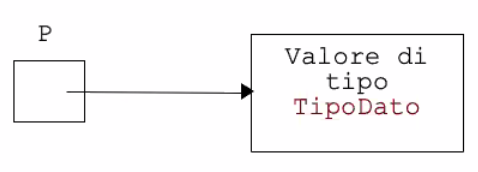
\includegraphics{C:/Users/giova/Documents/1_UNI/programmazione1/appunti/appunti-prog1/image/image-20201022154400716.png}
\caption{image-20201022154400716}
\end{figure}

\begin{lstlisting}[language=C]
// sintassi per la dichiarazione di un puntatore:
TipoDato *Puntatore;
\end{lstlisting}

Il tipo di dato che viene assegnato al puntatore è necessario affinché
il compilatore del C riesca a tradurre quello che viene indicato dalla
variabile stessa. Di fatto, il puntatore non ha un tipo predefinito.

Un puntatore è definibile anche attraverso un \emph{typedef}:

\begin{lstlisting}[language=C]
typedef TipoDiDato *TipoDiDatoPuntato;
\end{lstlisting}

\hypertarget{operatore-e-dereferenziazione-e-indirizzo-di}{%
\subsubsection{\texorpdfstring{Operatore \texttt{*} e \texttt{\&}
(dereferenziazione e indirizzo
di)}{Operatore * e \& (dereferenziazione e indirizzo di)}}\label{operatore-e-dereferenziazione-e-indirizzo-di}}

Questi operatori servono per operare con i puntatori e con gli indirizzi
di memoria.

L'operatore di \textbf{dereferenziazione} ha principalmente due
funzioni:

\begin{itemize}
\tightlist
\item
  nella dichiarazione del puntatore, indica che la variabile dichiarata
  \emph{è} un puntatore
\item
  in qualsiasi altro uso, per recuperare il valore della variabile,
  ovvero il contenuto dello spazio a cui sta puntando.
\end{itemize}

Utilizzo generale:

\begin{lstlisting}[language=C]
// nella dichiarazione, indica che si sta indicando un puntatore
TipoDiDato *PuntatoreTipoDiDato;

// Presa la variabile 'IndirizzoAlTipoDiDato' come un indirizzo
PuntatoreTipoDiDato = IndirizzoAlTipoDiDato; 

// viene assegnato un TipoDiDato, al valore del punatore
*PuntatoreTipoDiDato = ValoreTipoDiDato; 

// Per accedere al valore del puntatore si deve usare ancora deferenziare:
printf(*PuntatoreTipoDiDato); // Stampa: ValoreTipoDiDato
\end{lstlisting}

Da come si vede nell'esempio è importante specificare il tipo di dato
del puntatore, perché l'operatore di dereferenziazione non fornisce
queste informazioni. Se non si specifica il tipo di dato non si stanno
fornendo al compilatore informazioni necessarie per \emph{tradurre} il
contenuto del suo valore.

L'operatore \textbf{indirizzo di} al contrario permette di calcolare un
indirizzo di memoria di una data variabile.

\begin{lstlisting}[language=C]
Puntatore *P;
P = &x;
// L'operatore '&' fa in modo da restituire l'indirizzo della variabile x, che poi viene assegnato al puntatore P
\end{lstlisting}

Questo metodo è molto conveniente per evitare di dover inserire
manualmente il valore dell'indirizzo di memoria di una certa variabile.
Questo modo è molto comodo anche per cambiare il right-value al
puntatore.

Esempio:

\begin{lstlisting}[language=C]
// Dichiaro Puntatori P, Q e inizializzo a NULL, e un TipoDato y
Tipopuntatore P, Q;
TipoDato y = 10;
P = NULL;
Q = NULL;

printf("%d ", y);

// Inizializzo il puntatore sull'indirizzo di y
P = &y; 

// Cambio il valore della variabile puntata
*P = 14;

printf("%d", y); //14
printf("%d", *P);// 14

y++;

printf("%d", y); //15

Q = P; 
// Sto dicendo che all'indirizzo di memoria che era indicato in P adesso punta anche Q. Adesso ci sono 3 modi per accedere/modificare quella variabile.

printf("%d", *Q); // 15
\end{lstlisting}

Entrambi gli operatori \passthrough{\lstinline!*!} e
\passthrough{\lstinline!\&!} sono inseriti al secondo posto nella
tabella delle precedenze, superati delle parentesi e dagli operatori
\passthrough{\lstinline!.!} e \passthrough{\lstinline!->!}.

\hypertarget{problematiche-e-rischi-con-i-puntatori}{%
\subsubsection{Problematiche e Rischi con i
puntatori:}\label{problematiche-e-rischi-con-i-puntatori}}

L'utilizzo dei puntatori è facile ma anche potenzialmente pericoloso,
principalmente stare attenti che:

\begin{itemize}
\tightlist
\item
  esiste il problema dell'accesso multiplo (più puntatori allo stesso
  luogo di memoria), questo problema è detto \textbf{aliasing}
\item
  il codice perde leggibilità e immediatezza nella comprensione quasi
  immediatamente, quindi diventa più difficoltoso ottenere un codice
  pulito e ordinato.
\item
  non vengano persi valori, eliminando un puntatore, come si vede sotto.
  Il valore di y infatti non è più recuperabile dopo questa operazione,
  e occuperà sempre un valore di memoria inutilizzabile dal resto del
  programma.
\end{itemize}

\begin{figure}
\centering
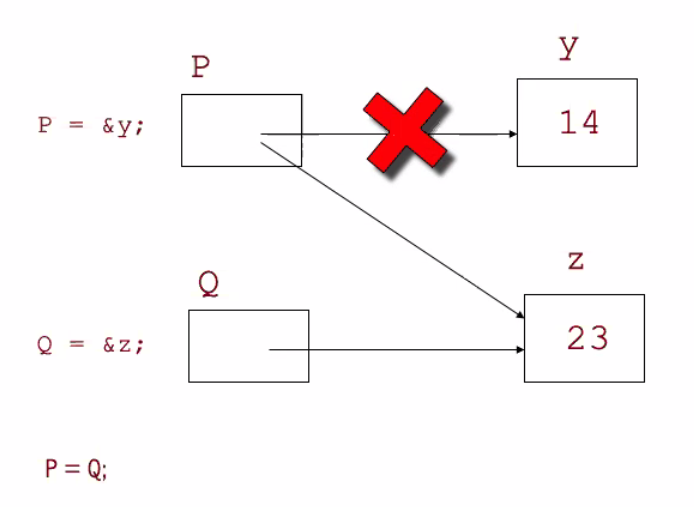
\includegraphics{C:/Users/giova/Documents/1_UNI/programmazione1/appunti/appunti-prog1/image/image-20201022170000134.png}
\caption{image-20201022170000134}
\end{figure}

\hypertarget{puntatori-dot-notation-e-variabili-strutturate}{%
\subsubsection{Puntatori, Dot-notation e Variabili
Strutturate:}\label{puntatori-dot-notation-e-variabili-strutturate}}

Esempio di Struct con l'uso di puntatori:

\begin{lstlisting}[language=C]
// dichiaro uno struct
typedef struct {
    int PrimoCampo;
    char SecondoCampo;
}TipoDato;

// nel MAIN, dichiaro x e *P come TipoDato, e assegno al puntatore l'indirizzo di x
TipoDato x, *P;
P = &x;

// Per accedere alle classi della variabile strutturata, rispettando le precedenze degli operatori:

(*P).PrimoCampo = 12; // Anche se le parentesi tonde non sono necessarie

*P.PrimoCampo = 12;   // Perchè la Dot-notation ha massima priorità

// Esiste anche una sintassi abbreviata per il puntatore a una struttura:
P -> PrimoCampo = 12; // questo operatore si trova in cima priorità
\end{lstlisting}

Da ricordare poi l'operatore unario \textbf{sizeof()} che restiuisce il
numero di byte di una variabile.

\hypertarget{i-tipi-di-dato-con-i-puntatori}{%
\subsubsection{I tipi di dato con i
puntatori:}\label{i-tipi-di-dato-con-i-puntatori}}

il puntatore come detto è una variabile che non ha un tipo predefinito,
ma gliene viene assegnato uno al momento della dichiarazione, azione
necessaria affinché il compilatore capisca quello che contiene il valore
del puntatore stesso.

Per questo motivo, i puntatori possono essere utilizzati anche con le
altre keyword che definiscono le variabili, in particolare si fa notare
\textbf{const}.

La keyword \emph{const} può diventare necessaria nel caso in cui le
variabili debbano essere accessibili in sola lettura, quindi evitare che
vengano modificate.

La keyword \emph{const} non va scambiato con \emph{define}:

\begin{itemize}
\tightlist
\item
  \emph{define} è un operazione che avviene a livello del linker,
  operando semplicemente una sostituzione attraverso tabella di
  sinonimi.
\item
  \emph{const} crea una tabella dei sinonimi indicando che la data
  variabile non si può modificare
\end{itemize}

Esistono due modi per protegger il puntatore, nel primo proteggiamo il
puntatore, nonostante la variabile puntata possa ancora cambiare:

\begin{lstlisting}[language=C]
int * const ptr = &x; 
\end{lstlisting}

Se invece voglio un puntatore che contenga una variabile non
modificabile devo usare un doppio \emph{const}:

\begin{lstlisting}[language=C]
const int * const ptr = &x;
\end{lstlisting}

\hypertarget{aritmetica-dei-puntatori}{%
\subsubsection{Aritmetica dei
puntatori:}\label{aritmetica-dei-puntatori}}

L'aritmetica dei puntatori è necessaria per sommare indirizzi, o
modificare il valore puntato dell'indirizzo.

Operatori di autoincremento con i puntatori o di modifica della
variabile puntata:

\begin{lstlisting}[language=C]
// Dichiaro e assegno il puntatore
int x=1;
int *ip;
ip = &x;

// vado ad incrementare di 10 il valore che trovo dentro il banco di memoria
*ip = *ip+10;
// Valore x: 11

// incrementa la variabile puntata da *ip di uno
*ip += 1; 
// Valore x: 12

++*ip; 
(*ip)++;
// In questo caso i due operatori hanno lo stesso risultato, ma:
// NB: gli operatori * e di autoincremento(++x, x++) hanno stessa precedenza, di conseguenza il compilatore avrebbe associato da destra e il risultato potrebbe risultare diverso.
\end{lstlisting}

Aritmetica degli indirizzi:

\begin{lstlisting}[language=C]
int y[] = {1, 2, 3, 4, 5};
int *p = &y; // puntatore inizializzato a y[0]

*(p+1) == 2; // Al puntatore viene aggiunto l'indizzo dello spazio di un intero, siccome il puntatore è inizializzato ad intero. Questo significa praticamente che si prende il valore intero +1 rispetto al puntatore.
*(1+p) == *(p+1); 
\end{lstlisting}

Per questo motivo si può dedurre che:

\begin{lstlisting}[language=C]
// Dichiaro un array di numeri (un vettore), e poi assegno al puntatore a intero l'indirizzo del primo elemento del vettore. 
int a[10];
int *p;

a[i] == *(a+i); 
// *(a+i) è l'indirizzo di 'a' più 'i', quindi ne risulta l'elemento appartenente all'insieme 'a' in posizione 'i'
// 'i' in realtà non incrementa propriamente di i, ma di i*sizeof(TipoPuntatore)

// Questo vuol dire che: inizializzare p al primo elemento del vettore in questi due modi è equivalente
(p = &a) == (p = &a[0]);
(p = &(a+1)) == (p = &a[1]);

// Al contrario NON sono ammessi: (perchè sto sbagliando l'assegnamento a destra)
a = p;
a = p+1;

// Sottrazione con puntatori:
int *q;

p-q; // Restituisce il numero di elementi di differenza tra i due puntatori, ovvero il numero di spazi di memoria tra i due. ATTENZIONE: NON RESTITUISCE LA DIFFERENZA FRA I VALORI DEI DUE PUNTATORI
\end{lstlisting}

Si possono anche costruire array di puntatori:

\begin{lstlisting}[language=C]
const char *semi[4] = {
    "Cuori",
    "Picche",
    "Fiori",
}
\end{lstlisting}

Questo è un array fatto con valori di stringhe costanti. Si può anche
fare con valori di stringhe variabili, attraverso un array di puntatori
non costanti.

\hypertarget{relazione-tra-array-e-puntatori-in-c}{%
\subsubsection{Relazione tra Array e Puntatori in
C}\label{relazione-tra-array-e-puntatori-in-c}}

Se si provasse a scrivere un programma che usasse una variabile a
puntatore come array di caratteri cosa succederebbe?

\begin{lstlisting}[language=C]
int main (){
    
    char stringa[] = "Ciao Mondo";
    char *stringaP = "Ciao Terra";
    
    printf("Stringa = %s \n", stringa);
    printf("StringaP = %s \n", stringaP);
    
}
\end{lstlisting}

Questo funziona perché l'operatore \passthrough{\lstinline![]!} nel C
viene usato come il puntatore al primo elemento dell'array, quindi se ne
deduce anche che, per l'aritmetica dei puntatori:

\begin{lstlisting}[language=C]
char *stringa == char stringa[];

stringa[5] == *(stringa+5);

stringa[5] == *(5+stringa);

stringa[5] == 5[stringa];
\end{lstlisting}

Attenzione alla modifica del puntatore a stringa, perché modificandolo
si può perdere l'inizio della stringa, facendo l'errore dell'aliasing
(sopra).

Quindi per scorrere i valori di una stringa implementata con un
puntatore abbiamo bisogno di un puntatore di servizio:

\begin{lstlisting}[language=C]
char *stringa = "Il sale della vita";
char *p;
int len = 0;
// variabile ptr p, con il valore di stringa, presa a variabile intermedia.
p = stringa;

while (*p++ != '\0')
    ++len;
printf("Lunghezza stringa %s: %d\n", stringa, len)
\end{lstlisting}

\hypertarget{le-funzioni-in-c}{%
\subsection{Le funzioni in C}\label{le-funzioni-in-c}}

Le funzioni nel C hanno diverse motivazioni:

\begin{itemize}
\tightlist
\item
  evitare di riscrivere intere operazioni \textbf{ripetute}, con il
  rischio di introdurre errori.
\item
  scrivere blocchi \textbf{riutilizzabili}, da programmi/programmatori
  differenti.
\item
  \textbf{incapsulamento} di algoritmi e possibilità di creare un
  \textbf{interfaccia} tra i programmi (ovvero differenza tra compito da
  eseguire e come questo venga eseguito).
\item
  si possono scrivere \textbf{librerie}, ovvero insiemi di funzioni per
  eseguire determinate azioni definite
\end{itemize}

Le funzioni nel C:

\begin{itemize}
\tightlist
\item
  hanno bisogno di risorse per essere eseguiti
\item
  devono avere tutti gli elementi di sintassi formale necessari affinché
  la funzione effettivamente funzioni e restituisca un valore corretto.
\item
  si scorpora il codice in un \textbf{programma chiamante} e un
  \textbf{programma chiamato}.
\end{itemize}

\hypertarget{funzionamento-della-macchina-astratta-del-c-e-lasservimento-delle-funzioni}{%
\subsubsection{Funzionamento della macchina astratta del C e
l'asservimento delle
funzioni}\label{funzionamento-della-macchina-astratta-del-c-e-lasservimento-delle-funzioni}}

I \textbf{sottoprogrammi} sono asserviti a sottoprogrammi chiamanti.
Affinché questo sottoprogramma funzioni, c'è bisogno che all'interno del
programma chiamato siano presenti tutti i parametri necessari a
funzionare, sia che questi debbano essere passati da un altro
sottoprogramma, sia che debbano solo essere accessibili.

Esistono due tipi di sottoprogrammi:

\begin{itemize}
\item
  \emph{funzioni}, che restituiscono un valore al chiamante.
\item
  \emph{procedure}, che svolgono un compito per il chiamante, ma non
  restituiscono nessun valore (definiti con \emph{void}, che è la
  keyword che indica nessun valore o tipo e serve per rispettare la
  sintassi formale della dichiarazione delle funzioni).
\end{itemize}

\hypertarget{struttura-di-un-programma-c}{%
\subsubsection{Struttura di un programma
C}\label{struttura-di-un-programma-c}}

In un programma solitamente, è presente:

\begin{itemize}
\item
  il sottoprogramma \emph{main}, ovvero il principale, tutti quello che
  è preceduto da \passthrough{\lstinline!\#!} è un indicazione al
  linker.

\begin{lstlisting}[language=C]
#include <libreria>
#include "programma.h"

#define MACRO valoreMAcro

int main() {
  // codice
}
\end{lstlisting}

  \begin{itemize}
  \tightlist
  \item
    \passthrough{\lstinline!\#include <libreria>!} serve per aggiungere
    delle librerie standard
  \item
    \passthrough{\lstinline!\#include "programma.h"!} serve per
    aggiungere librerie presenti nella stessa cartella del file che
    contiene il \emph{main}.
  \item
    \passthrough{\lstinline!\#define MACRO valoreMacro!} crea un alias
    che sostituisce il valore della macro al nome della macro.
  \end{itemize}
\item
  Una serie di sottoprogrammi che si possono chiamare
\item
\begin{lstlisting}[language=C]
  int funzione(int valore1, int valore2){ // questa linea è chiamata testata
    // codice
  }
\end{lstlisting}

  \begin{itemize}
  \tightlist
  \item
    \passthrough{\lstinline!int!} all'inizio è il \emph{parametro di
    ritorno della funzione}. Può essere un tipo di variabile predefinito
    o uno user-defined
  \item
    \passthrough{\lstinline!funzione!} è il \emph{nome della funzione}
  \item
    \passthrough{\lstinline!(int valore1, int valore2)!} sono i
    \emph{parametri o valori formali}. Indicano i parametri che vanno
    forniti alla funzione e il tipo di questo parametro. C'è la
    possibilità di aver tipo di parametri sia predefiniti che
    strutturati.
  \item
    \passthrough{\lstinline!\{ //codice \}!} è il luogo dove il
    programma si svolge quando la funzione viene chiamata, ovvero il
    \emph{corpo della funzione}. Questa può contenere una \emph{parte
    dichiarativa locale}, dove vengono definite le variabili necessarie
    all'esecuzione, e una \emph{parte programmatica} che contiene
    l'algoritmo del programma.
  \end{itemize}
\end{itemize}

Nel C i sottoprogrammi hanno:

\begin{itemize}
\tightlist
\item
  la \emph{definizione} del programma, che comprende sia la testata che
  il corpo della funzione
\item
  la \emph{dichiarazione} della funzione, chiamata anche
  \emph{prototipo}, che comprende solo la testata.
\end{itemize}

\begin{lstlisting}[language=C]
int funzione(int valore1, int valore2); // questa è una dichiarazione o prototipo

int funzione(int valore1, int valore2){ // questa una definizione del programma
    // codice
}
\end{lstlisting}

\hypertarget{collegamento-tra-funzione-e-chiamante}{%
\paragraph{Collegamento tra funzione e
chiamante}\label{collegamento-tra-funzione-e-chiamante}}

Al momento della restituzione del valore al programma chiamante possono
succedere due cose. O il programma ha un ritorno di tipo \emph{void}
quindi non ritorna nulla, oppure ha un tipo di variabile che deve
restituire. In questo caso, allora:

\begin{itemize}
\item
  la funzione non restituisce nessun valore, quindi la funzione termina
  con l'ultima istruzione prima delle parentesi graffe
\item
  la funzione termina con \passthrough{\lstinline!return;!}
\item
  la funzione termina con \passthrough{\lstinline!return espressione;!},
  allora il valore dell'\emph{espressione} viene passato al programma
  chiamante. L'\emph{espressione} può essere:

  \begin{itemize}
  \tightlist
  \item
    tipo di dato predefinito o user-defined, che coincide con il
    \emph{parametro di ritorno}
  \item
    \textbf{non} può restituire un array
  \item
    \textbf{può} restituire puntatori, così rende possibile passare
    strutture molto grandi molto velocemente
  \item
    può essere restituito solo un valore
  \end{itemize}
\end{itemize}

Nel sottoprogramma si possono avere delle variabili locali, che vengono
dichiarate normalmente e che servono per l'effettivo svolgimento del
programma. Il loro valore può essere restituito anche con il
\passthrough{\lstinline!return valore;!}.

\hypertarget{parametri-formali-e-effettivi}{%
\paragraph{Parametri formali e
effettivi}\label{parametri-formali-e-effettivi}}

Ci sono due tipi di parametri:

\begin{itemize}
\tightlist
\item
  parametri \emph{formali} sono quelli elencati nella testata
\item
  parametri \emph{effettivi} sono quelli con la quale la funzione viene
  invocata
\end{itemize}

I parametri formali vengono inizializzati con valori dei parametri
effettivi. Di fatto il programma chiamante si occupa di creare i
parametri effettivi per chiamare la funzione attraverso i parametri
formali della funzione. Al momento in cui questi parametri vengono
passati, l'ordine conta. Questo vuol dire che i parametri effettivi
devono essere i corrispettivi dei parametri formali dichiarati nel
sottoprogramma. Questo vuol dire anche che prima di usare una funzione,
è necessario che questa sia \emph{definita}, ovvero che siano stati
dichiarati la testata e il codice della funzione.

\hypertarget{modello-di-esecuzione-e-il-concetto-di-ambiente}{%
\subsection{Modello di esecuzione e il concetto di
ambiente}\label{modello-di-esecuzione-e-il-concetto-di-ambiente}}

Prendiamo un esempio di programma che utilizza funzioni chiamanti e
sottoprogrammi:

\begin{lstlisting}[language=C]
int x = 0;
int f1(int p);
void f2();

main(){
    f2();
}
int f1(int p){
    return p+x;
}
void f2(){
    printf("%d", f1(x));
}
\end{lstlisting}

Ogni sottoprogramma crea in memoria uno spazio, chiamato
\emph{ambiente}, che contiene le variabili locali, i parametri passati e
il risultato. Questo spazio di memoria viene rilasciato alla fine
dell'esecuzione del programma.

Posso pensare come se avessi una macchina dedicata che viene creata a
ogni esecuzione di quella funzione. Questa macchina viene allocata e
messa a disposizione quando la funzione viene istanziata, e poi viene
rilasciato deallocando tutta la memoria occupata quando ho finito il suo
utilizzo.

In realtà una sola macchina virtuale può eseguire questo comportamento.
L'immagine sotto è un ottima rappresentazione di quello che accade.

\begin{figure}
\centering
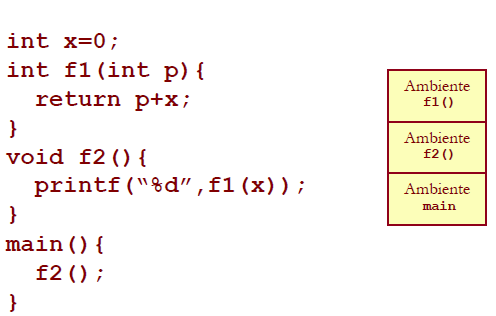
\includegraphics{C:/Users/giova/Documents/1_UNI/programmazione1/appunti/appunti-prog1/image/image-20201029162606113.png}
\caption{image-20201029162606113}
\end{figure}

Quando allocco memoria per un programma io di fatto sto costruisco una
pila, in cui i pezzi sono in contatto tra di loro e contengono i vari
ambienti delle funzioni, che a loro volta contengono le variabili
necessarie al funzionamento della funzione stessa. Questa struttura può
essere rappresentata dallo \textbf{stack}, chiamato anche pila, che fa
riferimento alla struttura LIFO (Last In First Out), una delle strutture
complesse viste più avanti.

Quando ho finito l'esecuzione di un ambiente posso rilasciarlo. Siccome
gli ambienti si sono accumulati dal basso verso l'alto, logicamente
rilasciando un ambiente alla volta, si smonterà lo stack dall'alto verso
il basso.

Quando una funzione viene invocata si crea una copia delle variabili che
vengono passate dalla funzione chiamante, mentre si deve ritornare il
risultato dell'ambiente prima che venga deallocato e quindi perdere
tutte le variabili non sono state passate. La copia delle variabili
permette di avere tutte le informazioni necessarie al funzionamento
della funzione corrente. Questo è utile e necessario, perché come
abbiamo visto, al momento della creazione di una funzione, si crea
l'ambiente necessario a quella funzione, che per forza di cose è diverso
dall'ambiente del programma chiamante. Passando il valore per copia,
quindi, ci si assicura che tutte le variabili necessarie al corretto
funzionamento siano presenti nell'ambiente corrente.

Lo svantaggio di questo metodo è la lentezza nello scrivere grosse
strutture di dati, un ingombro di memoria esagerato, soprattutto se la
variabile da copiare è molto grande, o è ad esempio un intero database,
che non si può replicare tante volte se no la memoria finirebbe.

Per ovviare a questo problema si usano i puntatori. Il puntatore infatti
è un oggetto molto piccolo che include al suo interno un indirizzo di
memoria, rendendolo così accessibile alla funzione. In questo modo di
fatto si sta modificando la variabile presente in un altro ambiente,
senza bisogno di avere una copia all'interno dell'ambiente corrente.
Questo però ha anche dei problemi, infatti in questo caso i cambiamenti
sulle variabili sono permanenti, e non si sta passando nessun valore
alla funzione chiamante per eseguire questi cambiamenti.

Il rischio nell'utilizzo dei puntatori è che nel caso di un errore nella
gestione del puntatore si possono creare gravi problemi di accesso a
sezioni di memoria non normalmente accessibili e c'è il rischio di
corrompere sezioni di memoria. Per cercare di risolvere in parte questo
problema si deve cercare di indicare i valori costanti nei puntatori.

Un esempio:

\begin{figure}
\centering
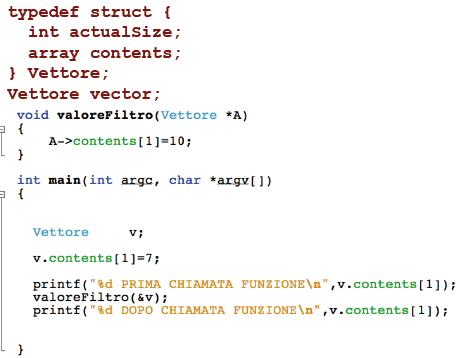
\includegraphics{C:/Users/giova/Documents/1_UNI/programmazione1/appunti/appunti-prog1/image/image-20201029170916817.png}
\caption{image-20201029170916817}
\end{figure}

In questa implementazione:

\begin{itemize}
\item
  Non ho copiato tutto il vettore V, ma solo il suo indirizzo e quindi
  siamo riusciti a diminuire lo spazio in memoria necessario
  all'esecuzione del programma.
\item
  Con questo uso siamo riusciti a modificare un valore appartenente al
  \emph{main}.
\item
  \passthrough{\lstinline!\&v!} al momento del passaggio del vettore
  serve perché è richiesto un puntatore nella definizione della
  funzione, e questo operatore restituisce l'indirizzo della variabile.
\end{itemize}

Il vantaggio di usare i puntatori in C consente nel fatto che si può
passare qualsiasi tipo di dato. Infatti usando uno \emph{struct} posso
gestire tutti i parametri formali e passo un'intera struttura con un
solo puntatore.

\hypertarget{passaggio-di-parametri-pro-e-contro}{%
\subsubsection{Passaggio di parametri pro e
contro}\label{passaggio-di-parametri-pro-e-contro}}

Il passaggio per \emph{valore} in una funzione:

\begin{itemize}
\tightlist
\item
  esegue una copia inefficiente se il parametro è ingombrante
\item
  parametro effettivo e formale occupano zone distinte di memoria
\item
  fornisce valori di ingresso
\end{itemize}

Il passaggio per \emph{indirizzo} in una funzione:

\begin{itemize}
\tightlist
\item
  permette la copia di un indirizzo di una variabile semplice o
  strutturata
\item
  la modifica avviene direttamente sul parametro effettivo
\item
  sono possibili effetti collaterali
\end{itemize}

\hypertarget{ambiti-di-visibilituxe0}{%
\subsubsection{Ambiti di visibilità}\label{ambiti-di-visibilituxe0}}

Per comprendere il concetto di visibilità delle variabili, si deve prima
comprendere quello di \emph{blocco}. Il blocco di codice nel C si
dichiara con \passthrough{\lstinline!\{ \}!} e può comparire in ogni
sintassi che consente un istruzione (nel corpo di una funzione, o in un
qualsiasi ciclo).

Due blocchi fra loro possono essere:

\begin{itemize}
\tightlist
\item
  \emph{annidati}, cioè l'uno dentro l'altro
\item
  \emph{paralleli}, cioè entrambi all'interno di un terzo blocco.
\end{itemize}

Per essere utilizzate le variabili devo essere visibili, ovvero il
programma deve sapere a cosa corrisponde l'identificatore della
variabile.

Se la dichiarazione avviene nella \textbf{parte dichiarativa locale}
allora le variabili sono visibili ovunque all'interno del suo blocco e i
blocchi che sono contenuti al suo interno.

Se la dichiarazione avviene nella \textbf{parte dichiarativa globale},
quindi esterno a qualsiasi blocco, la variabile è visibile da tutte le
funzioni, incluso \emph{main} e procedure e in tutti i blocchi del
programma.

Può avere \emph{side effect o effetti collaterali}, ovvero l'esecuzione
di una funzione non è più confinato all'interno del suo ambiente e
interessa variabili di altre funzioni, oppure tutto è accessibile, anche
quando non lo dovrebbe essere. Per questo motivo l'uso di variabili
globali è solitamente sconsigliato (da non confondere con le macro per
il linker, che invece possono essere molto utili).

Da ricordare il \emph{mascheramento}: se due variabili una globale e una
locale hanno lo stesso nome, il linker assegna il valore di quella
locale, di fatto mascherando eventuali omonimi.

\hypertarget{ciclo-di-vita-delle-variabili}{%
\paragraph{Ciclo di vita delle
variabili}\label{ciclo-di-vita-delle-variabili}}

Il normale ciclo di vita di una variabile va dal momento della
creazione/allocamento della memoria, fino alla distruzione/deallocamento
della memoria.

Esistono due classi di variabili:

\begin{itemize}
\tightlist
\item
  \textbf{statiche}:

  \begin{itemize}
  \tightlist
  \item
    allocate una volta e poi distrutte al termine dell'esecuzione del
    programma
  \item
    lo sono le variabili \emph{globali}
  \item
    persistenti all'interno e all'esterno di invocazioni di funzioni
  \item
    si può dichiarare una variabile o un blocco \emph{static} al momento
    dell'allocamento, che diventano persistenti all'interno ed
    all'esterno di invocazioni di funzioni.
  \end{itemize}
\item
  \textbf{dinamiche/automatiche}:

  \begin{itemize}
  \tightlist
  \item
    possono essere create e distrutte
    \emph{automaticamente}/implicitamente o esplicitamente dal
    programmatore con appositi construtti.
  \item
    sono dichiarate quando il flusso di esecuzione entra nel loro ambito
    di visibilità e distrutte all'uscita di tale ambito.
  \item
    sono dichiarate nelle funzioni e nei blocchi, anche come parametri
  \item
    \emph{NB:} le variabili automatiche appartenenti allo stesso blocco
    che viene più volte ripetuto occupano indirizzi sempre differenti e
    non contengono il valore precedente
  \end{itemize}
\end{itemize}

\hypertarget{gestione-dei-files-in-c}{%
\subsection{Gestione dei Files in C}\label{gestione-dei-files-in-c}}

Il C attraverso una libreria fornisce un interfaccia consistente per
gestire i files. Questo viene eseguito ad altro livello,
interfacciandosi direttamente con il sistema operativo, infatti le
risorse richieste ``vivono'' fuori dal programma stesso.

Per scrivere e leggere files, è necessario interfacciarsi a delle
periferiche. In generale si può pensare anche che esistano due tipi di
periferiche:

\begin{itemize}
\tightlist
\item
  quelle \emph{fisiche}: ovvero l'effettivo elemento con cui il sistema
  operativo si interfaccia, che può essere uno schermo o una stampa o
  qualsiasi altra cosa, e che crea con il sistema operativo un flusso di
  lettura e scrittura di dati
\item
  quelle \emph{logiche}: cioè l'elemento che permette di interfacciarsi
  nello stesso modo univoco con tutte le periferiche fisiche. Questo
  avviene attraverso il sistema operativo, che fornisce l'astrazione
  necessaria tra le periferiche e il programma in esecuzione.
\end{itemize}

Nel C le periferiche sono di tipo logico, quindi forniscono un
astrazione attraverso il sistema operativo, creando dei \emph{flussi} o
\emph{streams}, che sono i responsabili di creare queste interfacce
consistenti, ovvero quelle interfacce necessarie al C per creare un
livello di astrazione che prescinde dalla periferica vera e propria.

I flussi si comportano nello stesso modo e si possono eseguire le stesse
funzioni su di loro. I flussi possono permettere un accesso casuale o
lineare in lettura o scrittura, cioè lettura e scrittura di byte, che
possono partire dall'inizio e arrivare alla fine nel caso di un accesso
lineare, o invece possono partire da un determinato punto con l'accesso
casuale.

Tutto questo è molto utile perché adesso il nostro modo di comunicazione
con una periferica necessiterà solo di inizializzare un flusso, e poi
interfacciarsi con questo. Si dice che un flusso è aperto se si è
associata una certa periferica e si riesce a leggere e scrivere da e su
questa.

I flussi possono essere di due tipi:

\begin{itemize}
\tightlist
\item
  \emph{BINARIO}: lettura e scrittura di byte

  \begin{itemize}
  \tightlist
  \item
    Le sequenze di byte possono essere pacchettizzate in vari formati
  \item
    scriviamo o leggiamo byte per byte, quindi abbiamo una
    corrispondenza 1:1 tra quello che è rappresentato e quello che viene
    letto/scritto
  \item
    nessuna traduzione dell'informazione che vuol dire nessuna perdita
    di informazioni dovuti all'aggiunta o la diversa codifica delle
    informazioni
  \end{itemize}
\item
  di tipo \emph{TESTO}: sequenza solo di caratteri in lettura/scrittura

  \begin{itemize}
  \tightlist
  \item
    Sequenze di righe con zero o più caratteri delimitata da
    \passthrough{\lstinline!\\n!} (carattere a capo).
  \item
    Alcuni caratteri potrebbero non aver giusta corrispondenza nella
    lettura o scrittura perché provengono da macchine diverse, e che
    quindi usano codifica in byte diverse. (problemi nella codifica
    dell'informazione)
  \item
    Bisogna quindi tenere in considerazione che la corrispondenza di
    caratteri scritti o letti e quelli memorizzati \emph{non è
    garantita}.
  \end{itemize}
\end{itemize}

\hypertarget{concetto-di-files}{%
\subsubsection{Concetto di Files:}\label{concetto-di-files}}

I file sono contenitore di informazioni accessibili e manipolabili con
operazioni di \emph{read \& write}. La loro gestione è sottoposta al
sistema operativo, che si occupa di controllare lo stato della
periferica e di esporre una parte di questa periferica al linguaggio di
alto livello. Di conseguenza il sistema operativo è necessario nella
gestione dei files.

L'operazione di associazione di un file e uno stream avviene con una
operazione di \emph{open} che crea un flusso tra periferica e il
programma e che permette lo scambio di informazioni (keyword \emph{open}
non standard, ma usata nel C). Il C permette questa associazione in modo
consistente tramite la libreria
\textbf{\passthrough{\lstinline!stdio.h!}}. Nel momento in cui si
include questa libreria nel programma, allora si creeranno i flussi
necessari al suo funzionamento. In questa libreria sono presenti i
\textbf{tre flussi standard}. Questi vengono aperti al momento
dell'esecuzione del programma e sono:

\begin{itemize}
\tightlist
\item
  sulla periferica video: \textbf{\passthrough{\lstinline!stdout!}} e
  \textbf{\passthrough{\lstinline!stderr!}}
\item
  sulla periferica da tastiera: \textbf{\passthrough{\lstinline!stdin!}}
\end{itemize}

Questo è anche il motivo per cui non c'è bisogno di aprire manualmente
lo stream per gestire l'operazione di
\passthrough{\lstinline!printf()!}, infatti la libreria si incarica di
aprire, gestire i flussi e poi chiuderli.

Quasi tutto è astratto per la gestione della periferica attraverso
questa libreria come ad esempio le azioni di apertura, di lettura, di
scrittura, e di chiusura. Alcune cose dell'aspetto operativo però va
conosciuto, infatti mentre gli stream operano sempre nella stessa
maniera, le periferiche non sono assolutamente simili: possono avere
diverse caratteristiche di accesso ai files. Infatti

\begin{itemize}
\tightlist
\item
  se una periferica consente l'accesso sequenziale, allora bisognerà
  sempre leggere e scrivere in ordine.
\item
  se una periferica consente l'accesso random, allora si potrà iniziare
  a leggere e scrivere in modo casuale, posizionandoci all'interno del
  file a piacere
\end{itemize}

Per la gestione del flusso è necessario anche saper ``staccare'' il file
dallo \emph{stream}, ovvero chiudere il flusso stesso. E' importante
perché il sistema operativo utilizza delle risorse anche per gestire la
periferica, lasciando quindi una periferica libera si possono usare per
altre azioni.

La scorretta chiusura di uno stream può causare problemi. Infatti
generalmente gli stream funzionano attraverso la bufferizzazione dello
stream, cioè quando non gestiscono singolarmente tutti byte dello
stream, ma si raggruppano vengono mandati in blocchi. Quando non viene
chiuso lo stream con un buffer non vuoto le informazioni che questo
contiene non vengono passate al programma causando una perdita di dati.
Per risolvere questo problema si può eseguire un operazione di
\emph{flushing} , cioè la capacità di caricare tutto quello che contiene
il buffer del flusso in modo programmatico. Generalmente è un operazione
che esegue prima della chiusura dello stream stesso perché si occupa di
assicurarsi che il buffer sia vuoto, e in caso contrario passare tutti i
dati al programma, in modo che tutto venga letto/scritto e poi svolto,
senza rischiare la perdita di dati. Nel C il comando per eseguire questa
azione è \passthrough{\lstinline!fflush(<stream>)!}.

Il C possiede la capacità di poter di accedere a delle funzioni e dei
flussi di medio livello del sistema operativo che altri linguaggi non
possiedono, fornendo inoltre la stessa interfaccia consistente.

\hypertarget{variabile-di-tipo-file}{%
\paragraph{\texorpdfstring{Variabile di tipo
\emph{FILE}}{Variabile di tipo FILE}}\label{variabile-di-tipo-file}}

La variabile di tipo \emph{FILE} può essere pensata come una qualsiasi
altro tipo di variabile, a cui si assegna un puntatore. Questo puntatore
serve a indicare la sezione di memoria che è incaricata di leggere e
accogliere il buffer del file.

\begin{lstlisting}[language=C]
FILE *file_da_aprire;
\end{lstlisting}

Il puntatore di tipo \emph{FILE} conterrà un campo di byte per la
lettura e scrittura e per lo stato della periferica. Questo è un oggetto
profondamente legato al sistema operativo, che si occupa di istanziare
tutti i campi necessari al suo funzionamento, come ad esempio lo stato
della periferica. Un esemplificazione di cosa avviene in un programma
quando vengono aperti più files.

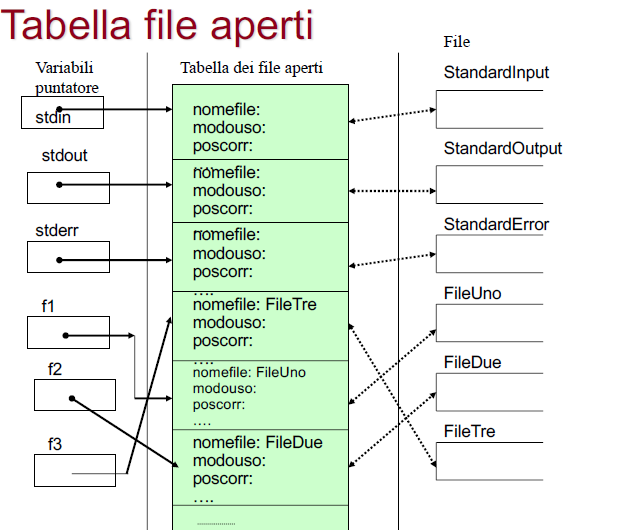
\includegraphics{C:/Users/giova/Documents/1_UNI/programmazione1/appunti/appunti-prog1/image/image-20201110122807433.png}

\hypertarget{operazione-di-gestione-dei-file}{%
\subsubsection{Operazione di gestione dei
file:}\label{operazione-di-gestione-dei-file}}

\begin{lstlisting}[language=C]
FILE *fopen (nomefile, modalità);
// Header della funzione fopen apri lo strem con un file <nomefile> e con modalità (vedi dopo)

int fclose (FILE *fp);
// Header della funzione che termina l'associazione tra il flusso e file di una periferica

// Per usare questa funzione in un programma devo
FILE *fp;
fp = fopen("MioFile", "r"); 
//se il file è nella cartella in cui sto lavorando, mentre invece se ho bisogno di un file in un altra posizione devo selezionare tutto il percorso del file
\end{lstlisting}

Per esempio:

\begin{lstlisting}[language=C]
#include <stdio.h>
#include <stdlib.h>

int main(int argc, char *argv[]){
    FILE *fp;
    char c;
    
    fp = fopen("/tmp/MioFile.txt", "r");
    
    if (fp == NULL){
        printf("Il file non può essere aperto\n");
        exit(1);
    }
    
    fclose(fp);
}
\end{lstlisting}

In questo esempio si deve notare che:

\begin{enumerate}
\def\labelenumi{\arabic{enumi}.}
\item
  \passthrough{\lstinline!if (fp == NULL)!} è necessario a controllare
  che l'azione di apertura del file sia andata a buon fine, infatti in
  caso di errore il puntatore assume valore \emph{NULL}
\item
  Nel caso avvenga un errore è necessario che il programmi termini con
  \passthrough{\lstinline!exit()!} , prima di cercare di lavorare su una
  cosa che non esiste
\item
  ricordare \passthrough{\lstinline!fclose(<puntatore\_a\_file>)!} per
  chiudere la periferica. Attenzione alle operazioni di
  \passthrough{\lstinline!fflush()!} prima di chiudere. Questa funzione
  deve \textbf{SEMPRE ESSERE PRESENTE} alla fine, perché la sua mancanza
  può provocare perdita di dati, perdita di files e altri errori.
\end{enumerate}

\hypertarget{modalituxe0-di-accesso-ai-files}{%
\paragraph{Modalità di accesso ai
files}\label{modalituxe0-di-accesso-ai-files}}

Come visto sopra la funzione \passthrough{\lstinline!fopen()!} accetta
come secondo parametro la modalità con cui deve accedere al file. Le
modalità possibili sono:

\begin{itemize}
\tightlist
\item
  \passthrough{\lstinline!r!} : lettura modalità testo
\item
  \passthrough{\lstinline!w!} : scrittura modalità testo a inizio file
\item
  \passthrough{\lstinline!a!} : scrittura modalità testo alla fine del
  file (\emph{append})
\item
  \passthrough{\lstinline!rb!} : lettura in modo binario
\item
  \passthrough{\lstinline!ab!} : scrittura in modalità binaria a fine
  file (\emph{append})
\item
  \passthrough{\lstinline!wb!} : scrittura in modalità binaria a inizio
  file
\item
  \passthrough{\lstinline!r+!} : apertura per modalità testo per lettura
  e scrittura
\item
  \passthrough{\lstinline!w+!} : crea file in modalità testo per lettura
  e scrittura. Si il file già esisteva viene sovrascritto
\item
  \passthrough{\lstinline!a+!} : append o crea un file in modalità testo
  per lettura e scrittura a fine file
\item
  \passthrough{\lstinline!r+b!} : apertura in modalità binaria per
  lettura e scrittura
\item
  \passthrough{\lstinline!w+b!} : crea un file in modalità binario per
  scrittura e lettura
\item
  \passthrough{\lstinline!a+b!} : append o crea file in modalità binario
  per lettura e scrittura.
\end{itemize}

Ricordare che se un file è aperto in una modalità non si può usarne un
altra senza chiuderlo e riaprirlo.

\hypertarget{altre-funzioni-utili-alla-gestione-dei-file}{%
\paragraph{Altre funzioni utili alla gestione dei
file}\label{altre-funzioni-utili-alla-gestione-dei-file}}

Esistono funzioni per la lettura e scrittura di caratteri: (tutti
restituiscono \emph{EOF - end of file} in caso di errore)

\begin{lstlisting}[language=C]
int getchar (void); // legge da stdin

int putchar(int c); // scrive su stdout

int fget (FILE *fp); // legge carattere da FILE
  
int fputc (int c, FILE *fp); // scriver carattere su FILE
 
\end{lstlisting}

\emph{Per la lettura e scrittura di stringhe su file:}

\begin{lstlisting}[language=C]
char *fgets (char *s, int length, FILE *fp);

int *fputs (char *s, FILE *fp);

int puts(char *s);
 
\end{lstlisting}

\begin{itemize}
\tightlist
\item
  \passthrough{\lstinline!fgets()!} e \passthrough{\lstinline!fputs()!}
  scrive stringhe su \emph{stream} specificato, ad eccezione del
  carattere \emph{NULL}. Restituiscono \emph{EOF} come errore.
\item
  \passthrough{\lstinline!fgets()!} legge i caratteri finché non trova
  il \emph{EOF}, il valore nullo o al più
  \passthrough{\lstinline!length-1!}, il carattere
  \passthrough{\lstinline!\\n!} viene letto e incluso nella stringa
\item
  \passthrough{\lstinline!puts()!} scrive stringhe su \emph{stdout}
  aggiungendo \emph{NEWLINE} e restituisce \emph{EOF} come errore.
\end{itemize}

\emph{Operazioni sulla gestione dei files}

\begin{lstlisting}[language=C]
int remove (nomeFile);

int rename (vecchionome, nuovonome);
\end{lstlisting}

\begin{itemize}
\tightlist
\item
  le azioni \passthrough{\lstinline!remove()!} e
  \passthrough{\lstinline!rename()!} servono a rimuovere e rinominare i
  file.
\item
  entrambe queste funzioni dipendono dal sistema operativo: se non si
  dispongono i permessi necessari a accedere alle risorse e a modificare
  lo stato dei file, o se il file risulta aperto da un altro
  \emph{stream} allora l'azione non è consentita e si restituisce un
  errore.
\item
  il controllo dei permessi e dello stato di utilizzo del file è
  sottoposto all'implementazione delle funzioni, che devono prevedere
  questi due casi.
\end{itemize}

\emph{Operazione di lettura e scrittura di testo da/su file:}

\begin{lstlisting}[language=C]
int printf(stringa, elementi);                      // Scrittura in stdout

int scanf(stringa, indirizzo_elementi);             // Lettura in stdin

int fprintf(FILE *fp, stringa, elementi);           // Scrittura su stream di tipo FILE

int fscanf(FILE *fp, stringa, indirizzo_elementi);  // Lettura su stream tipo FILE
\end{lstlisting}

\emph{Operazione di lettura e scrittura in binario da/su file:}

\begin{lstlisting}[language=C]
int fread(void *ptr, dimElemento, numElementi, FILE *fp);

int fwrite(void *ptr, dimElemento, numElementi, FILE *fp);
\end{lstlisting}

\begin{itemize}
\tightlist
\item
  \passthrough{\lstinline!fread()!} legge un blocco di dimensione
  maggiore di un byte e li memorizza all'indirizzo di
  \passthrough{\lstinline!ptr!}. Restituisce il numero di elementi
  effettivamente letti, che potrebbe essere diverso da
  \passthrough{\lstinline!dimElemento*numElementi!}, quindi bisogna
  controllare con \passthrough{\lstinline!ferror()!} se sono ritornati
  errori.
\item
  \passthrough{\lstinline!fwrite()!} scrive blocchi di byte prelevandoli
  dall'indirizzo di \passthrough{\lstinline!ptr!}. Restituisce il numero
  di elementi effettivamente scritti, quindi sorge la possibilità di
  controllo anche in questo caso.
\end{itemize}

\emph{Accesso Random a FILE:}

\begin{lstlisting}[language=C]
int fseek(FILE *fp, long offset, int refpoint);

void rewind(FILE *fp);
\end{lstlisting}

\begin{itemize}
\tightlist
\item
  \passthrough{\lstinline!fseek()!} permette di accedere a posizioni nel
  file \passthrough{\lstinline!fp!} per operazioni di lettura e
  scrittura:

  \begin{itemize}
  \tightlist
  \item
    \passthrough{\lstinline!fp!} è il puntatore a tipo \emph{FILE}
  \item
    \passthrough{\lstinline!refpoint!} è il parametro che indica da dove
    bisogna calcolare l'\passthrough{\lstinline!offset!}. Questo
    parametro può variare tra:

    \begin{itemize}
    \tightlist
    \item
      \passthrough{\lstinline!SEEK\_SET!}: l'inizio del file
    \item
      \passthrough{\lstinline!SEEK\_CUR!}: posizione corrente del
      cursore, cioè l'elemento incaricato di scorrere lo stream
    \item
      \passthrough{\lstinline!SEEK\_END!}: fine del file
    \end{itemize}
  \item
    \passthrough{\lstinline!offset!} è il numero di bytes per il calcolo
    della nuova posizione corrente a partire da
    \passthrough{\lstinline!refpoint!}
  \end{itemize}
\item
  da notare che la funzione \passthrough{\lstinline!rewind()!} non è
  altro che la funzione macro per eseguire
  \passthrough{\lstinline!fseek(fp, 0, SEEK\_SET)!}, cioè iniziale a
  leggere lo stream dall'inizio con \emph{offset} uguale a zero.
\end{itemize}

\hypertarget{pro-e-contro-di-file-binari-e-di-testo}{%
\paragraph{Pro e Contro di File Binari e di
Testo}\label{pro-e-contro-di-file-binari-e-di-testo}}

Entrambi i tipi di file hanno lati positivi e negativi:

\emph{FILE BINARI:}

\begin{itemize}
\tightlist
\item
  \emph{PRO}: occupano meno spazio, hanno la possibilità di un accesso
  random
\item
  \emph{CONTRO}: non c'è portabilità tra calcolatore, non si può leggere
  con un normale editor di testo
\end{itemize}

\emph{FILE di TESTO:}

\begin{itemize}
\tightlist
\item
  \emph{PRO}: completa portabilità fra calcolatori
\item
  \emph{CONTRO}: più complicata la modifica e l'accesso random, perché
  bisogna conoscere la struttura del file, dimensione maggiore a parità
  di contenuto, possibilità di corruzione e incompatibilità dei
  caratteri
\end{itemize}

\hypertarget{gestione-degli-errori}{%
\subsubsection{Gestione degli errori}\label{gestione-degli-errori}}

Durante l'utilizzo dei files, si possono causare degli errori. Questi
devono essere correttamente gestiti per evitare un comportamento non
corretto del programma.

Quando la funzione deve restituire una variabile di tipo \emph{FILE},
c'è la possibilità di un errore generico nell'inizializzazione dello
stream, ovvero quando si restituisce il puntatore con un valore
\emph{NULL}, e la possibilità di raggiungere l'\emph{EOF}, quindi
terminare la lettura del file.

Per controllare e in caso prevenire questi errori, sono presenti tre
funzioni:

\begin{lstlisting}[language=C]
int ferror(FILE *fp);     // return TRUE se errore in un azione di r/w

int feof(FILE *fp);      // return TRUE se viene raggiunta la fine del file

void clearerr(FILE *fp); // esegue la cancellazione dei segnali di errore
\end{lstlisting}

\hypertarget{programmazione-ricorsiva}{%
\subsection{Programmazione Ricorsiva}\label{programmazione-ricorsiva}}

da recuperare appunti dal tablet

\hypertarget{allocazione-dinamica}{%
\subsection{Allocazione dinamica}\label{allocazione-dinamica}}

L'allocazione normalmente avviene in maniera statica, ovvero conosco la
dimensione in partenza e con questa informazione creo uno spazio di
memoria che possa contenere queste informazioni. Questo limite nella
quantità però può essere un limite, ad esempio in una variabile che deve
gestire un input:

\begin{itemize}
\tightlist
\item
  se ho una variabile troppo piccola c'è il rischio di \emph{overflow},
  ovvero di riempirla troppo e in caso causare un crash del programma o
  un comportamento anomalo
\item
  se ho una variabile troppo grande rischio di occupare un sacco di
  spazio per niente, togliendolo invece a altri processi a cui potrebbe
  servire.
\end{itemize}

Questo quindi riporta il problema alle capacità del programmatore, che
dovevano essere molto bravi a stimare la quantità di memoria corretta.
Ma in realtà per risolvere questo problema in un modo molto più elegante
si può usare la programmazione con tipi di dato a memoria dinamica,
ovvero creare oggetti che non possono essere descritti in modo statico
dal programma. Questo può servire anche nel caso la variabile sia vuota,
e quindi ci sia la necessità di liberare completamente lo spazio.

Nel C queste funzioni sono presenti nella
\passthrough{\lstinline!<stdlib.h>!}, una libreria che contiene la
strategia per un allocazione e de-allocazione della memoria dinamica. Si
interfaccia con le risorse del sistema operativo e si occupa della
richiesta e del rilascio della memoria.

Ricordo che di solito le variabili vengono allocate all'inizio del
programma e viene de-allocata alla fine dell'esecuzione del programma.
Tutte queste operazioni, insieme ai record di attivazione sono presenti
nello stack, ovvero quella struttura che si occupa della gestione delle
funzioni.

Nel C questa libreria ha una funzione nativa che si occupa
dell'allocazione dinamica:

\begin{lstlisting}[language=C]
void * malloc(size_t size); // Header della funzione malloc
\end{lstlisting}

In cui il parametro formale è di tipo \passthrough{\lstinline!size\_t!}
che praticamente è un \passthrough{\lstinline!unsigned int!}. La
funzione torna un puntatore alla sezione di memoria assegnata, ma questo
puntatore è sprovvisto di tipo, che va quindi assegnato al momento del
ritorno della funzione attraverso un casting.

Il suo funzionamento è il seguente:

\begin{lstlisting}[language=C]
#include <stdlib.h>

int main(){
    
    int *P; // Definisco un puntatore a intero
    
    P = malloc(sizeof(int));
}
\end{lstlisting}

L'operazione che si sta eseguendo è di \emph{portabilità}, infatti così
facendo si può definire la quantità di byte per il tipo \emph{int} su
ogni macchina che il codice viene eseguito, rendendo il codice stesso
molto flessibile.

Nell'esempio bisogna notare che:

\begin{enumerate}
\def\labelenumi{\arabic{enumi}.}
\tightlist
\item
  viene lanciata la funzione \passthrough{\lstinline!malloc!} che si
  occupa di creare uno spazio di memoria della dimensione passata, in
  questo caso la dimensione è \passthrough{\lstinline!sizeof(int)!}.
\item
  La funzione \passthrough{\lstinline!sizeof()!} restituisce il valore
  intero di byte che un certo tipo di dato necessita. Può sembrare
  inutile nel caso di un valore \emph{int}, di cui è conosciuta la
  dimensione, ma risulta molto comoda quando abbiamo un tipo di dato
  user-defined.
\item
  La funzione \passthrough{\lstinline!malloc!} torna un indirizzo alla
  posizione di memoria in cui è stato creato lo spazio per la variabile.
  È molto importante che il puntatore sia definito dello stesso tipo di
  dato di cui si sta creando lo spazio di memoria, in modo che il
  compilatore riesca a ``tradurre'' quello che è contenuto in
  quell'indirizzo.
\end{enumerate}

Potrebbe succedere che questa assegnazione di memoria non vada a buon
fine, e quindi devo verificare che il puntatore non torni \emph{NULL}.
Se si trova il valore nullo del puntatore però si sa che non si è
assegnata la memoria, ma non se ne conosce il motivo.

Dopo queste operazioni, però bisogna ricordare di rilasciare la memoria
quando si smette di usarla. Se non si rilascia una zona di memoria non
avvengono errori di sintassi, però potrebbe succedere che il sistema
operativo si rifiuti di fornirci altra memoria poiché ne abbiamo troppa
allocata e inutilizzata. Per eseguire questa operazione si esegue:

\begin{lstlisting}[language=C]
TipoPuntatore* P;
free(P);
\end{lstlisting}

In cui il puntatore è l'indirizzo alla zona di memoria che è stata
precedentemente allocata. Per questo è importante non perdere mai
l'indirizzo originale della zona di memoria creata, in modo che si possa
sempre de-allocare lo spazio.

\hypertarget{gestione-della-memoria-con-lallocazione-dinamica}{%
\subsubsection{Gestione della memoria con l'allocazione
dinamica}\label{gestione-della-memoria-con-lallocazione-dinamica}}

Sappiamo che generalmente le funzioni lavorano sulla struttura dello
\textbf{stack}, che contiene le variabili delle funzioni create
staticamente all'interno delle funzioni e i record di attivazione.
Questo spazio viene poi anche liberato automaticamente al momento della
fine della funzione, oppure alla fine del programma.

Quando invece si dichiarano tipi di dato in modo dinamico, il
compilatore ci assegna un tipo di memoria diversa chiamato
\textbf{heap}, cioè mucchio. Nello \emph{stack} quindi compariranno dei
puntatori, che non saranno altro che gli indirizzi della memoria
allocata dinamicamente. Quest'ultima invece è posizionata
nell'\emph{heap}. La mappa della memoria usata nel nostro programma
quindi ora prende questa forma.

(L'esempio rappresenta lo \emph{stack} con i vari indirizzi che puntano
alla memoria dinamica posizionata nell'\emph{heap}, che a sua volta può
contenere un puntatore a altre zone allocate dinamicamente)

\begin{figure}
\centering
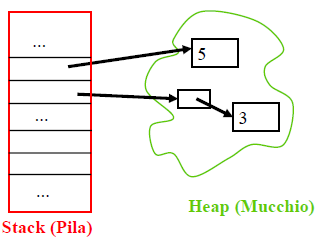
\includegraphics{C:/Users/giova/Documents/1_UNI/programmazione1/appunti/appunti-prog1/image/image-20210103130905695.png}
\caption{image-20210103130905695}
\end{figure}

Come si vede anche dalle foto, mentre lo \emph{stack} è molto ordinato,
l'\emph{heap} non è così uniforme perchè contiene dei blocchi di memoria
di grandezza diversa e generalmente i blocchi a disposizione gestiti
dall'allocazione dinamica \emph{non} sono in generale contigui.

La gestione della memoria nell'heap è molto complicata, perché bisogna
tener conto in un registro che zone di memoria sono occupate e quali
sono libere, oltre che segnalare il contenuto in quelle che sono piene.
Questo è importante perché il compilatore ha bisogno di sapere quali
zone sono libere o occupate in un certo momento per potere gestire il
rilascio della memoria.

Siccome la gestione dello spazio disponibile e quello occupato nell'heap
è molto complicato, si utilizza una struttura di dati chiamata
\emph{lista}. All'interno di questa lista sono presenti tutte le
informazioni che sono: le dimensioni dello spazio disponibile, le
informazioni necessarie ad aggiornare il registro delle zone libere e di
quelle occupate e un puntatore alla prossima zona libera.

I blocchi, cioè gli elementi della lista, sono tenuti in ordine
crescente di indirizzo e l'ultimo blocco punta al primo, crea quindi una
\emph{lista circolare}.

Per capire il funzionamento e il motivo di questa implementazione per la
gestione della memoria dell'heap, si deve spiegare il funzionamento
della \passthrough{\lstinline!malloc!}. Quando questa funzione viene
lanciata, il compilatore inizia a cercare una zona libera di memoria a
partire dal puntatore che rappresenta l'inizio degli indirizzi a
disposizione dell'heap (elemento 1). Da questo si scandaglia la lista
finché non si trova uno spazio disponibile, e quando lo si trova si
aggiorna il registro. Se nel corso di questa ricerca il puntatore torna
uguale a quello inziale, cosa possibile siccome la lista è circolare,
vuol dire che non sono presenti zone di memoria libere nel range, e
quindi si tornerà un errore.

\begin{figure}
\centering
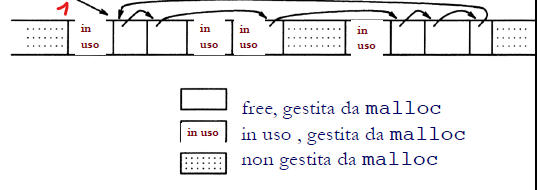
\includegraphics{C:/Users/giova/Documents/1_UNI/programmazione1/appunti/appunti-prog1/image/image-20210103234028124.png}
\caption{image-20210103234028124}
\end{figure}

In generale quindi la memoria necessaria al funzionamento del programma
è concettualmente semplificabile in questo modo:

\begin{figure}
\centering
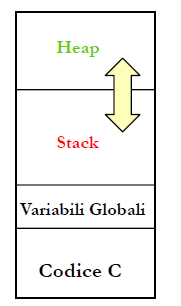
\includegraphics{C:/Users/giova/Documents/1_UNI/programmazione1/appunti/appunti-prog1/image/image-20210103234832110.png}
\caption{image-20210103234832110}
\end{figure}

Dove il \emph{codice C} contiene le istruzioni in parte alle
\emph{variabili Globali}, che sono visibili a tutto il programma. Poi
nello \emph{stack}, si posiziona al gradino più basso sempre la funzione
\emph{main}, e seguono poi tutti le altre contenenti anche tutti i
record di attivazione necessari a quella determinata funzione. Infine la
zona dell'heap. Questo stack può aumentare l'altezza nel programma,
analogamente l'heap, che può anche lui cambiare dimensione (questo è il
motivo per cui c'è la freccia gialla).

Si ricorda poi che è possibile dichiarare la sezione di memoria dinamica
allocata come variabile \emph{static} e quindi evitare che questa
determinata zona di memoria venga creata tutte le volte che si entra
nella funzione che la richiede, ma al contrario, sia creata alla
partenza del programma e poi utilizzata per tutto il suo svolgimento.
Questo può essere utile se si vuole evitare di dichiarare molte volte
zone di memoria molto grandi.

\hypertarget{rischi-nella-gestione-dinamica-della-memoria}{%
\subsubsection{Rischi nella gestione dinamica della
memoria}\label{rischi-nella-gestione-dinamica-della-memoria}}

Tra i maggiori rischi dell'uso di programmazione con uso della memoria
dinamica è la produzione di \emph{garbage}. La parola garbage è
esemplificativa del fatto che si produce della memoria che non viene
utilizzata, ma che è rimasta allocata. Questo avviene spesso quando si
perde il puntatore alla zona di memoria dinamicamente allocata. Il
\emph{garbage} quindi viene creato semplicemente per opera del
programmatore, che compie degli sbagli al momento dell'assegnazione e
del rilascio di memoria dinamica.

Un altro errore piuttosto comune è il \emph{dangling reference}, cioè un
\emph{assegnazione fluttuante}. Succede ad esempio quando un luogo di
memoria è indicato da due puntatori e si esegue una
\passthrough{\lstinline!free!} per liberare la zona con uno dei due. Il
problema che eseguendo la funzione \emph{solo} un puntatore verrà
eliminato, mentre il suo gemello si mantiene e adesso indica una zona di
memoria vuota, perché è stata de-allocata.

Questo può avere lati negativi sulla correttezza del risultato
aspettato, e alcuni linguaggi hanno tolto questa funzionalità.

\hypertarget{garbage-collection}{%
\paragraph{Garbage Collection}\label{garbage-collection}}

Il problema dei \emph{dangling reference} è facilmente risolvibile
attraverso una tecnica chiamata \textbf{garbage collection}, che
consiste nella raccolta di zone di memoria non referenziate. Per il
C/C++ esistono librerie ad-hoc.

Altri linguaggi di alto livello come LISP o JAVA hanno un sistema di
garbage collection nativamente.

Ci sono anche altre tecniche per risolvere questo problema, come
l'\emph{Automatic Reference Counting} o \emph{ARC}. Questo modo di fare
è utilizzato ad esempio nell'Objective-C e nel Swift (linguaggi
ecosistema Apple). L'ARC funziona in modo che tiene conto degli oggetti
di memoria referenziati, e quando navigando la lista ne trovano uno non
referenziato cambiano l'indicazione da occupato a libero.

\hypertarget{allocazione-dinamica-nel-c}{%
\subsubsection{Allocazione dinamica nel
C++}\label{allocazione-dinamica-nel-c}}

L'operatore che crea un blocco di memoria dinamica nel C++ è la funzione
\passthrough{\lstinline!new!}, che general dinamicamente una variabile
di un certo tipo assegnandole un blocco di memoria della dimensione
opportuna e restituisce il puntatore che contiene l'indirizzo al blocco
appena creato.

La sintassi completa è:

\begin{lstlisting}[language={C++}]
tipoPuntatore *ptr = new tipoPuntatore;
tipoPuntatore *ptr = new tipoPuntatore[3];

// ad esempio per creare lo spazio dinamico di 100 caratteri:

char* p = new char[100];

// Per liberare la memoria nel C++ si utilizza (singolo pointer o array di elementi)
delete ptr;
delete [] ptr; 
\end{lstlisting}

\hypertarget{tipi-di-dato-astratto}{%
\subsection{Tipi di Dato Astratto}\label{tipi-di-dato-astratto}}

Come abbiamo visto i tipi di dato sono l'insieme di valori di una
variabile.

L'\emph{Abstract Data Type} è un modello matematico che include le
operazioni definite nel modello assieme al tipo di dato. Il concetto di
\emph{ADT} esula dal linguaggio di programmazione perché sono cose che
possono essere implementate in ogni linguaggio. Gli \emph{ADT} invece
hanno la necessità di usare strutture proprie di un linguaggio di
programmazione per essere creati, di conseguenza la loro implementazione
è differente.

\hypertarget{liste-concatenate}{%
\subsubsection{Liste concatenate}\label{liste-concatenate}}

Se bisognava gestire una sequenza di valori in ingresso fin ad ora
l'unico modo per rappresentarli era l'utilizzo di un array. Nel caso
però che ci si chieda un insieme dinamico di elementi, però, il concetto
di array non funziona perché non riesce a gestire un insieme dinamico di
elementi.

Ma adesso possiamo anche usare le \textbf{liste concatenate} come
soluzione alternativa per creare un insieme di elementi \emph{quando
l'accesso casuale non è un requisito necessario}.

Nella lista concatenata i blocchi che la compongono possono anche essere
in zone di memoria distanti, perché sono allocati nell'heap. E già qui
ci si distanzia dal concetto di base dell'array, che consiste in una
serie di spazi tutti consecutivi.

Per implementare una coda è necessario che ogni elemento contenga almeno
le informazioni per accedere all'elemento successivo, ma nel caso di una
lista doppiamente concatenata, l'oggetto contiene anche il link
all'elemento precedente.

\hypertarget{vantaggi-e-svantaggi-rispetto-allarray}{%
\paragraph{Vantaggi e svantaggi rispetto
all'array}\label{vantaggi-e-svantaggi-rispetto-allarray}}

\begin{longtable}[]{@{}cc@{}}
\toprule
\begin{minipage}[b]{(\columnwidth - 1\tabcolsep) * \real{0.50}}\centering
VANTAGGI\strut
\end{minipage} &
\begin{minipage}[b]{(\columnwidth - 1\tabcolsep) * \real{0.50}}\centering
SVANTAGGI\strut
\end{minipage}\tabularnewline
\midrule
\endhead
\begin{minipage}[t]{(\columnwidth - 1\tabcolsep) * \real{0.50}}\centering
Flessibilità di modifica\strut
\end{minipage} &
\begin{minipage}[t]{(\columnwidth - 1\tabcolsep) * \real{0.50}}\centering
Onerosità dell'accesso agli elementi, cioè ho un unico modo per accedere
a un determinato elemento e questo modo è di scorrere tutta la
lista\strut
\end{minipage}\tabularnewline
\begin{minipage}[t]{(\columnwidth - 1\tabcolsep) * \real{0.50}}\centering
Riduzione e aumento dinamico delle dimensioni\strut
\end{minipage} &
\begin{minipage}[t]{(\columnwidth - 1\tabcolsep) * \real{0.50}}\centering
Non ho un accesso casuale ai dati (come invece l'array)\strut
\end{minipage}\tabularnewline
\begin{minipage}[t]{(\columnwidth - 1\tabcolsep) * \real{0.50}}\centering
Memorizzo solo quello che serve, non ho bisogno di sovradimensionare e
non rischio di sottodimensionare\strut
\end{minipage} &
\begin{minipage}[t]{(\columnwidth - 1\tabcolsep) * \real{0.50}}\centering
\strut
\end{minipage}\tabularnewline
\bottomrule
\end{longtable}

\hypertarget{modello-matematico-dietro-le-liste-concatenate}{%
\paragraph{\texorpdfstring{Modello matematico dietro le \emph{liste
concatenate}}{Modello matematico dietro le liste concatenate}}\label{modello-matematico-dietro-le-liste-concatenate}}

La lista è una sequenza di zero o più elementi di un determinato tipo di
dato, anche strutturato se necessario.

Il numero di elementi (\emph{n}) di tale lista è detta \emph{lunghezza}.
Se \passthrough{\lstinline!n >= 1!}, \emph{a1} è il primo elemento
dell'insieme. Se \passthrough{\lstinline!n=0!} la lista è vuota. La
lista procede in ordine lineare, quindi \emph{a1} viene prima di
\emph{a2} e così via. Inoltre l'accesso è sequenziale quindi da un
elemento posso passare solo al suo successivo o precedente, non posso
``saltare''. Essendo un insieme dinamico posso partire con zero elementi
al suo interno e poi farla crescere o decrescere.

E' utile definire l'esistenza di un blocco \emph{FINE}. Creandolo, la
\emph{distanza} è il numero di elementi tra il primo blocco e il blocco
\emph{FINE}, e varierà nel tempo.

\hypertarget{implementazione}{%
\paragraph{Implementazione}\label{implementazione}}

L'implementazione in C necessita dell'utilizzo di una variabile
strutturata:

\begin{lstlisting}[language=C]
typedef struct Telemento{
    Tipoelemento info;
    struct EL *Prossimo;
}Telemento;
\end{lstlisting}

All'interno di questa struttura dobbiamo notare la struttura
\emph{autoreferenziata} \passthrough{\lstinline!struct EL * Prossimo!}
che ci permette di raggiungere il prossimo elemento della lista. Questa
definizione è una forma di ricorsione. Quando si alloca l'oggetto il
calcolo dello spazio necessario però non cade in un loop infinito perché
gli elementi sono concatenati attraverso un puntatore a un elemento, non
l'intero elemento e quindi possiede un valore di memoria fisso.

Il campo \passthrough{\lstinline!struct EL *Prossimo!} è chiamato link e
viene usato per legare una struttura di \passthrough{\lstinline!EL!} a
una struttura dello stesso tipo. Inoltre questo puntatore è necessario a
contenere le informazioni necessarie per passare al prossimo elemento.

La rappresentazione di una lista quindi può essere una cosa del tipo:

\begin{figure}
\centering
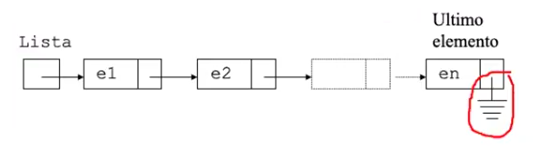
\includegraphics{C:/Users/giova/Documents/1_UNI/programmazione1/appunti/appunti-prog1/image/image-20201130102437198.png}
\caption{image-20201130102437198}
\end{figure}

Nella rappresentazione il simbolo della messa a terra segnala l'ultimo
elemento della lista, mentre il primo è chiamato \emph{testa}. L'ultimo
puntatore viene inizializzato a \passthrough{\lstinline!NULL!} e serve a
indicare che siamo arrivati alla fine della lista. La \emph{testa} della
lista, che può essere anche \passthrough{\lstinline!NULL!} se la lista è
vuota, di solito contiene il puntatore al primo elemento della lista.
Per trovare l'ultimo elemento quindi bisognerà scorrere la lista finché
non si raggiunge un elemento con \passthrough{\lstinline!prox == NULL!}.

Dopo aver definito il tipo di dato necessario a creare un blocco della
lista, attraverso i \passthrough{\lstinline!typedef!} creiamo degli
alias che potranno tornarci utili nella scrittura del programma. (Uno
che indica il singolo blocco della lista e l'altro che indica l'elemento
\emph{testa} della lista)

\begin{lstlisting}[language=C]
typedef struct EL ELemLista;
typedef ElemLista *ListaDiElem; 
\end{lstlisting}

Per dichiarare la lista poi si può fare:

\begin{lstlisting}[language=C]
ListadiElem Lista1, Lista2, Lista3; // Dichiarazione standard

ElemLista *Lista1;                  // Dichiarazione abbreviata

struct EL *Lista1;                  // Dichiarazione con NomeTipo completo
\end{lstlisting}

La dichiarazione standard mette in evidenza che si sta dichiarando una
lista, la dichiarazione abbreviata mette in evidenza il tipo di blocchi
che conterrà la lista, mentre invece la dichiarazione con il nome del
tipo di dato completo permette di indicare esplicitamente il tipo dei
suoi elementi, senza ricorrere a un \passthrough{\lstinline!typedef!}
(che però è molto comodo nell'uso).

Per inizializzare una lista si deve creare il primo elemento, ovvero la
\emph{testa della lista} e assegnarci il valore
\passthrough{\lstinline!NULL!}.

\begin{lstlisting}[language=C]
ListaDiElem Lista;
Lista = NULL; 
\end{lstlisting}

Facendo questo si viene a creare un oggetto rappresentabile in questo
modo:

\begin{figure}
\centering
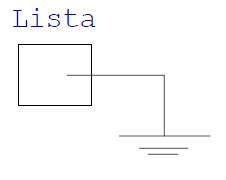
\includegraphics{C:/Users/giova/Documents/1_UNI/programmazione1/appunti/appunti-prog1/image/image-20210104114122777.png}
\caption{image-20210104114122777}
\end{figure}

Un altro modo di inizializzare la lista è dichiarare una testa in modo
globale e creare una funzione apposita per crearla. \emph{L'OPERAZIONE
DI ACCESSO ATTRAVERSO UNA VARIABILE GLOBALE è SCONSIGLIATO}:

\begin{lstlisting}[language=C]
#include <stdlib.h>
ListaDiElem Lista; // dichiaro globalmente
void Inizializza(void){
    Lista = NULL;
}
\end{lstlisting}

Un metodo migliore per eseguire questa operazione, è attraverso un
\emph{doppio puntatore}, ovvero un puntatore all'indirizzo della testa
della lista, che devo inizializzare a puntare a \emph{NULL}.

\begin{lstlisting}[language=C]
void initializza(ListaDiElem *ListaPtr){
    *ListaPtr = NULL;    
}
\end{lstlisting}

Il concetto di come lavora questa funzione è rappresentabile con:

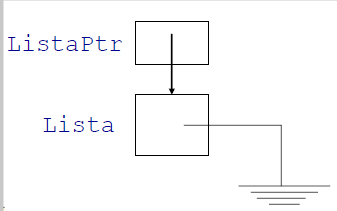
\includegraphics{C:/Users/giova/Documents/1_UNI/programmazione1/appunti/appunti-prog1/image/image-20210104114814838.png}

Dopodichè, ho bisogno di una serie di funzioni per la corretta
implementazione di questo \emph{ADT}. Queste funzioni sono:

\begin{itemize}
\item
  la funzione per il controllo se la lista è vuota

\begin{lstlisting}[language=C]
bool IsListaVuota(ListaDiElem Lista){

    if (Lista == NULL) return true;
    else return false;
}

// o anche

bool IsListaVuota(ListaDiElem Lista){
    return (Lista == NULL);
}
\end{lstlisting}

  \begin{itemize}
  \tightlist
  \item
    La funzione passa l'elemento per copia, siccome è necessario
    controllare solo il primo elemento della lista, che è un valore
    finito
  \item
    Il secondo metodo implica il fatto che la funzione abbia bisogno di
    far tornare un valore di tipo \passthrough{\lstinline!bool!} e
    quindi esegue un casting dopo aver eseguito il controllo.
  \end{itemize}
\item
  Funzione di ricerca di un elemento

\begin{lstlisting}[language=C]
bool Ricerca(ListaDiElem Lista, TipoElemento ElemCercato){

    ElemLista *Cursore;
    if (Lista != NULL){
      cursore = Lista;

        while (cursore != NULL){

            if (cursore->info == ELemCercato) return True;
            cursore = cursore->prox;

      }
    }
    return false; 
}
\end{lstlisting}

  \begin{itemize}
  \tightlist
  \item
    dichiaro un elemento \passthrough{\lstinline!Cursore!} che è un
    oggetto dello stesso tipo del blocco della lista e servirà per
    spazzolare tutti gli elementi di una lista
  \item
    con il controllo \passthrough{\lstinline"Lista != NULL"} controllo
    di non essere arrivato all'ultimo elemento
  \item
    nel ciclo \passthrough{\lstinline!while!} controllo se il mio
    elemento è quello cercato, se non lo è passo all'elemento
    successivo. Se trovo l'elemento cercato ritorno
    \passthrough{\lstinline!true!}. (quindi questa funzione permette di
    trovare solo il primo elemento, non calcola la possibilità di avere
    una ripetizione)
  \item
    se \passthrough{\lstinline!return false!} vuol dire che ho passato
    tutta la lista fino all'elemento che punta a
    \passthrough{\lstinline!NULL!} e non ho trovato nulla
  \item
    \emph{Questo algoritmo è molto influenzabile dalla quantità di
    elementi che sono presenti nella lista}
  \end{itemize}
\item
  Funzione di ricerca attraverso la ricorsione:

\begin{lstlisting}[language=C]
bool RicercaRecursiva(ListaDiElem Lista, TipoElemento ElementoCercato){

    if (Lista == Null) return false;
    else
        if (Lista->info == ELemCercato)
            return true;
      else
            return RicercaRicorsiva(Lista->Prox, ElemCercato);
}
\end{lstlisting}

  \begin{itemize}
  \tightlist
  \item
    \passthrough{\lstinline!Lista == NULL!} è per controllare di non
    essere arrivati all'ultimo elemento della lista, e questo passaggio
    è anche il \emph{passo base} della funzione ricorsiva
  \item
    Cerco l'elemento che voglio trovare con
    \passthrough{\lstinline!Lista->info == ElemCercato!} , se si trova
    torna \passthrough{\lstinline!true!}, mentre se non si trova si
    rilancia la funzione in maniera ricorsiva sul prossimo elemento
  \item
    Il numero di confronti con la funzione di ricerca non ricorsiva è lo
    stesso, ma il record di attivazione è molto maggiore, e aumenta di
    molto quando l'elemento cercato è molto distante dalla testa.
  \item
    si può fare anche un'implementazione con una funzione che torni
    l'elemento cercato quando viene trovato
  \end{itemize}
\item
  Due funzioni minori sono quella che ritorna il valore del primo
  elemento, e quella che torna il valore dell'ultimo elemento:

\begin{lstlisting}[language=C]
TipoElemento TestaLista(ListaDiElem Lista){
    if IsListaVuota(Lista) return TipoElemento();
    return Lista->prossimo->info;
}

ListaDiElem CodaLista(ListaDIElem Lista){
    if IsListaVuota(Lista) return NULL;
    return Lista->prossimo->prossimo;
}
\end{lstlisting}

  \begin{itemize}
  \tightlist
  \item
    In \passthrough{\lstinline!TestaLista!} controllo se la lista non è
    vuota, in caso torno un elemento vuoto (usando un costruttore),
    invece se non è vuota, torno il campo info del primo valore
  \item
    \passthrough{\lstinline!CodaLista!} ritorna il valore
    \passthrough{\lstinline!NULL!}se la lista è vuota, mentre torna il
    valore \passthrough{\lstinline!prossimo!} del primo elemento della
    lista, cioè il secondo elemento della lista.
  \end{itemize}
\item
  La funzione inserimento in testa è particolare delle lista, perché
  impiega sempre lo stesso tempo a essere eseguita:

\begin{lstlisting}[language=C]
void InsiementoInTesta(ListaDiElem *Lista, TipoElemento Elem){

    ElemLista *Punt;
    Punt = malloc(sizeof(ElemLista));
    Punt->info = Elem;

    Punt->prox = Elem;
    *Lista = Punt;

}
\end{lstlisting}

  \begin{itemize}
  \tightlist
  \item
    il funzionamento di base è che si crea un elemento nuovo, si impone
    il campo \passthrough{\lstinline!prossimo!} come il primo elemento
    della lista e si impone il puntatore a testa al primo elemento della
    lista.
  \item
    L'operazione ha un \emph{costo unitario e costante} per cui è un
    azione da prediligere
  \end{itemize}
\item
  Funzione inserimento in coda:

\begin{lstlisting}[language=C]
void InserisciInCoda(ListaDiElem *Lista, TipoElemento Elem){

    ElemLista *Ptr;

    if (ListaVuota (*Lista)){
        Ptr = malloc(sizeof(ElemLista));
        Ptr->Prox = NULL;
        Ptr->Info = Elem;
        *Lista = Ptr;
    }
    else InserisciInCoda(&((*Lista)->Prox), Elem);
}
\end{lstlisting}

  \begin{itemize}
  \tightlist
  \item
    la funzione lavora in modo ricorsivo finché non arrivo alla funzione
    di base, cioè finché non arrivo all'ultimo elemento
  \item
    a questo punto recupero l'elemento precedente, e impongo il suo
    campo \passthrough{\lstinline!prossimo!} come indirizzo del nuovo
    elemento, e il campo \passthrough{\lstinline!prossimo!} del nuovo
    elemento come puntatore a \passthrough{\lstinline!NULL!}
  \item
    L'inserimento in coda ha un costo di risorse e di tempo variabile in
    base al numero di elementi della lista, che si contrappone al costo
    unitario dell'inserimento in testa
  \end{itemize}
\item
  Funzione inserisci in lista ordinata (dove sto inserendo i valori in
  modo che rispettino una relazione d'ordine tra di loro):

\begin{lstlisting}[language=C]
void InserisciInOrdine(ListaDiElem * Lista, TipoElemento Elem){

    ElemLista *Punt, *PuntCorrente, *PuntPrecedente;
    PuntPrecedente = NULL;
    PuntCorrente=*Lista;

    while ((PuntoCorrente != NULL) && (Elem > PuntoCorrente->Info)){
        PuntoPrecedente = PuntoCorrente;
        PuntoCorrente = PuntoCorrente->Prox;
    }

    Punt = malloc(sizeof(ElemLista));
    Punt->Prox = PuntCorrente;
    Punt->Info = Elem;

    if (PuntoPcedente != NULL) PuntoPrecedente->Prox = Punt;
      else *Lista=Punt;
}
\end{lstlisting}

  \begin{itemize}
  \tightlist
  \item
    attraverso due variabili di servizio tengo conto dell'elemento
    corrente e del successivo. Controllo che il mio valore non sia
    compreso tra questi due rispetto alla mia relazione d'ordine: se
    questo è vero allora si inserisce l'elemento, se invece risulta
    falso allora si scorre ancora la lista
  \item
    la cosa più difficile di questa funzione è mantenere l'ordine, senza
    perdere link tra gli elementi e senza scombinare un ordine che
    preesisteva
  \end{itemize}
\item
  Altre funzioni per l'implementazione delle lista che possono tornare
  utili sono ad esempio:

  \begin{itemize}
  \tightlist
  \item
    \passthrough{\lstinline!StampaDiTuttaLaLista!}, che si occupa di
    stampare tutti i valori \passthrough{\lstinline!info!} degli
    elementi che compongono la lista
  \item
    \passthrough{\lstinline!EliminaElemLista!}, che si occupa di
    eliminare un elemento all'interno della lista, che può essere
    all'inizio, in coda o in mezzo. Per implementare questa funzione:

    \begin{itemize}
    \tightlist
    \item
      si trova l'elemento da eliminare
    \item
      si stacca il puntatore precedente e lo si ricollega al blocco
      successivo a quello trovato
    \item
      si esegue un operazione di
      \passthrough{\lstinline!free(Elemento)!}
    \end{itemize}
  \item
    funzione per il calcolo della lunghezza della lista
  \item
    funzione per rovesciare l'ordine della lista
  \item
    funzione per concatenare due liste
  \end{itemize}
\end{itemize}

\hypertarget{estensione-al-concetto-di-lista-liste-doppiamente-concatenate}{%
\paragraph{\texorpdfstring{Estensione al concetto di lista: \emph{Liste
doppiamente
concatenate}}{Estensione al concetto di lista: Liste doppiamente concatenate}}\label{estensione-al-concetto-di-lista-liste-doppiamente-concatenate}}

Le \emph{liste doppiamente concatenate} hanno due puntatori, uno che
punta al \passthrough{\lstinline!prossimo!} elemento e uno che punta al
\passthrough{\lstinline!precedente!}.

\begin{lstlisting}[language=C]
struct EL{
    tipoelemento Info;
    struct EL *Prox;
    struct EL *Prec;
}; 

typedef struct EL ElemLista;
typedef ElemLista *Lista;
\end{lstlisting}

Questa implementazione ha il costo di essere più grande, perché occupa
più spazio in memoria, però ha il lato positivo di facilitare
l'inserimento e la cancellazione degli elementi.

Nelle liste doppiamente concatenate si possono eseguire tutte le
funzioni delle liste semplicemente concatenate, però bisogna ricordare
sempre dell'aggiornamento e la gestione de secondo puntatore.

\hypertarget{estensione-al-concetto-di-lista-liste-circolari}{%
\paragraph{\texorpdfstring{Estensione al concetto di lista: \emph{Liste
circolari}}{Estensione al concetto di lista: Liste circolari}}\label{estensione-al-concetto-di-lista-liste-circolari}}

Questa struttura è molto importante, tanto che viene usata per gestire
il \emph{registro dell'heap}. Questa struttura ha come testa il primo
elemento, e nessun elemento punta a \passthrough{\lstinline!NULL!},
perché l'ultimo elemento punta di nuovo alla testa.

\begin{lstlisting}[language=C]
struct EL{
    Tipoelemento Info;
    struct EL *prox;
}

typedef struct EL ElemLista;
\end{lstlisting}

\hypertarget{sommario-le-liste}{%
\paragraph{\texorpdfstring{Sommario: \emph{LE
LISTE}}{Sommario: LE LISTE}}\label{sommario-le-liste}}

Le liste sono un importante esempio di struttura dinamica che nel C
viene implementata attraverso puntatori (quindi un implementazione di
basso livello). Possono essere singolarmente o doppiamente concatenate,
ordinate o meno, circolari. Hanno una serie di aspetti positivi e
negativi:

\begin{longtable}[]{@{}cc@{}}
\toprule
\begin{minipage}[b]{(\columnwidth - 1\tabcolsep) * \real{0.50}}\centering
VANTAGGI\strut
\end{minipage} &
\begin{minipage}[b]{(\columnwidth - 1\tabcolsep) * \real{0.50}}\centering
SVANTAGGI\strut
\end{minipage}\tabularnewline
\midrule
\endhead
\begin{minipage}[t]{(\columnwidth - 1\tabcolsep) * \real{0.50}}\centering
efficienza della struttura dinamica della lista rispetto all'array: si
evita lo spreco di memoria e anche l'\emph{overflow}, ovvero l'eccessivo
riempimento\strut
\end{minipage} &
\begin{minipage}[t]{(\columnwidth - 1\tabcolsep) * \real{0.50}}\centering
Nella struttura c'è un \emph{overhead} ovvero un ingombro maggiore
dell'elemento per via dei puntatori che lo compongono\strut
\end{minipage}\tabularnewline
\begin{minipage}[t]{(\columnwidth - 1\tabcolsep) * \real{0.50}}\centering
Tempo necessario all'esecuzione delle funzioni per l'inserimento in coda
sempre costante\strut
\end{minipage} &
\begin{minipage}[t]{(\columnwidth - 1\tabcolsep) * \real{0.50}}\centering
La funzione di ricerca e di inserimento in coda è molto penalizzata
siccome si deve scorrere tutta la lista\strut
\end{minipage}\tabularnewline
\bottomrule
\end{longtable}

\hypertarget{stack}{%
\subsubsection{Stack}\label{stack}}

L'\emph{ADT} chiamata \textbf{stack} può essere anche chiamata
\emph{lista LIFO}, cioè \emph{Last In First Out}, o \emph{pushdown
list}.

L'\emph{ADT stack} si usa ad esempio per i record di attivazione delle
funzioni.

\hypertarget{modello-matematico-dietro-lo-stack}{%
\paragraph{\texorpdfstring{Modello matematico dietro lo
\emph{stack}}{Modello matematico dietro lo stack}}\label{modello-matematico-dietro-lo-stack}}

Il modello matematico che permette di caratterizzare questo tipo di dato
è una lista \emph{L} dove l'inserimento e l'estrazione degli elementi
avviene esclusivamente da un solo lato, ovvero l'alto (\emph{top/cima}).

Le operazioni consentite sono quindi quelle di
\passthrough{\lstinline!push()!} e di \passthrough{\lstinline!pull()!},
che servono rispettivamente a aggiungere in cime alla pila e a togliere
l'elemento in cima alla pila.

Questo è molto importante perché consente di avere l'unicità
sull'elemento da modificare al momento dell'estrazione dallo stack e
anche sulla posizione di inserimento di un prossimo elemento.

\hypertarget{implementazione-1}{%
\paragraph{Implementazione}\label{implementazione-1}}

Le operazioni standard consentite nella gestione dello stack, come
predetto nel modello matematico sono:

\begin{lstlisting}[language=C]
Push(PILA, elemento);
Pop(PILA); 
\end{lstlisting}

Dove:

\begin{itemize}
\tightlist
\item
  \passthrough{\lstinline!Push()!} si occupa di inserire nella pila
\item
  \passthrough{\lstinline!Pop()!} si occupa dell'operazione di
  \emph{pull}, ovvero di estrarre dalla pila. Si nota che questa
  funzione ha bisogno solo del parametro che indica la pila, perché
  l'elemento da estrarre è univoco.
\end{itemize}

Per la natura con cui è creato lo stack si riempie sempre dal basso e
poi lo si svuota estraendo gli elementi dall'alto.

Altre operazioni semplificano la gestione dello stack, come ad esempio:

\begin{itemize}
\tightlist
\item
  \passthrough{\lstinline!top(PILA)!} : funzione che restituisce la
  testa della pila
\item
  \passthrough{\lstinline!StackIsEmpty(PILA)!} : funzione che controlla
  se lo stack è vuoto
\item
  \passthrough{\lstinline!StackIsFull(PILA)!} : funzione che controlla
  se lo stack è pieno (*questa funzione è necessaria solo se si è
  implementato lo stack in maniera statica).
\end{itemize}

Un problema si può creare nel caso ci sia la necessità di recuperare un
elemento che non è posto il cima. Si crea quindi un array o uno stack
temporaneo che servirà a contenere tutti i valori estratti in ordine
finché non trovo il valore cercato. Quando trovo l'elemento cercato,
riporto tutti gli elementi all'interno dello stack attraverso operazioni
di \passthrough{\lstinline!push()!} e posso eliminare la struttura
temporanea.

Ricorda che le funzioni di \passthrough{\lstinline!push()!} e di
\passthrough{\lstinline!pop()!} hanno un costo temporale e di calcolo
unico, cioè costano sempre la stessa quantità di risorse e di tempo,
quindi si possono usare ad oltranza senza il rischio che il tempo di
esecuzione cresca troppo.

Principalmente si possono fare due tipi di implementazione: con l'array
e con le liste. Entrambi hanno lati positivi e lati negativi.

\hypertarget{implementazione-con-array}{%
\subparagraph{\texorpdfstring{Implementazione con
\emph{Array}}{Implementazione con Array}}\label{implementazione-con-array}}

L'implementazione attraverso un array dello stack ha la principale
caratteristica di aver uno spazio di memoria fissa. Questo per lo più è
uno svantaggio, perché lo stack è una struttura che tende a crescere e
decrescere nel corso del programma, quindi avere la dimensione fissata
ha un certo peso sul programma. Oltre a questo va gestito il caso in cui
lo stack sia pieno.

Le funzioni di base per un implementazione di una struttura stack con
array sono:

\begin{lstlisting}[language=C]
#define StackMAx 20 // dichiarazione della massima dimensione dello stack

struct Tipostack {
    int N;           // numero di elementi presenti nello stack al momento
    int s[StackMAx]; // elementi presenti nello stack
}Tipostack;

typedef struct TipoStack STack;     // Alias per le variabili strutturate
typedef struct Tipostack *StackPtr; // Puntatore a tipoStack

bool StackIsEmpty(StackPtr p){
    return (p->N == 0);
}

bool StackIsFull(StackPtr p){
    return (p->N == MAXP);
}

void Push(StackPtr, Tipoelemento Elem){
    if (StackIsFull(p)){
        exit();
    }
    p->s[p->N] = Elem;
    p->N=p->N+1;
}

int Pop(StackPtr p){
    if (StackIsEmpty(p)){
        exit();
    }
    p->N = p->N-1;
    return p->s[p->N];
}
\end{lstlisting}

All'interno di questa implementazione dobbiamo notare:

\begin{itemize}
\item
  la creazione di un \passthrough{\lstinline!TipoStack!} che serve per
  avere il controllo sul numero di elementi presenti all'interno dello
  stack e logicamente sul valore di quegli argomenti
\item
  le funzioni \passthrough{\lstinline!StackIsFull()!} e
  \passthrough{\lstinline!StackIsEmpty()!} che sono necessarie al
  controllo sulla quantità di elementi all'interno dello stack, siccome
  questo è di dimensione fissata
\item
  la funzione \passthrough{\lstinline!Push()!} che inserisce un elemento
  nello stack e aumenta il contatore di spazi, logicamente controllando
  che lo stack non sia pieno
\item
  la funzione \passthrough{\lstinline!Pop()!} che estrae un elemento
  dalla cima dello stack, cioè dal valore del contatore, ne diminuisce
  il valore e torna il valore estratto
\end{itemize}

\hypertarget{implementazione-con-le-liste}{%
\subparagraph{\texorpdfstring{Implementazione con le
\emph{Liste}}{Implementazione con le Liste}}\label{implementazione-con-le-liste}}

Implementare uno stack con le liste permette alla struttura di crescere
e decrescere in modo dinamico e indefinitamente grande (logicamente si
ricordano le limitazioni fisiche). Il problema di questa implementazione
è che la gestione può diventare molto complicata dal punto di vista
logico.

Un implementazione tipo della struttura stack con le liste ha queste
particolari funzioni:

\begin{lstlisting}[language=C]
struct stackNode{           // Dichiaro l'elemento base della lista
    TipoElemento info;
    struct stackNode *prox;
};

typedef struct stackNode StackNode; // Dichiaro gli alias 
typedef stackNode *StackNodePtr;

bool StackIsEmpty(StackNodePtr Node){
    if (Node == NULL) return true;
    else return false;
}
void PrintStack(StackNodePtr CurrentPtr){
    
    if (StackIsEmpty){
        cout << "Stack vuoto!" << endl;
        exit();
    } else {
        while (CurrentPrt != NULL){
            cout << CurrentPtr->info;
            CurrentPtr = CurrentPtr->prox;
        }
    }
   
}

void Push(StackNodePtr *TopPrt, TipoElemento Elem){
    
    StackNode *Punt;
    Punt = new StackNode;
    
    Punt->Info=Elem;
    Punt->prox=*TopPtr;
    *TopPtr = Punt;
      
}

TipoElemento Pop(StackNodePtr *TopPtr){
    
    StackNodePtr tmpPtr=*TopPtr;
    TipoElemento topvalue = (*TopPtr)->info;
    
    *TopPtr = (*TopPtr)->Prox;
    free(tmpPtr);
    
    return topvalue;
}
\end{lstlisting}

In questa implementazione dobbiamo notare: (L'implementazione è fatta
con dei doppi puntatori perché Riccardi ha fatto così. Si può fare anche
molto più semplicemente con un puntatore singolo sfruttando la struttura
della lista e le sue funzioni)

\begin{itemize}
\tightlist
\item
  si definisce una variabile struttura che contiene la struttura di base
  di un blocco della lista e si dichiarano
\item
  le funzioni \passthrough{\lstinline!StackIsEmpty()!} e
  \passthrough{\lstinline!PrintStack()!} non sono necessarie ma
  facilitano l'implementazione
\item
  la funzione \passthrough{\lstinline!Push()!} prende il nuovo elemento,
  crea un blocco di dimensione dinamica nello stack e gli inserisce
  l'elemento. Poi esegue le operazioni di inserimento in testa della
  lista
\item
  la funzione \passthrough{\lstinline!Pop()!} si occupa di eliminare
  l'elemento di testa (esattamente le stesse operazioni che si farebbero
  per una lista concatenata) e tornare il valore dell'elemento eliminato
\end{itemize}

\hypertarget{un-utilizzo-particolare-dello-stack-la-notazione-postfissa}{%
\paragraph{\texorpdfstring{Un utilizzo particolare dello stack: \emph{la
notazione
postfissa}}{Un utilizzo particolare dello stack: la notazione postfissa}}\label{un-utilizzo-particolare-dello-stack-la-notazione-postfissa}}

Nel nostro uso quotidiano usiamo la notazione \emph{infissa}, cioè
quella che usa le parentesi, ma che ha di negativo il fatto che ci può
essere un ambiguità di precedenza nell'esecuzione delle operazioni che
viene risolta parzialmente con le parentesi, ovvero con la creazione di
una tabella di priorità.

Per evitare l'utilizzo di questa tabella si può usare la \emph{notazione
postfissa}, chiamata anche \emph{notazione polacca}. I principali lati
positivi di questa notazione per la scrittura è che:

\begin{itemize}
\tightlist
\item
  è utile per il calcolatore infatti è un tipo di scrittura che la
  macchina la preferisce e con cui lavora. Usandola si evita un
  \emph{layer} di traduzione eseguito dal linguaggio di programmazione.
\item
  è apprezzata perché non ha ambiguità, quindi non ha bisogno di usare
  tabelle di precedenza e associatività, non lascia quindi spazio alla
  soggettività
\item
  ha come lato negativo che utilizza un implementazione attraverso
  \emph{stack}, che può risultare complicata
\end{itemize}

La traduzione da notazione infissa a postfissa è semplificabile in
questo algoritmo:

\begin{itemize}
\tightlist
\item
  leggo una stringa in notazione infissa, che può essere
  \passthrough{\lstinline!( 9 + ( 8 * 4 ) )!}
\item
  eseguo un continuo \passthrough{\lstinline!push()!} di tutti gli
  elementi della stringa:

  \begin{itemize}
  \tightlist
  \item
    se trovo un operatore lo inserisco nello \emph{stack}
  \item
    se trovo un numero lo stampo
  \item
    se trovo una parentesi aperta o uno spazio ignoro
  \item
    se trovo una parentesi chiusa eseguo un
    \passthrough{\lstinline!pull()!} dallo stack e lo stampo
  \end{itemize}
\end{itemize}

Otterrò quindi un comportamento uguale a questo:

Questa funzione può essere scritta in codice:

\begin{lstlisting}[language={C++}]
void infissa2postfissa(const char* e){
    // Alloca lo stack
    for (int i=0; e[i] != '\0'; ++i){ // se la stringa non è finita continua
        if ((e[i] == "(") || (e[i] == ' ')) continue;
        // se la stringa contiene una parentesi, ignora e vai avanti
        if (e[i] == ')')
            cout << pop(S);
        // se incontri la parentesi tonda estrai e esegui, ritorna il valore finale
        if ((e[i] == '-') || (e[i] == '*') || (e[i] == '+')
                            || (e[i] == '/'))
            Push(S, e[i]);
        // se contiene un operando inserisci in cima allo stack
        if ((e[i] >= '0') && (e[i] <= '9'))
            cout << e[i];
        // se incontriamo un numero lo stampiamo in output
    }
    // Free S
}
\end{lstlisting}

\hypertarget{coda-o-queue}{%
\subsubsection{Coda o Queue}\label{coda-o-queue}}

L'\emph{ADT} coda o queue è chiamata anche lista FIFO, cioè First In
First Out. Il concetto di coda nella programmazione non è accomunabile a
quello della vita reale, infatti ci sono un sacco di modi per fare delle
code. Nella programmazione invece ne esiste uno solo.

La struttura della coda ha per definizione due accessi con funzioni
diverse: la \emph{coda} e la \emph{testa} , che hanno il compito
rispettivamente di uscita e di ingresso. E è proprio questa
caratteristica che differenzia lo stack dalla coda. Di conseguenza
questa struttura funziona in modo molto lineare:

\begin{itemize}
\tightlist
\item
  l'inserimento avviene solamente dal lato della coda
\item
  l'estrazione avviene solamente da lato della testa
\end{itemize}

\hypertarget{implementazione-2}{%
\paragraph{Implementazione}\label{implementazione-2}}

La struttura della coda ha principalmente due operazioni formali che
permettono l'inserimento e la rimozione.

\begin{lstlisting}[language=C]
void Enqueue(TipoCoda Coda,TipoDato Dato); 

TipoDiDato Dequeue(TipoCoda Coda);

void CheckIfEmpty(TipoCoda Coda);
void PrintQueue(TipoCoda Coda);
\end{lstlisting}

\begin{itemize}
\tightlist
\item
  la funzione \passthrough{\lstinline!Enqueue()!} che prenda la funzione
  (e in alcune implementazioni è proprio chiamata)
  \passthrough{\lstinline!Put()!} e si occupa dell'inserimento dal lato
  della coda
\item
  la funzione \passthrough{\lstinline!Dequeue()!}che prende la funzione
  ( e può anche prendere il nome di) \passthrough{\lstinline!Get()!} e
  si occupa dell'estrazione dell'elemento in testa alla coda e di
  ritornarlo
\item
  altre due funzioni molto meno importanti ma che semplificano
  l'implementazione sono \passthrough{\lstinline!CheckIfEmpty()!} e
  \passthrough{\lstinline!PrintQueue()!}, che con il loro nome spiegano
  bene la loro funzione
\end{itemize}

Come lo stack si può implementare questa struttura con due modi
differenti: attraverso l'uso delle liste e con l'uso degli array.

\hypertarget{implementazione-con-liste}{%
\subparagraph{\texorpdfstring{Implementazione con
\emph{LISTE}}{Implementazione con LISTE}}\label{implementazione-con-liste}}

\begin{lstlisting}[language={C++}]
typedef struct Tnodo{
    TipoElemento info;
    Tnodo* next;
}Tnodo;

struct queue{
    EL *Head;
    EL *Tail;
}


typedef struct EL ElemLista;
typedef EL* ElemPtr;
typedef struct queue Queue;
typedef Queue *QueuePtr;

void Enqueue(QueuePtr qP, TipoElemento El){
    
    ElemPtr = new Elemlista;
    ElemPtr->info = El;
    
    qP->Tail = ElemPtr;
    ElemPtr->next = NULL;
    
}

TipoElemento Dequeue(QueuePtr qP){
    
    ElemLista el = qP->Head->info;
    QueuePtr tmp = qP->Head;
    qP->Head = qP->Head->Prox;
    delete [] tmp;
    
    return el;    
    
}
bool checkIfEmpty(QueuePtr qP);

/* primo inserimento, devo modificarli entrambi
 * Head-Tail -> Tnodo inserito
 * aggiungo un altro
 * head -> Tnodo -> Tnodo2 -> NUll, con Tail -> Tnodo2
 * 
 */
\end{lstlisting}

In questa implementazione bisogna notare:

\begin{itemize}
\tightlist
\item
  la variabile strutturata rappresenta il blocco di base della lista,
  che contiene al suo interno il valore dell'elemento e il puntatore al
  prossimo blocco, come da definizione per le liste
\item
  la struttura \passthrough{\lstinline!queue!} fornisce la testa e la
  coda della lista, inizializzati nel \emph{main} o in una funzione a
  parte
\item
  definisco degli alias per rendere il codice più leggibile
\item
  la funzione \passthrough{\lstinline!Enqueue()!} è il corrispettivo per
  inserimento in coda della lista, con l'unica differenza che in questo
  caso la struttura \passthrough{\lstinline!queue!} fornisce già il
  puntatore alla coda, quindi evita di fare un ciclo su tutta la
  struttura
\item
  la funzione \passthrough{\lstinline!Dequeue()!} si occupa di eliminare
  l'elemento in testa, impostare il nuovo elemento di testa nella
  struttura \passthrough{\lstinline!queue!} e poi liberare lo spazio del
  blocco. Questa funzione torna l'elemento eliminato
\end{itemize}

\hypertarget{implementazione-con-array-1}{%
\subparagraph{\texorpdfstring{Implementazione con
\emph{Array}}{Implementazione con Array}}\label{implementazione-con-array-1}}

L'implementazione del concetto di coda con la struttura array avviene
con l'importante concetto per cui la struttura è allocata staticamente.

A lato di questo tipo di implementazione invece esiste il concetto di
\emph{buffer o array circolare}, che è semplicemente un array con una
diversa gestione degli indici. In quest'ultima struttura si deve fare
attenzione a come viene calcolato l'elemento successivo che è
leggermente diverso da un normale array:

\begin{lstlisting}[language={C++}]
i = (i+1);            // Incremento normale in una coda di array
i = (i+1) % CodaSize; // Incremeneto in un arrai circolare

// i = Codasize-1 sarà l'ultimo elemento dell'array
// i = Codasize +1 Sarà il primo elemento dell'array
\end{lstlisting}

L'array circolare quindi impone che:

\begin{itemize}
\tightlist
\item
  attraverso la relazione \passthrough{\lstinline!(i+1) \% CodaSize!} si
  verifica se incrementare o ritornare a zero. Infatti la relazione con
  l'operatore di modulo può anche essere chiamata verifica della
  condizione di pienezza, infatti se
  \passthrough{\lstinline!i == CodaSize!} vuol dire che il resto è
  uguale a zero e che quindi il buffer torna al valore zero
\item
  date queste condizioni si può dedurre che
  \passthrough{\lstinline!i = Codasize - 1!} è l'ultimo elemento
  dell'array e \passthrough{\lstinline!i = Codasize + 1!} è il primo
  elemento dell'array
\item
  il \passthrough{\lstinline!front!} descrive un indice di valore uguale
  a zero
\item
  \passthrough{\lstinline!rear!} indica il prossimo elemento.
\item
  la coda è vuota quando \passthrough{\lstinline!fronte == rear!}
\item
  la coda è piena quando
  \passthrough{\lstinline!(rear+1) \% CodaSize == front!}
\end{itemize}

Un implementazione possibile del buffer circolare è con un valore usato
come \emph{sentinella} ovvero come indice per indicare che la coda è
piena. Questa implementazione ha bisogno quindi di una colonna con il
ruolo di sentinella, motivo per cui serve inizializzare un array con
dimensione \passthrough{\lstinline!CodaSize+1!} per usare questa
tecnica.

Un tipo di implementazione possibile per la coda con gli array può
essere:

\begin{lstlisting}[language={C++}]
TipoElemento info;
struct queue{
    int CodaSize; // contiene al max CodaSize-1
    int Front;
    int Rear;
    TipoElemento *s;
};
typedef struct queue Queue;
typedef Queue *QueuePtr;
QueuPtr Q;

// Togliere dalla coda, incrementa di uno l'indice Front.

// Quando aggiungo in coda sta crescendo l'indice Rear.

bool QueueIsEmpty(Q);
bool QueueIsFull(Q);

void Enqueue(QueuePtr pt, TipoElemento El);
TipoElemento Dequeue(QueuePtr pt);

void QueuePrint(QueuePtr Q); // ricordarsi che è circolare, quindi devo usare il modulo
\end{lstlisting}

\begin{itemize}
\tightlist
\item
  le funzioni sono praticamente uguali a quelle che faresti per gestire
  una lista, ma più facili dal punto di vista logico. Se si vuole usare
  il buffer circolare bisogna ricordare il metodo per incrementarlo
  correttamente e implementarlo nel modo giusto.
\end{itemize}

\hypertarget{loperatore-xor-or-esclusivo}{%
\subsection{\texorpdfstring{L'operatore \emph{XOR (OR
esclusivo)}}{L'operatore XOR (OR esclusivo)}}\label{loperatore-xor-or-esclusivo}}

L'operatore \emph{XOR}, rappresentabile anche con il simbolo
\passthrough{\lstinline!⨁!} o il simbolo \passthrough{\lstinline!\^!},
rappresenta quello che nel linguaggio naturale è ``o uno o l'altro''.

\begin{longtable}[]{@{}lll@{}}
\toprule
A & B & X\tabularnewline
\midrule
\endhead
0 & 0 & 0\tabularnewline
1 & 1 & 0\tabularnewline
1 & 0 & 1\tabularnewline
0 & 1 & 1\tabularnewline
\bottomrule
\end{longtable}

Questo simbolo ha anche proprietà associative:

\begin{itemize}
\item
  \passthrough{\lstinline!A \^ B \^ C = (A \^ B) \^ C = A \^ (B \^ C)!}
\item
  \passthrough{\lstinline!A \^ 0 = A : A \^ A = 0!}
\end{itemize}

Questo simbolo può essere usato ad esempio per scambiare due variabili
senza la variabile temporanea:

\begin{lstlisting}[language={C++}]
tmp = x;
x = y;
y = tmp;

// usando l'operatore XOR
// x == A; y == B;
x = x ^ y; // x == A ^ B, y == B
y = x ^ y; // y == (A ^ B) ^ B
           //   == A ^ (B ^ B)
           //   == A ^ 0 == A
           
x = x ^ y; // x == (A ^ B) ^ A 
           //   == (A ^ A) ^ B

// Alla fine delle 3 assegnazioni si ottiene lo scambio di variabili senza variabile tmp. Queste sono operazioni a livello di bit.
\end{lstlisting}

\hypertarget{algoritmi-di-ricerca-e-ordinamento}{%
\subsection{Algoritmi di Ricerca e
Ordinamento}\label{algoritmi-di-ricerca-e-ordinamento}}

Lo scopo di un algoritmo di ricerca o di ordinamento è che eseguano
l'operazione nel miglior modo possibile, nel minor tempo possibile e
senza compiere errori. Questi tre punti sono molto difficili da
mantenere assieme, soprattutto quando si inizia a parlare di grandi moli
di dati.

Per capire se un algoritmo è efficiente o meno però dobbiamo trovare un
modo per valutarne l'esecuzione. Infatti se si esegue su due computer
diversi, oppure se si calcolano moli di dati diverse, il funzionamento e
il tempo di esecuzione possono cambiare notevolmente.

Per questo adesso facciamo un analisi statica sul solo tempo di
esecuzione di un algoritmo, senza contare l'hardware su cui lavora.
Possiamo rappresentare quindi due algoritmi che hanno un \emph{numero di
istruzioni} che devono eseguire per ogni dato. Rappresenteremo con
\emph{N} il numero dei dati. Come si vede dall'esempio sotto il calcolo
avviene più velocemente su un architettura che esegue meno istruzioni al
secondo perché ha ricevuto un implementazione migliore.

\begin{figure}
\centering
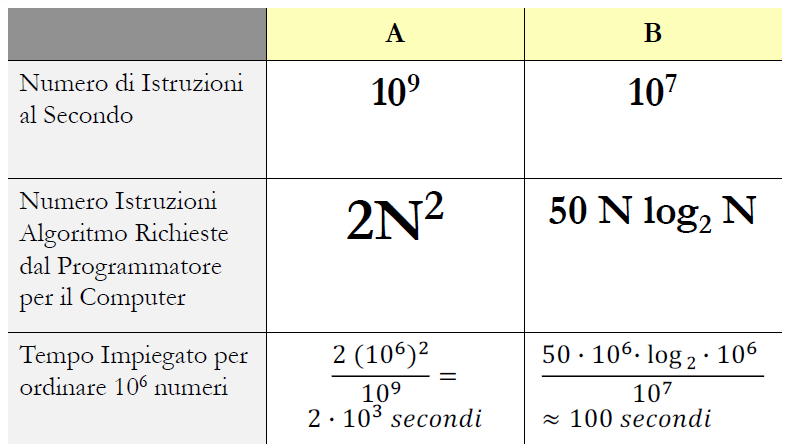
\includegraphics{C:/Users/giova/Documents/1_UNI/programmazione1/appunti/appunti-prog1/image/image-20210105161830403.png}
\caption{image-20210105161830403}
\end{figure}

Inoltre questo ci fa capire che con due algoritmi diversi, se uno è più
efficiente lo è sempre tralasciando l'architettura.

Ci sono classi di algoritmi che sono studiati da anni per essere i
migliori. Ormai infatti esistono algoritmi ottimizzati al massimo per
qualsiasi cosa.

\hypertarget{algoritmi-di-ricerca}{%
\subsubsection{Algoritmi di ricerca}\label{algoritmi-di-ricerca}}

L'algoritmo di ricerca è un algoritmo che permette di trovare un
elemento avente determinate caratteristiche tra un insieme di elementi.
Gli elementi dell'insieme sono caratterizzati da una \emph{chiave} e da
un gruppo di \emph{dati satellite}. Negli algoritmi di ricerca i dati
satellite di solito si ignorano perché non sono utilizzati nella
ricerca. Di conseguenza la chiave dell'elemento acquista una certa
importanza, siccome è quella cosa che deve eguagliare l'elemento
ricercato. Inoltre la chiave può essere \emph{univoca} o
\emph{multipla}, cioè se esiste una sola o più volte nel gruppo di
elementi. Di conseguenza nella ricerca bisogna tener conto se si sta
cercando un singolo elemento, l'ultimo, uno in particolare o se invece
deve restituire tutti i risultati. Per questo bisogna stare attenti ad
usare l'algoritmo corretto adeguato al comportamento che ci si aspetta.

\hypertarget{analisi-complessituxe0-della-ricerca-sequenziale}{%
\paragraph{\texorpdfstring{Analisi Complessità della \emph{ricerca
sequenziale}}{Analisi Complessità della ricerca sequenziale}}\label{analisi-complessituxe0-della-ricerca-sequenziale}}

Dato un determinato insieme di input e un algoritmo, può accadere che
due machine astratte diano luogo a tempi di esecuzione diversi. Di
conseguenza si parla di complessità dell'input e se ne distinguono 3
casi:

\begin{enumerate}
\def\labelenumi{\arabic{enumi}.}
\tightlist
\item
  Caso medio
\item
  Caso peggiore
\item
  Caso migliore
\end{enumerate}

\begin{figure}
\centering
\includegraphics{C:/Users/giova/Documents/1_UNI/programmazione1/appunti/appunti-prog1/image/image-20210105163232538.png}
\caption{image-20210105163232538}
\end{figure}

Nella ricerca sequenziale accade che:

\begin{enumerate}
\def\labelenumi{\arabic{enumi}.}
\tightlist
\item
  Nel \emph{caso peggiore} l'elemento cercato è l'ultimo rispetto
  all'elemento di partenza, quindi il numero di passi necessari a
  raggiungerlo è uguale al numero degli elementi.
\item
  Nel \emph{caso migliore} l'elemento cercato è il primo rispetto
  all'elemento di partenza, quindi il numero di passi necessari al suo
  raggiungimento è 1.
\item
  Nel \emph{caso medio} compaiono tutti gli altri casi, che possono
  essere semplificati con la metà dei valori di input.
\end{enumerate}

E questa descrizione vale solo se io sto cercando la \emph{prima
occorrenza}, infatti se devo trovare tutte le volte che compare un certo
valore la complessità sarà sempre uguale al numero di elementi, perché
non avrò mai la garanzia che tra quelli non controllati non ci sia
un'altra occorrenza. In questo caso quindi la \emph{complessità} media,
migliore o peggiore è \emph{N}.

Un implementazione di questo algoritmo potrebbe essere:

\begin{lstlisting}[language={C++}]
int SequentialSearch(char* item, int cout, char key){
    register int t;
    for (t=0; t<count; ++t){
        // questo algoritmo esce alla PRIMA occorrenza dell'elemento cercato
        if (key == item[t]) return t;
    }
    return -1; // nessuna occorrenza!
}

/*       --- 
 * VARIANTE CON SENTINELLA (se arrivo alla sentinella arrivo sono alla fine)
 *       --- 
 * faccio un array con N elementi in cui cercare e (N+1) = elemento cercato, facendo così posso fare la ricerca con un solo elemento.
 */
int SequentialSearchGuard(char* item, int count, char key){
    
    register int t;
    // Aggiorno il valore sentinella
    item[count] = key;
    // con una sola condizione verifico se sono alla fine o se ho trovato l'elemento
    // fa avanzare t finchè è uguale alla cella o se è vuoto
    for (t = 0; key != item[t]; ++t){
        if (t<count) return t; // found
            else return -1;   // not found
    }
}
\end{lstlisting}

E va notato che è indifferente in questi archivi decidere se scorrere da
destra a sinistra o da sinistra a destra. La keyword
\passthrough{\lstinline!register!} indica di salvare il valore nella
memoria più veloce possibile.

Inoltre l'implementazione con la sentinella permette di ridurre le
condizioni che vengono controllate all'interno del ciclo, ottimizzando
il numero di confronti. La complessità dell'algoritmo però non cambia
anche se abbiamo ridotto le condizioni da valutare.

\hypertarget{analisi-complessituxe0-della-ricerca-sequenziale-in-una-sequenza-ordinata}{%
\paragraph{\texorpdfstring{Analisi Complessità della \emph{ricerca
sequenziale in una sequenza
ordinata}}{Analisi Complessità della ricerca sequenziale in una sequenza ordinata}}\label{analisi-complessituxe0-della-ricerca-sequenziale-in-una-sequenza-ordinata}}

Nella ricerca sequenziale di prima non avevamo dei punti di riferimento
rispetto allo stato dell'input, quindi non sapevamo caratterizzarlo e
neanche in che luogo poterlo andare a prenderlo.

Se invece usassimo un archivio ordinato rispetto a un elemento ad
esempio dal più grande al più piccolo, avremmo potuto sapere qualcosa
dello stato dell'input e quindi avere un punto di partenza per dove
iniziare a cercare.

Per questo motivo un altro algoritmo è quindi la \emph{ricerca in una
sequenza ordinata}. Gli algoritmi che ricercano in un insieme di dati
ordinati sono avvantaggiati perché permettono innanzitutto di fermare la
ricerca nel caso in cui il valore cercato è fuori dal range e in secondo
luogo permettono di trovare subito se ci sono ricorrenze.

Ad esempio in un insieme di numeri, se dovessi trovare il valore 7 e
avessi già passato il valore 8 saprei che mi posso fermare. E allo
stesso modo, se sto cercando una ricorrenza del valore 6, ma dopo il
singolo elemento con questo valore ne trovo uno maggiore a lui, allora
so che il valore 6 compare solo una volta nell'insieme.

Un implementazione tipo di questo algoritmo può essere

\begin{lstlisting}[language={C++}]
int SequentialSearchSorted(char* item, int count, char key){
    
    register int t;
    t=0;
    while( (t<count) && (key>= item[t])){
        if (key == item[t]) return t;
        t++;
    }
    return -1;
    
}
\end{lstlisting}

Questo algoritmo permette quindi di eliminare il dovere di scorrere
sempre tutto l'insieme dei valori nel caso in cui voglio trovare tutte
le ricorrenze, ma non permette però di diminuire la complessità.
Infatti, se il cercassi un valore che è l'ultimo rispetto al mio valore
di partenza io dovrei sempre scorrere tutto l'insieme (descrizione del
caso peggiore).

\hypertarget{algoritmo-di-ricerca-binaria}{%
\subsubsection{Algoritmo di ricerca
binaria:}\label{algoritmo-di-ricerca-binaria}}

La ricerca binaria, che si può chiamare anche dicotomica, necessita di
un accesso casuale ai dati ordinati, di conseguenza non vanno bene
strutture astratte come la lista. Con questi requisiti si può cercare
l'elemento centrale di un insieme ordinato e in base al valore di questo
elemento si cerca avanti o dietro questo elemento. Usando questa tecnica
si dimezza l'insieme in cui si sta cercando ad ogni operazione.

\includegraphics{C:/Users/giova/Documents/1_UNI/programmazione1/appunti/appunti-prog1/image/image-20201206183123802-1609859221338.png}

L'implementazione tipica di questo algoritmo è:

\begin{lstlisting}[language={C++}]
mid = (TOP + BOTTOM)/2;

// confronto su questo elemento:
if (mid == ElCercato) return OK;
if (mid < ElCercato){
    // si sposta la ricerca nella metà superiore dell'insieme
    BOTTOM = (mid+1);
    TOP = TOP;
    mid = (TOP + BOTTOM)/2;
    if (mid < mid){
        ... // si continua in questo modo all'infinito (sotto scritta meglio questa funzione)
    }
}
// logicamente esiste anche il caso mid>ElCercato 
if (mid > ElCercato){
    ...;
    TOP = (mid-1);
    ...; // tutto uguale il resto
} // che esegue esattamente le stesse cose, prendendo però solo il sottoinsieme superiore.
/* cosa succede se non esiste l'elemento
 * Arrivo a un caso in cui BOTTOM > TOP, in questo caso posso fermarmi perchè viene meno la definizione di BOTTOM e di TOP

// La chiave di questa ricerca quindi sono gli indici e l'ordinamento dell'insieme.
\end{lstlisting}

Un implementazione tipo dell'algoritmo di ricerca binaria:

\begin{lstlisting}[language={C++}]
int BinarySearch(char* item, int count, char key){
    int bottom, top, mid;
    bottom = 0;
    top = count -1;
    // creo un ciclo finché BOTTOM e TOP non si invertono
    while (bottom <= top){
        mid = (bottom+top)/2; // Mid è sempre l'elemento centrale per ogni ciclo
        if (key<item[mid]) top = mid-1; // se la cosa cercata è minore dell'elemento in mezzo, allora si prende il sottoinsieme sotto
            else if(key>item[mid]) bottom = mid+1;
        // se la cosa cercata è maggiore del MID, allora si prende il sottoinsieme superiore
        else return mid; // FOUND
    }
    return -1; // Non trovato
}
\end{lstlisting}

Bisogna notare che:

\begin{itemize}
\tightlist
\item
  le keyword \passthrough{\lstinline!TOP!},
  \passthrough{\lstinline!BOTTOM!} e \passthrough{\lstinline!mid!}
  servono ad indicare rispettivamente l'elemento finale, iniziale e
  centrale dell'insieme.
\item
  la funzione è facilmente implementabile anche in modo recursivo
\end{itemize}

Qual è la complessità della ricerca binaria/dicotomica: \[
O(log_2(n))
\] Nel caso peggiore dobbiamo fare questo numero di operazioni per
trovare l'elemento.

Questa inoltre è la prova che il logaritmo di ricerca dicotomica va
meglio della ricerca sequenziale.

Si ricorda che la crescita logaritmica permette di avere un tempo di
esecuzione che cresce molto lentamente rispetto al numero di dati
inseriti rispetto ad altri algoritmi.

\includegraphics{C:/Users/giova/Documents/1_UNI/programmazione1/appunti/appunti-prog1/image/image-20201206185058752-1609859221338.png}

\hypertarget{analisi-dei-tempi-di-esecuzione}{%
\subsubsection{Analisi dei Tempi di
Esecuzione:}\label{analisi-dei-tempi-di-esecuzione}}

\[
Tempo di Esecuzione = T(N)
\]

Dove si prende N la dimensione dei dati di ingresso, e assumiamo che si
prenda il numero di istruzioni come dipendenza per il tempo di
esecuzione. (Ovvero non consideriamo aspetti dinamici dell'esecuzione
dell'algoritmo).

Queste funzioni, che appunto indicano il tempo di esecuzione, possono
avere molti elementi che le compongono, che possono contare di più o di
meno.

Es: \[
T(N) = 1 + N + N^2 + log(N)
\] In cui:

\begin{itemize}
\tightlist
\item
  1 = Elemento costante
\item
  N = Componente lineare
\item
  N\^{}2 = parte quadratica, nonché quella che cresce più velocemente
\end{itemize}

Spesso però non servono queste funzioni dirette, ma alcune funzioni che
permettano di delimitare la crescita di una funzione. Per questo ci
viene in aiuto la notazione \emph{O} (anche chiamata \emph{BigO}).

Questa notazione fornisce il limite superiore ad una funzione, anche
delimitatamente in un intervallo. \[
f(n) = O(g(n))
\]

Mentre un'altra funzione ci permette di ingabbiare questa funzione dal
basso. \[
f(n) = Ω(g(n))
\] Unendo queste due funzioni, si ottiene una terza funzione che, dato
che riesce a indicare i massimi punti che toccherà con \emph{O}, e i
minimi punti con \emph{Ω}, allora la funzione che ne risulta sarà una
stima della funzione stessa (ovvero f(n) si comporterà più o meno come
g(n)). \[
f(n) = Ɵ(g(n))
\] Tutti questi ragionamenti, logicamente valgono in intervalli
limitati.

\hypertarget{ricapitolando}{%
\paragraph{Ricapitolando}\label{ricapitolando}}

\begin{itemize}
\tightlist
\item
  abbiamo il \textbf{caso peggiore/minore/medio} di T(n) a seconda
  dell'input.
\item
  La notazione \textbf{O/Omega/Theta} che indica invece come la funzione
  si approssima.
\end{itemize}

Esempi:

\begin{itemize}
\item
  la T(n) di un'operazione \emph{push()} su uno stack: \[
  Ɵ(1)
  \] ( Per quando male, andrà sempre uguale).
\item
  Inserimento di un elemento in una coda FIFO in un array circolare: \[
  Ɵ(1)
  \]
\item
  Ricerca sequenziale in un array non ordinato, nel caso peggiore \[
  Ɵ(N)
  \]
\item
  Ricerca sequenziale in un array non ordinato, caso medio: \[
  Ɵ(1)
  \]
\end{itemize}

\hypertarget{algoritmi-di-ordinamento}{%
\subsubsection{Algoritmi di
ordinamento}\label{algoritmi-di-ordinamento}}

L'ordinamento degli array o degli insieme è spesso richiesto affinché
siano efficienti i calcoli su questi insiemi o per l'esecuzione di
alcuni algoritmi che necessitano di un insieme ordinato, come ad esempio
la ricerca dicotomica. Alcuni problemi invece necessitano di questi
algoritmi per essere risolti, come il problema della ricerca della
mediana.

In questa sezione vedremo gli esempi più importanti di algoritmi di
ordinamento con rispettiva analisi della complessità. Questa analisi
sarà fatta sia per il calcolo del \emph{T(n)} e del \emph{O}.

In particolare vedremo l'\textbf{insertion-sort} e il
\textbf{merge-sort}, che rappresentano anche due macroclassi di
complessità per gli algoritmi.

\hypertarget{algoritmo-insertion-sort}{%
\paragraph{\texorpdfstring{Algoritmo
\emph{insertion-sort}:}{Algoritmo insertion-sort:}}\label{algoritmo-insertion-sort}}

Questo algoritmo è efficiente per array di piccole dimensioni, quindi
non è sempre una via da escludere rispetto agli altri. Concettualmente è
come prendere una carta alla volta e posizionarle correttamente in un
altro mazzo, quindi il problema più grande è quello di non creare
disordine nel mazzo, in modo che poi le carte che verranno inserite dopo
siano al posto giusto.

Le operazioni che eseguirò sono:

\begin{itemize}
\tightlist
\item
  estraggo il primo valore (A) e lo posiziono all'inizio
\item
  estraggo il secondo valore: se questo è maggiore lo metto dopo
  l'elemento precedentemente posizionato e se questo è minore lo metto
  prima. Questa operazione si può anche descrivere come un confronto tra
  l'ultimo elemento ordinato e il primo elemento non ordinato.
\end{itemize}

\begin{figure}
\centering
\includegraphics{C:/Users/giova/Documents/1_UNI/programmazione1/appunti/appunti-prog1/image/image-20201207115753626.png}
\caption{image-20201207115753626}
\end{figure}

E la complessità asintotica dell'algoritmo è:

\begin{itemize}
\tightlist
\item
  nel caso \emph{medio}:
\end{itemize}

\[
Theta(N^2)
\]

\begin{itemize}
\tightlist
\item
  nel caso \emph{peggiore} (ovvero quando devo completamente girare
  l'array):
\end{itemize}

\[
Theta(N^2)
\]

Questo impone all'algoritmo di essere efficiente solo con \emph{N}
sufficientemente piccoli.

La complessità prende questo valore perché ho due cicli annidati, come
si vede anche nel codice: uno che scorre l'array di partenza e uno che
scorre l'array di arrivo.

\begin{lstlisting}[language={C++}]
void InsertionSort(A){
    n = DimensioneArray(A);
    for (int j=1; j<n; ++j){
        // Prendo la carta da inserire
        x = A[j];
        // Secondo indice, quello del ciclo annidato. é anche l'indice superiore, che indica il sottoArray tra 0->(j-1).
        i = j-1;
        /* controllo di non essere alla fine dell'array.
         * Quando trovo il caso in cui x < ElementoArray[i], allora
         * assegno la carta a quel posto
         */
        while( (i >= 0) && (x<A[i])){
            A[i+1] = A[i];
            i = i-1;
        }
        // Prendo la prossima carta.
        A[i+1] = x;
    }
}
\end{lstlisting}

\hypertarget{analisi-di-complessituxe0-del-insertion-sort}{%
\subparagraph{\texorpdfstring{Analisi di complessità del
\emph{insertion-sort}:}{Analisi di complessità del insertion-sort:}}\label{analisi-di-complessituxe0-del-insertion-sort}}

Posso eseguire un calcolo sulla complessità dell'algoritmo in modo
statico, attraverso la logica dei cicli e assegnando a ogni linea il
contributo sulla complessità:

\begin{lstlisting}[language={C++}]
void InsertionSort(A){
    n = DimensioneArray(A);
    for (int j=1; j<n; ++j){          // c1*n
        x = A[j];                    // c2*(n-1)
        i = j-1;                     // c3*(n-1)
        while( (i >= 0) && (x<A[i])){ // c4 * (sommatoria da j=2 a n di tj)
            A[i+1] = A[i];           // c5 * (Sommatoria da j=2 a n di (tj-1))
            i = i-1;                // c6 * (Sommatoria da j=2 a n di (tj-1))
        }
        A[i+1] = x;                 // c7 * (n-1)
    }                            // ------------------------
}                               // La somma di queste complessità porta alla funzione T(n), dove n è il numero di operazioni.
\end{lstlisting}

Da questa ne esce un un insieme di equazioni contenente \emph{c} con un
valore numerico che sono costanti, e una serie con \emph{t} che segna il
numero delle operazioni per \emph{j} volte.

Per arrivare a delle equazioni calcolabili, introduciamo, per logica la
complessità nel \emph{caso migliore} che è: \[
t_j = 1
\]

perché il primo confronto è già falso, quindi non eseguo mai il corpo
istruzioni del \passthrough{\lstinline!while!}. Questa situazione si può
anche descrivere dicendo che in questo caso \emph{l'array è ordinato in
partenza}.

Sapendo questo dato posso tradurre le equazioni di complessità come:

\begin{lstlisting}[language={C++}]
void InsertionSort(A){
    n = DimensioneArray(A);
    for (int j=1; j<n; ++j){          // c1*n
        x = A[j];                    // c2*(n-1)
        i = j-1;                     // c3*(n-1)
        while( (i >= 0) && (x<A[i])){ // c4*(n-1)
            A[i+1] = A[i];           // 0
            i = i-1;                // 0
        }
        A[i+1] = x;                 // c7 * (n-1)
    }                            // ------------------------
}                               // quindi posso calcolare e trovare Omega.
\end{lstlisting}

Che quindi è rappresentabile: (Dove \emph{T} rappresenta il numero di
operazioni per \emph{N} elementi) \[
T(n) = (c1+c2+c3+c4+c7) * n = bn + a = Θ(n)
\] Da questo posso dedurre che la complessità del caso migliore è
lineare.

Eseguiamo adesso lo stesso calcolo nel caso sia preso in considerazione
il \emph{caso peggiore}, cioé: \[
t_j = n
\] Questa operazione significa che io devo completamente girare il mio
array di valori, e di conseguenza il numero di operazioni è uguale al
numero dei valori che questo array contiene.

Da questa relazione possiamo quindi tradurre il \emph{caso generale} e
trovare la complessità del caso peggiore:

\begin{lstlisting}[language={C++}]
void InsertionSort(A){
    n = DimensioneArray(A);
    for (int j=1; j<n; ++j){          // c1*n
        x = A[j];                    // c2*(n-1)
        i = j-1;                     // c3*(n-1)
        while( (i >= 0) && (x<A[i])){ // c4*(sommatoria da j=2 fino a n)
            A[i+1] = A[i];           // 0
            i = i-1;                // 0
        }
        A[i+1] = x;                 // c7 * (n-1)
    }                            // ------------------------
}                               // Posso calcolare

\end{lstlisting}

Che si traduce in: \[
T(n) = c_1n+c_2n+c_3(n-1)+c_4\sum_{j=2}^{n} j + c_5\sum_{j=2}^{n}(j-1) + c_6\sum_{j=2}^{n}(j-1) + c_7(n-1)
\] Poi si sa che: \[
\sum_{j=2}^{n} j = {n(n+1) \over 2} -1
\]

\[
\sum_{j=2}^{n} (j-1) = {n(n+1) \over 2} - n = {n(n-1) \over 2}
\]

Possiamo quindi tornare e sostituire i contributi: \[
T(n) = c_1n+c_2(n-1)+c_3(n-1)+c_4({n(n+1) \over 2} - 1) + c_5({n(n-1) \over 2})  + c_4({n(n-1) \over 2})  + c_7(n-1)
\]

\[
T(n) = {1 \over 2}(c_4*c_5+c_6)n^2 + (c_1+c_2+c_3+{1 \over 2}c_4 - {1 \over 2}c_5 - {1 \over 2}c_6 + c_7)n -c_2 -c_3-c_4-c_7 \\\\
= c'n^2+b'n+a' \rightarrow Θ(n^2)
\]

Con queste ultime operazioni siamo quindi riusciti a definire il
comportamento dell'\emph{insertion-sort}, trovando il suo valore
asintotico.

\hypertarget{categorie-di-algoritmi-che-si-comportano-come-linsertion-sort}{%
\subparagraph{\texorpdfstring{Categorie di algoritmi che si comportano
come
l'\emph{insertion-sort}:}{Categorie di algoritmi che si comportano come l'insertion-sort:}}\label{categorie-di-algoritmi-che-si-comportano-come-linsertion-sort}}

Ricapitolando, l'\emph{insertion-sort} è un algoritmo che:

\begin{itemize}
\tightlist
\item
  fa l'ordinamento \emph{sul posto}, usa quindi un solo array senza
  necessità di array d'appoggio.
\item
  confronta e scambia tra loro elementi consecutivi dell'array.
\end{itemize}

Da queste informazioni possiamo dedurre che:

\textbf{Teorema:} La \emph{complessità nel caso peggiore} per ogni
algoritmo di ordinamento che si comporta come l'\textbf{insertion-sort}
è al massimo: \[
Θ(n^2)
\]

Algoritmi più efficienti richiedono scambi tra elementi distanti
dall'array.

\hypertarget{algoritmo-di-merge-sort}{%
\paragraph{\texorpdfstring{Algoritmo di
\emph{merge-sort}:}{Algoritmo di merge-sort:}}\label{algoritmo-di-merge-sort}}

L'algoritmo di \emph{merge-sort} si comporta nel caso peggiore: \[
Θ(n * log(n))
\] e ha la particolarità di unire due concetti:

\begin{enumerate}
\def\labelenumi{\arabic{enumi}.}
\tightlist
\item
  la ricorsione
\item
  Divide et Impera (operazione di fusione per unire i sotto-array)
\end{enumerate}

Come funziona:

\begin{itemize}
\tightlist
\item
  si prende l'array e si divide in due metà, si creano quindi due
  sotto-problemi
\item
  continuo a dividere ancora in due sotto-array finché non arrivo alla
  soluzione base, ovvero un sotto-array di dimensione 1.
\item
  Arrivato all'array di 1 elemento, allora restituisco l'array ordinato.
\item
  Da questi due array diversi unisco (\emph{merge}) e genero un array
  che è la somma nell'ordine corretto degli array in ingresso.
\end{itemize}

\begin{lstlisting}[language={C++}]
// Array = A, indice destro = p, indice sx = r
MergeSort(A, p, r){
    if(p<r){
        // trovo il punto centrale -> DIVIDE
        q = Floor((p+r)/2);
        // Sottoinsieme sx -> Chiamata ricorsiva (IMPERA)
        MergeSort(A, p, q);
        // Sottoinsieme dx -> Chiamata ricorsiva (IMPERA)
        MergeSort(A, q+1, r);
        // Unisce i due sottoinsieme -> Funzione principale
        Merge(A, p, q, r);
    }
    // caso base
}

// Vettore A, indici p, w, r = dx, centrale, sx
Merge(A, p, q r){
    // Sottoarray sinistro
    n1 = q-p+1;
    // Sottoarray destro
    n2 = r-q;
    // tutti questi elementi tra p-q-r sono ordinati!
    int j, i;
    // Riempio gli array
    for (i=0; i<n1; ++i){ L[i] = A[p+i]; }
    for (j=0; j<n2; ++j){ R[j] = A[q+1]; }
    // Valore sentinella
    L[n1] = R[n2] = MAXINT;
   // aggiorno intanto che faccio i confronti
    i=j=0;
    // r - p+1 passi
    for(int k=p, k<=r; ++k){ 
        if ( L[i] <= R[j] ){
            A[k] = L[i];
            i++;
        } else{
            A[k] = R[j];
            j++;
        }
    }
}
\end{lstlisting}

\#\#\#\#\# Analisi dei tempi di esecuzione del \emph{merge-sort}:

Principalmente si prende in considerazione il tempo della funzione
\passthrough{\lstinline!Merge()!}: \[
T_{merge}(n) = Θ(n) \\
Θ(n) = Θ(r-p+1)
\] Quindi nel caso peggiore, l'algoritmo di \emph{merge-sort} ha
complessità \[
Θ(n log(n))
\] Questo valore arriva per il calcolo delle complessità in funzioni
ricorrenti, dove si mette a sistema il caso base e il caso ricorsivo: \[
T(n) =
\bigg \{
\begin{array}{}
Θ(1) \text{ Se } n \leq c \\
aT({n \over b}) + D(n) + C(n)  \\
\end{array}\\
\] Dove:

\begin{itemize}
\tightlist
\item
  \passthrough{\lstinline!c!}: costante piccola
\item
  \passthrough{\lstinline!a!} : numero sotto-problemi generato dal passo
  \emph{divide}
\item
  \passthrough{\lstinline!1/b!} : dimensione dei sotto-problemi rispetto
  a quello a quello originale
\item
  \passthrough{\lstinline!D(n)!} : Tempo/Risorse impiegato per dividere
  i problemi in sotto-problemi (operazione di
  \passthrough{\lstinline!Floor!})
\item
  \passthrough{\lstinline!C(n)!} : Tempo impiegato per ricombinare le
  sotto-soluzioni
\end{itemize}

Nel caso di \emph{merge-sort} l'equazione di ricorrenza ha i seguenti
parametri: \[
a = 2 \\
b=2\\
T_{MergeSort}(n) = 
\bigg \{
\begin{array}{}
Θ(1) \text{ Se } n \leq c \\
2T({n \over 2}) + D(n) + C(n)  \\
\end{array}\\
\] Il termine \emph{divide} ovvero \passthrough{\lstinline!D(n)!},
corrisponde al calcolo della metà (cioè quello che restituisce
\passthrough{\lstinline!Floor!}) \[
D(n) = Θ(1) \text { (è un valore costante)}\\
\text{Impera: } = 2T({n \over 2}) \\
C(n) : \text {Operazione combinazione/fusione} \\
C(n) = Θ(n)
\] E a questo punto siccome \passthrough{\lstinline!a=b=2!} e ricordando
che dall'operazione sopra ci risulta questo: \[
Θ(n) \leftarrow C(n) = Θ(n) \\
Θ(n) \leftarrow D(n) = Θ(1)
\]

possiamo scrivere che: \[
T_{MergeSort}(n) = 
\bigg \{
\begin{array}{}
Θ(1) \text{ Se } n \leq c \\
2T({n \over 2}) + Θ(n) \\
\end{array}\\
\]

Ma nel caso dell'\emph{insertion-sort} ottengo un polinomio, quindi non
riesco a trovare la complessità statica totale.

Le equazioni di ricorrenza si possono essere risolte in vari modi ad
esempio la sostituzione o l'albero di ricorsione.

\hypertarget{risoluzione-della-complessituxe0-della-ricorsione-con-il-metodo-dellalbero-di-ricorsione}{%
\subparagraph{\texorpdfstring{Risoluzione della complessità della
ricorsione con il \emph{metodo dell'albero di
ricorsione}}{Risoluzione della complessità della ricorsione con il metodo dell'albero di ricorsione}}\label{risoluzione-della-complessituxe0-della-ricorsione-con-il-metodo-dellalbero-di-ricorsione}}

Dal sistema di prima possiamo fare alcune deduzioni:

\begin{itemize}
\tightlist
\item
  il significato di \emph{Θ(1)} è che si approssima a una funzione
  lineare, che vuol dire una funzione costante
\item
  quindi si può sostituire \emph{Θ(1)} con \emph{C} e \emph{Θ(n)} con
  \emph{Cn}
\end{itemize}

Da queste deduzioni otteniamo dei termini espliciti: \[
T_{MergeSort}(n) = 
\bigg \{
\begin{array}{}
C \text{ Se } n = 1 \\
2T({n \over 2}) + Cn \text{ Se n>1} \\
\end{array}\\
\]

Che si può risolvere attraverso la creazione di un \emph{albero di
ricorsione}:

\begin{figure}
\centering
\includegraphics{C:/Users/giova/Documents/1_UNI/programmazione1/appunti/appunti-prog1/image/Untitled Diagram.jpg}
\caption{Untitled Diagram}
\end{figure}

E si continua in questo modo finché non si è trovato il caso di base,
che costa \emph{c}, di conseguenza l'ultimo ``piano'' di rami
dell'albero sono \emph{n} foglie che costano ognuna \emph{C}. (quindi
\emph{n*C})

Poi dovremmo calcolare il numero di livelli che impiego ad arrivare al
caso base e il rispettivo costo.

Dovremmo risolvere 3 problemi quindi:

\begin{enumerate}
\def\labelenumi{\arabic{enumi}.}
\tightlist
\item
  Calcolare il numero di livelli
\item
  Calcolare il numero delle foglie
\item
  calcolare il costo di \emph{Ci} (costi di ciascun livello)
\end{enumerate}

Se risolviamo 1, 2, 3 troviamo \emph{T(n)} sommando i costi di tutti i
livelli, inclusi i costi delle foglie.

Il costo di ciascun livello si può scrivere anche in questo modo: \[
C_1 \rightarrow Cn \\
C_2 \rightarrow C(n/2) + C(n/2) = Cn \\
C_3 \rightarrow C(n/4) + C(n/4) + C(n/4) + C(n/4) = C(n) \\
\] Che in generale: \[
C_i = 2^i * c\big({n \over 2^i}\big) = cn \\
C_{NumLivel.} := cn
\] Quindi il costo di ciascun livello del \emph{merge-sort} è \emph{Cn}.
Di conseguenza: \[
T(n) = \sum_{i}^{NumLivel} C_i
\] Il calcolo dei numero dei livelli viene fatto per \emph{induzione}:
(si conosce la soluzione per un caso base e si risolve per un caso
generico). Cioè:

IPOTESI: \[
NumLivelli = log_2(n+1)
\] da questo, il CASO BASE: \[
n = 1 \\
NumLivelli = 1 = 0+1 \rightarrow OK!
\] CASO INDUTTIVO: \[
n = 2^i \\
NumLivelli = log(2^i+1) = i+1
\] Noi sappiamo che ogni volta che passiamo di livello, moltiplichiamo
per due nel livello successivo, quindi: \[
ProssimoN : n=2^{i+2} \\
n = 2^{i+1} \\
(i+1) +1 = log_2(2^{i+1}) + 1
\] Che quindi dimostra la formula per il caso bersaglio che stavamo
cercando.

Con questo possiamo descrivere il caso induttivo. Da questo ragionamento
arriviamo nell'ultimo caso, nel quale dobbiamo sommare tutti le somme
parziali dei livelli: \[
\sum_i^{NulLivelli}C_i \\
T(n) = cn * NumLivelli = cn * (logn +1) \\
 = cnlog(n) + cn = - (nlog(n))
\] E con questa si dimostra come il \emph{merge-sort} ha complessità
costante, sia nel caso peggiore che nel caso migliore e vale: \[
Θ(nlog(n))
\]

\hypertarget{risoluzione-della-complessituxe0-della-ricorsione-con-il-metodo-della-sostituzione}{%
\subparagraph{\texorpdfstring{Risoluzione della complessità della
ricorsione con il \emph{metodo della
sostituzione}}{Risoluzione della complessità della ricorsione con il metodo della sostituzione}}\label{risoluzione-della-complessituxe0-della-ricorsione-con-il-metodo-della-sostituzione}}

Come prima partiamo dalla complessità della funzione che è: \[
T_{MergeSort}(n) = 
\bigg \{
\begin{array}{}
Θ(1) \text{ Se } n \leq c \\
2T({n \over 2}) + Θ(n) \\
\end{array}\\
\]

Voglio dimostrare che \emph{T(n) = Θ(nlog(n))}.

Dimostrare per induzione che: \[
T(n) = cn*log(n) \text{ per } c < 0 
\] Assumo che il CASO BASE: \[
T(1) = Θ(1)
\] e il CASO INDUTTIVO:

Assumo che la diseguaglianza valga per n\textless k. Che quindi \[
T(n) \leq cn*log(n)
\] Dimostrare che questa sopra vale per n=k, in particolare n=K/2. \[
T({k \over 2}) \leq c{k \over 2}log({k \over 2})
\] La ricorsione ci dice che: \[
T(k) = 2T({k \over 2}) + k \\
T(k) \leq 2c({k \over 2})log({k \over 2}) + k \\
T(k) \leq ck(log(k)-log(2)) + k \\
T(k) \leq cklog(k) - ck + k \\
T(k) \leq cklog(k) + k(1-c) \\
T(k) \leq cKlog(k) +(1-c)k \\
T(k) \leq cklog(k) \\
\text{ per } c \geq 1
\] Questo vuol dire che l'assunto vale per \emph{k\textgreater n},
rispetto all'ipotesi che era più ristretta.

\hypertarget{ricapitolando-algoritmi-di-ordinamento}{%
\paragraph{\texorpdfstring{Ricapitolando \emph{algoritmi di
ordinamento}}{Ricapitolando algoritmi di ordinamento}}\label{ricapitolando-algoritmi-di-ordinamento}}

Gli algoritmi di ordinamento sono dipendenti:

\begin{enumerate}
\def\labelenumi{\arabic{enumi}.}
\tightlist
\item
  dal tipo di elementi da ordinare
\item
  dal verso di ordinamento: crescente o decrescente
\end{enumerate}

Inoltre il \emph{teorema dell'insertion-sort} afferma che i metodi
basati su confronti e scambi sul posto che ordinano una sequenza di
\emph{N} numeri non può fare meglio che \emph{Θ(N\^{}2)} {[}Esempio:
InsertionSort, BubbleSort{]}.

Mentre con gli algoritmi basati sui confronti si può arrivare nel caso
\emph{peggiore} a complessità \emph{Θ(nlog(n))}. {[}Esempio MergeSort,
QuickSort{]}.

Inoltre si può anche dimostrare che \textbf{tutti i metodi per confronto
hanno metodo ottimale al massimo come \emph{nlog(n)}}.

Per migliorare ancora la complessità di algoritmi di ordinamento quindi
bisogna abbandonare il metodo dei confronti e si può arrivare a
complessità inferiore a \emph{nlog(n)}. {[}Esempio CountingSort,
RadixSort, BucketSort{]}.

\end{document}
